\documentclass[11pt]{article}
\usepackage{debulletin,times,epsfig,subfigure,wrapfig,algorithmic,color,boxedminipage,graphicx,url}
% this is the template for an issue of the Data Engineering Bulletin

% all packages used by any paper must be listed here
%\usepackage{hyperref}
%\usepackage{authblk}
%\setlength{\affilsep}{0em}
%\usepackage{inputenc}
%\usepackage{debulletin}
%\usepackage{times}
%\usepackage{graphicx}
%\usepackage{array}
%\usepackage{wrapfig}
%\usepackage[table]{xcolor}
%\usepackage{tcolorbox}
%\usepackage{amssymb}
%%\usepackage[labelfont=bf,labelsep=space,list=true]{subcaption}
%\usepackage{url}
%\usepackage{mathtools, bm}
%\usepackage{float}
%\usepackage{multirow}
%\usepackage{multicol}
%\usepackage{algorithm}
%\usepackage{subfig}
%\usepackage{algpseudocode}
%\setlength{\intextsep}{10pt plus 2pt minus 2pt}
%\hyphenation{finally}

\usepackage{amsmath, amssymb, amsfonts}

\usepackage{hyperref}
\usepackage{enumitem}
\usepackage{xspace} 
%\usepackage{xcolor}
\usepackage{tikz}
\usepackage[T1]{fontenc}
\usepackage{beramono}
\usepackage{listings}
\usepackage{xcolor}

\usepackage{wrapfig}

\usepackage{graphics}
\usepackage{pifont}
\usepackage{makecell}


%\usepackage{subcaption} % for subtable
%\usepackage{threeparttable} % for tablenotes




\usepackage[numbers]{natbib}
% \documentclass{article}
% Recommended, but optional, packages for figures and better typesetting:
\usepackage{microtype}
\usepackage{graphicx}
% \usepackage{subfigure}
\usepackage{booktabs} % for professional tables
%\usepackage[table,dvipsnames]{xcolor}
\usepackage{epsfig}
\usepackage{pgfplotstable}
\usepackage{pgfplots}
\usepgfplotslibrary{groupplots}
\usepackage{bbm}
\usepackage{booktabs}
\usepackage{verbatim}
\usepackage[T1]{fontenc}
\usepackage{caption}
\usepackage{siunitx}
\usepackage{xspace}
%\usepackage[colorinlistoftodos,textsize=footnotesize]{todonotes}
%\usepackage[utf8]{inputenc}

\usepackage[autostyle, english=american]{csquotes}

\usepackage{breakurl}
\usepackage{tabularx}
\usepackage[super]{nth}   
\usepackage{multicol}
\usepackage[]{algorithm2e}

\begin{document}


% please enter real date, vol no, issue no
\bulletindate{December 2021}
\bulletinvolume{44}
\bulletinnumber{4}
\bulletinyear{2021}

% these are files that I have- but your part of the issue can be done without
% them
\IEEElogo{cs.pdf}
\insidefrontcover{incvA19.pdf}
%\insidebackcover[ICDE Conference]{./calls/icde-new-a.ps}

\begin{bulletin}

% the above samples assume the issue is generated from a directory structure of the following sort
% major directory name is month and year of issue
% there are sub-directorys for
% letters: directory name is "letters"
% technical articles: a directory per paper, named for an "author"
% news articles: directory name is "news"
% calls: directory name is "calls

%
%  Editor letters section.  Use the lettersection environment.
%  Each letter is contained in a letter environment, where the two required
%  options to \begin{letter} are the author and the address of the author.
%

\begin{lettersection}

% there will be other letters- and a blank page will appear in your document
% but the special issue part will be fine

\begin{letter}{Letter from the Editor-in-Chief}
{Haixun Wang}{Instacart}
\documentclass[11pt]{article} 

\usepackage{deauthor,times,graphicx}
%\usepackage{url}
\usepackage{hyperref}

\begin{document}
Around the time we published our last issue in March, the nation went
into a lockdown. Life in the last 3 months has been unprecedented in
many ways. As governments around the world scrambled to fight
coronavirus, people in the scientific community, especially those on
the frontline -- doctors, healthcare professionals, medical staff and
researchers -- made heroic efforts and sacrifices to curb the pandemic
and save lives. The data management and data science communities also
sprang to action immediately. Globally, it is the first time that data
driven approaches are being used at such a large scale toward solving
a common problem. Under this backdrop, in this special issue of the
Data Engineering Bulletin edited by Joseph Gonzalez, we feature 8
papers on the topic of {\it digital contact tracing}, a technique that
may prove crucial in the fight against Covid-19.

This issue also features two opinion pieces. Divyakant Agrawal and Amr
El Abbadi's wake-up call on managing data in an untrusted environment
takes us to the fascinating world of cryptocurrencies and
blockchains. It shows what the database community, which was
responsible for creating and perfecting transaction management and
distributed systems, can learn from the blockchain approach when it
comes to handling untrusted behaviours from the underlying
infrastructure. The second opinion piece, written by Jeffrey
D. Ullman, addresses a question on the mind of every data management
person: What is our role in the machine learning and AI revolution?
Have we missed the boat again and become irrelevant? Ullman's
perspective, illustrated by his remake of the well known Conway Venn
Diagram that illustrates the relationship between computer science,
mathematics \& statistics, and domain knowledge is incisive,
thought-provoking, and entertaining at the same time.
\end{document}


\end{letter}
%
\newpage
%
%% your introductory letter goes here
%
%\begin{letter}{Letter from the Special Issue Editor}
\begin{letter}{Letter from the Special Issue Editors} %JF: made it editors, plural
{Shimei Pan and James Foulds}{University of Maryland, Baltimore County}
\documentclass[11pt]{article} 

\usepackage{deauthor,times,graphicx}
%\usepackage{url}

\begin{document}

Software applications that learn from data using machine learning (ML) are being deployed in increasing numbers in the real world. Designing and operating such applications introduces novel challenges, which are very different from the challenges encountered in traditional data processing scenarios. ML applications in the real world exhibit a much higher complexity than ``text book'' ML scenarios (e.g., training a classifier on a pre-existing dataset). They do not only have to learn a model, but must define and execute a whole ML pipeline, which includes data preprocessing operations such as data cleaning, standardisation and feature extraction in addition to learning the model, as well as methods for hyperparameter selection and model evaluation. Such ML pipelines are typically deployed in systems for end-to-end machine learning, which require the integration and validation of raw input data from various input sources, as well as infrastructure for deploying and serving the trained models. The system must also manage the lifecycle of data and models in such scenarios, as new (and potentially changing) input data has to be continuously processed, and the corresponding ML models have to be retrained and managed accordingly. The majority of these challenges have only recently begun to attract the attention of the data management community. 
%
A major obstacle is that the behavior of ML-based systems heavily depends on the consumed input data, which can rapidly change, for example due to changed user behavior or due to errors in external sources that produce the inputs. This area represents a gap between the data management and ML communities: research in ML mostly focuses on learning algorithms, and research in data management is mostly concerned with data processing and integration. In this issue, we focus on this gap in data validation for machine learning, and provide perspectives from both the academic and industrial research communities to learn about the state of the art, open problems and to uncover interesting research directions for the future.

The first paper presents \textit{A Data Quality-Driven View of MLOps} and demonstrates how different aspects of data quality propagate through various stages of machine learning development. It connects data quality to the downstream machine learning process, an approach that is also taken by our second paper, which argues that we should move \textit{From Cleaning before ML to Cleaning for ML}. The authors propose an end-to-end approach to take the entire application's semantics and user goals into account when cleaning data, instead of performing the cleaning operations in an isolated manner beforehand.

The next two papers on \textit{Validating Data and Models in Continuous ML pipelines} and \textit{Automated Data Validation in Machine Learning Systems} from Google and Amazon provide us with an industry perspective on the area in the focus of this issue. The first paper describes tools developed at Google for the analysis and validation of two of the most important types of artifacts: Datasets and Models. These tools (which are part of the Tensorflow Extended Platform) are currently deployed in production at Google and other large organizations, and are heavily inspired by well-known principles of data-management systems. The second paper from Amazon reviews some of the solutions developed to validate data at the various stages of a data pipeline in modern ML applications, discusses to what extent these solutions are being used in practice, and outlines research directions for the automation of data validation.

The subsequent paper on \textit{Enhancing the Interactivity of Dataframe Queries by Leveraging Think Time} focuses on the highly exploratory and iterative nature of data validation in the early stages of an ML application, where data scientists start with a limited understanding of the data content and quality, and perform data validation through incremental trial-and-error. The final paper of this issue on \textit{Responsible AI Challenges in End-to-end Machine Learning} completes the view on data validation for machine learning by connecting it with pressing issues from the area of responsible data management.\\ 

Working on this issue has been a privilege for me, and I would like to thank the authors for their  contributions.


\end{document}


\end{letter}

\end{lettersection}

% put the name of your special issue below

%\begin{opinionsection}
%\begin{opinion}{Entities with Quantities}
%{Gerhard Weikum}{Max Planck Institute for Informatics}
%\documentclass[11pt]{article} 

\usepackage{deauthor,times,graphicx}
%\usepackage{url}
\usepackage{hyperref}

\begin{document}
Around the time we published our last issue in March, the nation went
into a lockdown. Life in the last 3 months has been unprecedented in
many ways. As governments around the world scrambled to fight
coronavirus, people in the scientific community, especially those on
the frontline -- doctors, healthcare professionals, medical staff and
researchers -- made heroic efforts and sacrifices to curb the pandemic
and save lives. The data management and data science communities also
sprang to action immediately. Globally, it is the first time that data
driven approaches are being used at such a large scale toward solving
a common problem. Under this backdrop, in this special issue of the
Data Engineering Bulletin edited by Joseph Gonzalez, we feature 8
papers on the topic of {\it digital contact tracing}, a technique that
may prove crucial in the fight against Covid-19.

This issue also features two opinion pieces. Divyakant Agrawal and Amr
El Abbadi's wake-up call on managing data in an untrusted environment
takes us to the fascinating world of cryptocurrencies and
blockchains. It shows what the database community, which was
responsible for creating and perfecting transaction management and
distributed systems, can learn from the blockchain approach when it
comes to handling untrusted behaviours from the underlying
infrastructure. The second opinion piece, written by Jeffrey
D. Ullman, addresses a question on the mind of every data management
person: What is our role in the machine learning and AI revolution?
Have we missed the boat again and become irrelevant? Ullman's
perspective, illustrated by his remake of the well known Conway Venn
Diagram that illustrates the relationship between computer science,
mathematics \& statistics, and domain knowledge is incisive,
thought-provoking, and entertaining at the same time.
\end{document}


%\end{opinion}
%\end{opinionsection}

\begin{articlesection}{Responsible AI and Human-AI Interaction}
%
%  Contributed articles section.  Use the articlesection environment.
%  Each article is contained in an article environment, where the two required
%  options to \begin{article} are the title and author of the article
%

%\makeatletter
%\renewcommand{\AB@affillist}{}
%\renewcommand{\AB@authlist}{}
%\setcounter{authors}{0}
%\makeatother

\begin{article}
{AI-Enhanced Adaptive Assistive Technologies: Methods for AI Design Justice}
{Nora McDonald, Aaron, Massey, and Foad Hamidi}
\graphicspath{{submissions/McDonald_final/}}
\documentclass[11pt,dvipdfm]{article}
%\documentclass[11pt]{article} The above line must be used for your camera-ready submission, which requires a latex -> DVI -> PDF compilation pipeline.  As a workaround while you are writing your paper, you could comment it out and use this line instead, which is compatible with pdflatex.%
\usepackage{deauthor,times,graphicx,hyperref} 

\begin{document}
\title{AI-Enhanced Adaptive Assistive Technologies: Methods for AI Design Justice}
\author{Nora McDonald*, Aaron, Massey**, and Foad Hamidi**\\ 
University of Cincinnati* and University of Maryland, Baltimore County**\\ 
mcdonnan@ucmail.uc.edu, akmassey@umbc.edu, foadhamidi@umbc.edu}


\maketitle
\begin{abstract}
The design of artificial intelligent (AI) enhanced adaptive assistive technologies (AATs) presents exciting promise for those with motor or audio/vision impairment. However, these technologies also introduce tremendous privacy risks, particularly for those with compounding identity vulnerabilities. In this paper, we reflect on why and how AATs need to be designed in collaboration with intersectional AAT users to ensure that the benefits of AI do not sacrifice privacy for the most vulnerable. We discuss methods and tools we have developed to meet these challenges, lessons we have learned from studies with them, and future opportunities.
\end{abstract}

\section{Introduction}
AI systems can compound discriminations of those with disabilities. Based on individual’s social media profiles, smartphones settings, or performance data, one can infer whether individuals are blind \cite{40} or have symptoms of Parkinson’s disease \cite{45}. These data could be used by third-parties in ways that may limit opportunities or lead to other harms for these individuals. For instance, what if a system could determine that you had visual impairments by monitoring and analyzing your typing data? What if those same data could be accessed by an employer, or an insurance company, or a bad actor? Yet those in need of AATs are increasingly reliant on systems that leverage existing data and capabilities (e.g., text, pointing data, natural language processing algorithms) used by popular products like Grammarly. And, arguably, the more adaptative and helpful the AI, the greater the possibility for harm. Providing usable, private, and accessible technology is, of course, critical, but the way in which these populations are the target of discrimination by insurance companies and advertisers and the way those discriminations are compounded by identity must be central to design.

For older adults with disabilities, the emphasis on technology innovation has traditionally been on inclusivity \cite{15,41,42}
but only insofar as we account for differences in ability. HCI is increasingly embracing the way in which technologies must take into account the realities, and the limitations on agency, of diverse users \cite{37,39,54}. Yet scholars have noted that, despite this increasing attention on critical and social justice design, efforts to embrace privacy by design often fail to consider critical alternatives or values, contexts, and structural inequalities \cite{57}. Recent work has pointed out the need to consider the complex and overlapping challenges faced by disabled users \cite{17}. However, more needs to be done to take into account the way that culture, context, power, and identity interact. We place too much onus on the user to make do with the tools they have, rather than soliciting their input from the beginning, and doing so in a way that allows for them to imagine possible futures.  Instead, often designers imagine (or don’t) the challenges face by marginalized users; or disabled users are called upon to just consider their disabilities, as if that were the only feature of their experience. The moment requires a broader focus on other harms that could affect these populations.

One of the biggest challenges for AI scholars is that ethical AI cannot be solved \emph{for} merely with technical approaches \cite{23,56,61} because problems emerge from dominant social and political systems that require social and political awareness, an understanding of power \cite{61}, and data/surveillance capitalism \cite{58,59} or colonialism \cite{12}---terms which broadly refer to the sociotechnical mechanisms of capitalism that sanction the treatment of user data as commodities to mine, extract, trade, exploit, and sell. The critical need to involve more diverse scholars and marginalized users also coincides with methodological approaches like intersectionality that grapple with power and identity. Intersectionality theorizes that identities, which emerge in intersecting power dynamics (e.g., racism, capitalism, gender identity discrimination, age, ableism, etc.) produce a ``matrix'' of oppressions \cite{7}. While these oppressions are unique to the context, they can also share in common (across cultures and contexts) an oppressive relationship between identity and mechanisms of power \cite{8}. 

Against this backdrop, there is growing urgency to consider social justice when designing AI through studies with diverse users and also interventions in the classroom that introduce ethics curriculum to future designers of these systems. However, there are some challenges. For one, AI ethics education still suffers from a lack of attention and coverage in academia \cite{48}. Second, businesses that use and produce AI do not necessarily provide AI ethics training or seem to deeply consider the discriminatory possibilities of the technologies they produce or adopt. Over the last few years, we have seen a number of high profile cases in which technology companies AI are being used for discriminatory practices (e.g., \cite{27})---the examples of discriminatory AI abound in everything from healthcare (e.g., \cite{4,51}) to gig work (e.g., \cite{33}) to social services (e.g., \cite{18}) to education (e.g., \cite{29,32}). Third, the AI systems used by AATs are built on existing data and capabilities (e.g., text, pointing data, natural language processing algorithms) that increase the potential for harm. 

We take up the argument made by other critical scholars that merely recognizing that those AI systems are fostered by institutions and individuals who occupy a privileged position of power is not enough, and that design that includes marginalized individuals must have the goal of challenging structural inequality \cite{9,10}. But we also consider that students (and designers) need to be more diverse and educated about these harms and that new methods are needed to do so. In this position paper, we present two studies in which we used a participatory toolkit to understand the privacy perspectives of intersectional older AAT users and intersectional AI technology students. While our first study with intersectional AAT users \cite{24} (only briefly reported on in this paper) attempts to address this first commitment (i.e., including marginalized users), this paper focuses primarily on the second study and second commitment (i.e., designing new methods). 

For our second study, we explore a new method of incorporating intersectional inquiry into an AAT user elicitation toolkit we adapt for use with intersectional AI students. To do this, we build on our first study \cite{24} of this tool (and earlier inquiry \cite{25}) with intersectional AAT users to explore how international technology students think about AAT technologies for these populations. We wanted to explore the possibilities (and limitations) of an approach that enabled vulnerable international technology students to consider the perspectives of intersectional AAT users with some overlapping concerns and explore the extent to which they might have a more nuanced view—going beyond the empathy design work that is implicitly and overtly critiqued by design justice.

We consider that being older and having a disability vs being a non-native English speaker on a visa in an American institution with a government that might rescind that status to be separate types of intersectional identities that share in common relationships to heightened surveillance capitalism power and risk, through AI technology. Other issues that overlap for both AAT users and non-native language speakers (the students) are the way in which AI-generated language tools could both normalize speech and writing and reduce credibility when their users are very dependent on them \cite{26}. Both older AAT users and international technology students interact with AATs or AAT-like technology that collect and adapt to personal data and engender a particular dependence because of different challenges (e.g., vision and mobility vs. language and cultural pressures). That is, both AAT users and non-native language speakers are dependent on AI-generated language tools to normalize speech and writing, and these technologies collect and adapt to personal data with a kind of reliance that falls outside what is normative because of these challenges. 

Our position paper primarily focuses on whether these intersectional international AI students’ experiences with a similar technological matrix of oppression (the consequence of intersectional identities that leave them dependent on language software) might make them attuned in unique ways to the vulnerabilities in the design of technologies for older adults with Essential Tremors (ET) (our intersectional older adult AAT users). While the importance of developing empathy is considered critical in accessibility education and design research [49] we also wanted to go beyond empathy tools to support design of more private AATS. One of our aims was therefore to support development of design justice methods that could incorporate users and designers in optimal ways.

In the sections that follow, we describe the theoretical frames (AI-enabled capitalism, intersectionality, and design justice) informing our case study. We then describe our case study, reflecting our exploration of this analytical sensibility. We close by reflecting on lessons learned and detail future opportunities. 

\section{Related Literature}
\subsection{AI-enabled capitalism}
Our digital world is built on an economy of “data futures,” in which data is harvested and extracted by social media and search companies who sell it based on its ability to predict behavior. This world has, of course, been normalized, for it’s the principle on which all social media and search operate. Data capitalism \cite{12,34,52}, surveillance capitalism \cite{59}, and data colonialism \cite{11,12} are all related terms used to characterize this system in which data are extracted, harvested, and bartered for service. All these terms seem to suggest some loss of ourselves, not just as sentient consumer subjects but as citizens, and raise the questions of whether we can remain independent of the “capitalization of life” \cite{11}. Data colonialism may, in fact, represent the extreme in terms of domination and exploitation, where individuals are forced into a new social order, and where to be social or ``citizen'' or ``consumer'' is to engage in production for the data economy. Because addressing these nuances in theory is beyond the scope of this paper, we use the term “surveillance capitalism” to encompass the system in which the domination of internet spaces (enabled by AI) relinquishes privacy and exacerbates discrimination and other harms \cite{60}. 

Under surveillance capitalism, technology companies collect user data to customize their algorithms and they also sell user data. These data are used to profile groups of individuals based on socio-economics, race/ethnicity, and other identity vulnerabilities. According to a US Senate Report, a data broker creates and sells consumer groups based on, for example, financial vulnerability, ethnicity, and age \cite{16}. Our identities, life experiences, financial hardship, or other life events or circumstances are baked into our digital profiles affecting access to financial and other services. While there may be some lingering perception that surveillance data harvested about consumers for data capitalization is largely anonymous and innocuous \cite{44}, a growing body of literature argues that it has the potential to do substantial harm to individuals \cite{2,35}. For example, the use of surveillance data in algorithms to administer social welfare, healthcare, and other services can have devastating effects \cite{18,19}. 

In this system, third parties can determine not only that you have a visual or mobility impairments but also other marginalizations, just by monitoring and analyzing your typing data and triangulating it with other data. The discriminatory possibilities, should this data get in the hands of an employer, or government, or other bad actors, are alarming. At the same time, it’s not clear the extent to which vulnerable users grasp these risks—or feel capable of mitigating them, even when they do, particularly when it comes to surveillance infrastructures \cite{22} embedded in AAT systems. We need to rethink how we do research and design for privacy, taking into account, in particular, the marginalized positions of data citizens and their entanglement in an extractive system. It is this lens that seems to create more urgency around the design of systems that take into account structural inequality when considering the impacts of design.   

Designing for privacy has historically been focused on individual agency to control boundaries \cite{1,43,50} with much research dedicated to how users may not care about their privacy \cite{3,30} or feel powerless to do anything about it \cite{28,36}. By contrast, considerations for surveillance capitalism have been more focused on policy and service providers because it is assumed that users can’t affect these economic systems. Arguably, privacy affordances meant to appeal to users agency are intricately linked with economic models of surveillance capitalism \cite{38}. The AI tools that use data for predictive services sell speculative data to third parties. Arguably, they cannot be cleaved, leaving the responsibility of privacy by design to encompass both concepts of privacy—individual identity management and surveillance \cite{44}. 

\subsection{Intersectionality}
We frame our exploration of design justice methods and tools through the lens of intersectionality. Intersectional theory has its origins in Black feminist thinking and is concerned with accounting for simultaneous identities that together may magnify individuals’ susceptibility to systems of discrimination. Intersectional theory allows us to consider the user whose context demands an alternate narrative, distinguished from the “typical” user or personas invoked in design processes \cite{46}. The shared and distinct privacy concerns and risks stemming from overlapping aspects of disabled identities are not well understood by software designers and policy makers whose perceptions may be shaped by “normative” perceptions of vulnerability. Thus, intersectionality offers a non-normative framework through which to consider identity, structures of social inequality, and justice. It expands on feminist approaches to ethics by extending the marginalized view to account for simultaneous identities (and contexts) which exacerbate susceptibility to structural inequality. 

Intersectionality gained popularity with Kimberlé Crenshaw’s essays in 1989/90 \cite{13,14}, but there are many scholars and activists who have contributed to this analytical framework and theory (e.g., noted here \cite{47}). Crenshaw rendered the compounding and altering nature of identity inequality and her emphasis on the reproduction of unequal structural outcomes when identities and interlocking oppressions are not fully taken into account. A core tenant of intersectionality is the critical importance of thinking about power in relationship to multiple, interconnected social coordinates. What Patricia Collins refers to as the matrix of oppression \cite{7} can manifest as surveillance capitalism, which reifies inequality through advertising models and algorithmic surveillance that discriminates and disproportionately affects and harms certain marginalized groups. 

Collins and Bilge articulate how intersectionality grapples with the dynamic complexities of race, class, gender, and systems of normative and discriminatory power in the context of social and political conditions \cite{8}. The way in which coalitions are entangled in certain social inequalities, power, culture, etc. allows Collins and Bilge to explore how intersectionality’s critical framework can be applied to a range of circumstances and identities—from Black feminism to football players in the World Cup. That is, intersectionality is not about finding equations or demographics that operate with analytical precision; it’s about taking a messy, critical lens to interlocking oppressions operating in an environment that is loaded with complexities. These oppressions sometimes work in lock-step but sometimes in less intelligible ways. We build on this concept that even those who have different identities and contexts (and thus, different matrixes of oppressions) might be able to understand that dynamic, particularly if they have that experience. In our case study, we discuss how we put that idea to work, where we fell short, and how we are moving forward. 

\subsection{AI-enhanced AATs and design justice}
Numerous approaches have been developed for assistive and accessibility technology design development that recognize the importance of including people with disabilities at every stage of the design process. Tools like empathy activities (a mainstay of disability design is going blindfolded or using a wheelchair) are well-intended but problematic. First, they cause researchers and designers to respond to their own deprivation, subverting empathy by distracting from the experience of those that designers intend to help. Second, because of empathy exercises might have the paradoxical advantage of seeming so real, we may be more inclined to want to turn the experience off—to distance ourselves from the experience of a disability that we have the privilege to walk away from by, for example, getting up from the wheelchair. Thus, scholars like Bennet and Rosner \cite{5} and Edwards et al. \cite{17} argue that while empathy activities may be important, there is a difference between “being like” and trying to help users vs “being with” and trying to support and empower users through collaborative design practice. \emph{Help} (derived from a poignant experience of empathy) solves the problem with little context. \emph{Support} (derived from compassion and appreciation of someone’s whole experience) puts the problem in broader context of solutions. You have to understand the price people are willing to pay to solve the problem. Supporting or “being with” involves thinking through with individuals the larger context of their struggle, the efficacy of a particular solution, the effort it takes to supply that solution, the importance of the problem it’s meant to solve, and people’s willingness to make tradeoffs. Even if empathy exercises confront ergonomic constraints, they are not attuned to the overlapping oppressions of identity and disability in relationship to structural inequality. For instance, what services one disabled user has access to may not be the same for another, and that may very well be a result of structural inequalities.

Other approaches include User-Sensitive Inclusive Design \cite{42}, Design for User Empowerment \cite{31}, and Ability-based Design \cite{55}. Shinohara et al. developed an approach, Design for Social Accessibility, that recognizes the importance of supporting student awareness of socially usable aspects of a design in addition to its functionality \cite{49}. This approach calls for inclusion of perspectives from users with and without disabilities in the design process, and the use of methods that support consideration of social factors in accessible design \cite{49}.  

While these more inclusive approaches have called for presence of those with disabilities in the research process, a prevailing theme in the design justice movement is that technologies need to be built with the collaboration of users—not just with them in mind. We contend also that awareness of structural inequalities that take into account the whole person needs to be a central analytical focus. We thus see the call by scholars like Shoshana Costanza-Chock \cite{10} to include users as collaborators and consider their complex identity and oppressions as a necessary step in AAT development, but also want to explore the possibility of educating designers in tandem. We agree with their view that intersectionality is a useful framework from which to consider the ways that multiple identities interact with power that includes history of discrimination, oppression, and activism and want to explore its use as a design tool. It’s no easy task, as it requires embracing the complexities of identity as an ongoing struggle and having an ongoing dialogue with users and designers.

\subsection{Our elicitation approach}
These areas of emerging focus highlight the importance of several critical questions. How can we develop a process in the study of AI-enhanced AATs that identifies oppressions, rather than superficially connects with similar or limited experience? How can we "be with" as opposed to "be like”? How can we support and not just help? That is, how can we integrate the diverse and multi-faceted struggles of disabled users? At the same time, how can we surface the mechanisms of oppression using intersectionality’s analytic sensibilities—and how can we engender those sensibilities? 

To address these questions, we designed an elicitation tool that explores identity management and surveillance harms with disabled users (study 1). We then adapted this tool to be used with AI technology students, whose experience of structural discrimination, while certainly not the same as those experienced by diverse adult users of AATs, provide a basis for mapping out how the use of data in structural oppression could find common ground for exploring possible harms of surveillance AI enabled technology used by AATs (study 2). 

We also had another agenda. The challenges with approaches that involve users is that these methods may be hard to realize in an industry setting where investigation with users may be done only by researchers who then deliver insights to designers. We wanted to further explore this problem of how to design private/secure AATs and to do so by bringing disabled people into the process, while also thinking hard about a way to make this process something that designers could be more involved with, particularly in settings where the research role is separate.

\section{Background and Case Study}
\subsection{Toolkit and methods}
We originally developed an elicitation tool (detailed here [24]) to be used with older adult AAT users with essential tremors (ET) (study 1). We then used it with information systems (IS) students studying AI with accompanying intersectional methods (study 2). 

The tool was comprised of a set of cards that represent \textbf{Data Types} (i.e., Typing Data, Pointing data, Credit Card Data, Contact Data, Health Data, Search Queries, and Cookies); \textbf{Third-Parties} (i.e., Family, Friends, Doctors and Medical Professionals, Employers, Insurance Companies, Government, Social Media, Advertisers, Nobody, and Everybody); \textbf{Usage Scenarios} (which were verbally described and accompanied by a video demonstration); \textbf{Privacy Standards} strips (i.e., Health Insurance Portability and Accountability Act (HIPAA), the General Data Protection Regulation (GDPR), Privacy Policy, Terms of Service, Data Use Agreement, Custom Rules (for the participant to make their own standards), and No Rules); an \textbf{Expectations Chart} for users to place third-party cards and indicate which parties they thought would collect their data and which would not); and a \textbf{Wheel of Emotions} (which was adapted in our second study with students as a verbal exercise to elicit intersectional reflections about disability and powerful institutions that linked to students own experience of discrimination in the context of surveillance capitalism). 

For the \textbf{Usage Scenarios}, we first used the popular cloud-based writing assistant, Grammarly [20]. Second, we used the Pointing Interaction Notifications and AdapTAtions (PINATA) system [25] that helps users who experience difficulty when using pointing devices. It consists of a dynamic bubble cursor [21] that simulates the functionality of dynamically changing size in response to users’ pointing performance and the location of the cursor. For PINATA to assist, it must monitor a user’s pointing behavior over time. When errors are detected (for instance, a link is missed while it is being clicked) it increases the size of the cursor. For the Usage Scenarios, the verbal descriptions of Grammarly was that “Grammarly is an adaptive Spell Check application that you can use on your home computer. It works by monitoring your typing”; and for PINATA was “PINATA is an application that adapts to your changing pointing abilities. It works by collecting your pointing data.” Video demos were also shown of Grammarly (from their website grammarly.com) and PINATA (produced by researchers).  

In our second study with students, we included prompts in our interview to encourage them to extrapolate from their experiences with surveillance technology and think about other, intersectional identities, specifically, older adults with mobility or vision impairments and structural discrimination they might face. We sought to learn whether students who are guided to reflect on the chilling surveillance and tracking effects of its use, may be more or less empathetic to the risks that they experience. 

In the following sections, we briefly report on our first study with older AAT users and then focus on our second study with IS graduate students.

\subsection{Study with older adults using AATs (study 1)}
In the first phase of our research, we studied the elicitation tool with 8 older adults who experience pointing difficulties because of ET \cite{24}. We explored what privacy threats users anticipated specifically when using the two systems (Grammarly and PINATA). 

While the participants were willing to have their pointing data collected and used to improve system functionality of AATS for themselves and others, they had strong preferences about who should access their data. Specifically, older AAT users were wary of their data being shared with insurance companies and employers but were more accepting of it being used to improve the AAT for others or for research purposes. Most communicated concern about government (e.g., National Security Agency (NSA) or the Internal Revenue Service (IRS)) having access to their data. Participants were most comfortable sharing data with assistive technology companies and medical professionals. Participants also described how they wanted to have control over who would access their data and under what conditions. This study showed that the tool was effective at eliciting detailed privacy information from non-technical participants and also helped them reflect and elaborate on their choices.

\subsection{Intersectional elicitation: study with students (study 2)}
For the second study, we asked 7 IS graduate students (who were taking a course in algorithm design at the time of the study) with unique vulnerable intersectional identities of their own to explore these same technologies through the lens of both themselves and older adults using AATs. While these students were not disabled and their intersectional vulnerabilities related to immigration and being part of minorities at a time when their visa was at threat, we wanted to understand what impact their experience of risk with at least one of the technologies (i.e., Grammarly) would have on their ability to think about the privacy vulnerabilities of older AAT users. These students also share in common with older AAT users heightened risk of surveillance through AI technology. That is, both interact with/depend on AATs technology that collect and adapt to personal data and because of different challenges (e.g., vision and mobility vs language and cultural pressures).

Ultimately, we learned that while students were well aware of, and concerned about, the risks for government surveillance of their writing and clicking behaviors (which they almost exclusively attributed their status as students with visas), they didn’t imagine these were concerns for AAT users. On the contrary, students imagined these tools would collect data that led to improvements for AAT users, whom they assumed everyone just agreed needed the help. They felt, for instance, that if the systems had access to more data because of their use of AI, that would help advertisers target people with disabilities with products that were more customized and thus would help the AI work better. Similarly, they also felt that having more data would be useful to doctors or governments who wanted to monitor the condition of users with disabilities, and act on those data.

Ultimately, students didn’t connect the mechanisms that result in government tracking of themselves (which they worried very much about) with profiling of older adult AAT users; they just thought that any collection would simply go to doctors, government, family members, and teams of developers that wanted to help.

Notably, students did express knowledge of certain power structures that were oppressive to them, what Collins refers to as disciplinary domains of power (what rules apply, to whom and when) \cite{7}. Yet the government rules they spoke of, and which they felt influenced them, were more sinister than the ones that existed for older AAT users and the power imbalance they identified only applied to their own interaction with AI and not AAT users. Students also expressed knowledge of structural domains of power (in this case, how immigration institutions operate and use AI infrastructures) \cite{7}, but did not imagine similar structures for older AAT users (e.g., insurances companies and other advertisers profiling to offer different services). That is, students are thinking about the mechanics of surveillance and the way that they relate to power but don’t connect those insights with older AAT users. Even those who considered the same surveillance on AAT users assume that these privacy breaches are merely to improve the system for those with disabilities. For instance, they assume that personalization and assistance is an appropriate privacy tradeoff for someone with disabilities. If anything, their empathy and desire to help led them to consider that the problem was not of powerful institutions but, for instance, was the inability of those meaning well to help without fuller access.

\section{Lessons Learned}
In some sense, our research reiterates core design justice principles: research must include vulnerable users every step of the way. And it also suggests that there are simply no shortcuts to this process. Indeed, students remarked that they would need to speak with disabled users to really understand their challenges. But there are other lessons as well. We had thought that experience of structural inequality might have provided additional insight for students into the potential harms encountered by (or that could befall) older AAT users. That didn’t work out. Yet we were encouraged that our design may have, at the very least, gotten student designers into the practice of thinking about identity in relationship to systems of power (that is, to identify these struggles and their mechanisms)—even if that is not ultimately where they landed. 

The next step is to help students engage users to understand the consequences of their technology design choices for others and to do so by learning about the structures at play. While it’s clear that AI challenges cannot be solved merely with technical approaches, we need to find a way to address emerging and dynamic tensions stemming from dominant social and political configurations that require social and political awareness and an understanding of power [53] and surveillance capitalism. According to the AI Now Institute, “a more complete definition of AI includes technical approaches, social practices and industrial power” \cite{61}. In our approach, we came close to having students interrogate the role of society, culture, and powerful institutions that undergird the AI systems they use. This knowledge is essential to understanding AI’s intersectional vectors when collaborating in design with vulnerable disabled users (or any marginalized user).

\subsection{Future opportunities}
Our design may have partially fulfilled the first step of getting students and designers into the practice of thinking about identity in relationship to systems of power (that is, to identify struggles and their mechanisms). The next step will be to help them understand the consequences of their technology design choices for others in lock-step with society, culture, and powerful institutions. Below we describe activities that address both steps that we will incorporate into future iterations of this work, our rational from the lessons learned, and also how we might realize and implement these activities.

\textbf{Activity 1:} Have student use the elicitation tool with AAT users input incorporated into the tool, particularly those with complex identities.

\textbf{Rationale:}
Students remarked often at the end of the interviews that they wish they could speak with AAT users.

\textbf{Thinking it through:}
We will need to explore ways of incorporating feedback from AAT communities into our elicitation activities—possibly as simple as including quotes. Bennet and Rosner \cite{5} also stipulate that rather than seek complete “understanding” we should be seeking “attunement.” That is, not “filling absences” but considering why they are there and what that means for the capabilities of those for whom we are designing for. Perhaps students should be made aware of blanks and have to fill them in with technical inferences. We expect that those who design systems might also have insight into its capabilities. Additionally, we might consider having students, after reading quotes about realities, challenges or worries, think about how that might occur (or what could occur) technically.

\textbf{Activity 2:} Leverage similarities and differences, while also emphasizing asymmetries.

\textbf{Rationale:}
Students struggled to connect their experiences of oppression in similar scenarios with older AAT users and also did not consider how their agency might differ---e.g., the idea that while they rely on Grammarly they could stop using these systems while under visa review.

\textbf{Thinking it through:}
We will find ways to continually map similarities and differences between student/designers and AAT users.  Bennet and Rosner assert that “reworking design empathy as ‘being with’ could raise asymmetries not as things to be avoided but as things to be ongoingly accountable to” \cite{5}. While activity 1 might help with that, we can also have an exercise that explicitly draws out the similarities students have with AAT users (e.g., dependence on spelling and writing tools) and also elicits asymmetries and experiences they don’t know. We did this to an extent in the interviews, asking students to imagine AAT users, but we could have this be an explicit exercise.

\textbf{Activity 3:} Focus more on surfacing links between identity and power and mutual struggle. For example, we could more clearly delineate and elucidate mechanisms and risks in our design and activities. We could encourage mapping of narratives of struggle to domains of power (e.g., surface contradictions to the idea that all technology is good).

\textbf{Rationale:}
Students identified power imbalances but only those that applied to them. Those they considered for AAT users were always for good reason.

\textbf{Thinking it through:}
We experimented with intersectionality in our interview methods, but we could do more. In future iterations, we will incorporate exercises that have students elicit vectors of oppression and power dynamics exploited by these technologies and consider how they might affect AAT users. We might, for instance, have exercises for considering how structural domains of power could exist across populations. To an extent, the tool already does this by using the data type cards and third-party cards to create narratives, first for students and then for AAT users. Yet we could emphasize these comparisons by, for example, taking the simple step of preserving the arrangements of the cards for the students and forcing visual comparison. This might, in fact, be an advantage to using a virtual toolkit.

\textbf{Activity 4:} Design fiction/speculative approach to design as a way to explore these narratives without constraint.

\textbf{Rationale:}
Students told us that the elicitation tool really made them reflect. Yet they also noted the limits to their ability to reflect.

\textbf{Thinking it through:}
Design fictions use elements of existing technology and design metaphors, as well as narrative, to imagine potential futures in provocative ways that foster ethical debate \cite{6}. Design fictions are increasingly popular critical device in academia and the arts. They are particularly effective at exposing, interrogating, and “queering” norms, with the potential to elucidate marginalized concerns and vulnerabilities and better serve the needs of populations who may not share those norms or priorities. We may not be able to include a design fiction exercise in the toolkit, but perhaps creating them could be a subsequent workshop session goal.

\section{Conclusions}
We took a study of a privacy elicitation toolkit for older adults who experience difficulties with computer pointing and typing tasks and deployed it with IS graduate students, with the goal of understanding how we can iterate on design justice principles with an intersectional approach. The results were mixed. On the one hand, we found that the tool, combined with intersectional methods, succeeded in eliciting reflections about the risks of collecting data for the purposes of enabling AI technologies. But the tool didn’t (at least, not in this current iteration) lead students to reflect on risks to other AAT users. That is, students were often able to associate their own risks with aspects of their identity that leave them vulnerable but did not extrapolate those identities or vulnerabilities to diverse real-world AAT users. Future work will incorporate interview and activity prompts that focus more on identity-based exploration, for instance, incorporating more intersectional interview methods where one’s identity and contexts of power are linked to specific experiences of risk. It will surface power dynamics with scenarios, employ design fictions as well as integrate user populations. 
 
\vspace{-.1cm}
\bibliographystyle{ACM-Reference-Format}
\begin{thebibliography}{10}
\begin{small}
\itemsep=-.5pt

\bibitem{1}
Altman, I. 1977. Privacy Regulation: Culturally Universal or Culturally Specific? Journal of Social Issues. 33, 3 (1977).

\bibitem{2}
Angwin, J. and Parris Jr., T. 2016. Facebook Lets Advertisers Exclude Users by Race. ProPublica.

\bibitem{3}
Barnes, S.B. 2006. A privacy paradox: Social networking in the United States. First Monday. 11, 9 (Sep. 2006).

\bibitem{4}
Benjamin, R. 2019. Assessing risk, automating racism. Science (New York, N.Y.). 366, 6464 (Oct. 2019), 421–422. DOI:https://doi.org/10.1126/science.aaz3873.

\bibitem{5}
Bennett, C.L. and Rosner, D.K. 2019. The Promise of Empathy: Design, Disability, and Knowing the “Other.” Proceedings of the 2019 CHI Conference on Human Factors in Computing Systems (New York, NY, USA, May 2019), 1–13.

\bibitem{6}
Bleecker, J. 2009. Design Fiction: A Short Essay on Design, Science, Fact and Fiction. Near Future Laboratory.

\bibitem{7}
Collins, P.H. 2019. Intersectionality as Critical Social Theory. Duke University Press Books.

\bibitem{8}
Collins, P.H. and Bilge, S. 2016. Intersectionality. Polity.

\bibitem{9}
Costanza-Chock, S. 2018. Design Justice, A.I., and Escape from the Matrix of Domination. MIT Comparative Media Studies/Writing. (Jul. 2018).

\bibitem{10}
Costanza-Chock, S. 2020. Design Justice: Community-Led Practices to Build the Worlds We Need. The MIT Press.

\bibitem{11}
Couldry, N. and Mejias, U.A. 2019. Data Colonialism: Rethinking Big Data’s Relation to the Contemporary Subject. Television \& New Media. 20, 4 (May 2019), 336–349. 

\bibitem{12}
Couldry, N. and Mejias, U.A. 2019. The Costs of Connection: How Data Is Colonizing Human Life and Appropriating It for Capitalism. Stanford University Press.

\bibitem{13}
Crenshaw, K. 1989. Demarginalizing the Intersection of Race and Sex: A Black Feminist Critique of Antidiscrimination Doctrine. University of Chicago Legal Forum. 1989, 1 (1989).

\bibitem{14}
Crenshaw, K. 1991. Mapping the Margins: Intersectionality, Identity Politics, and Violence against Women of Color. Stanford Law Review. 43, 6 (1991), 1241–1299.

\bibitem{15}
Dickinson, A., Arnott, J. and Prior, S. 2007. Methods for human – computer interaction research with older people. Behaviour \& Information Technology. 26, 4 (Jul. 2007), 343–352. 

\bibitem{16}
Editorial Board 2014. A Second Front in the Privacy Wars. The New York Times. https://www.nytimes.com/2014/02/24/opinion/a-second-front-in-the-privacy-wars.html

\bibitem{17}
Edwards, E.J., Monet, C.M. and Branham, S.M. 2020. Three Tensions Between Personas and Complex Disability Identities. Conference on Human Factors in Computing Systems Extended Abstracts (Honolulu, USA, 2020).

\bibitem{18}
Eubanks, V. 2018. Automating Inequality: How High-Tech Tools Profile, Police, and Punish the Poor. St. Martin’s Press.

\bibitem{19}
Eubanks, V. 2006. Technologies of Citizenship: Surveillance and Political Learning in the Welfare System. Surveillance and Security. T. Monahan, ed. Routledge.

\bibitem{20}
Grammarly.: https://www.grammarly.com/. 

\bibitem{21}
Grossman, T. and Balakrishnan, R. 2005. The bubble cursor: Enhancing target acquisition by dynamic resizing of the cursor’s activation area. (Jan. 2005), 281–290.

\bibitem{22}
Gürses, S. 2010. PETs and their users: a critical review of the potentials and limitations of the privacy as confidentiality paradigm. Identity in the Information Society. 3, 3 (Dec. 2010), 539–563. 

\bibitem{23}
Hagendorff, T. 2020. The Ethics of AI Ethics: An Evaluation of Guidelines. Minds and Machines. (Feb. 2020). 

\bibitem{24}
Hamidi, F., Poneres, K., Massey, A. and Hurst, A. 2020. Using a Participatory Activities Toolkit to Elicit Privacy Expectations of Adaptive Assistive Technologies. W4A’20 (Taipei, Taiwan, Apr. 2020).

\bibitem{25}
Hamidi, F., Poneres, K., Massey, A. and Hurst, A. 2018. Who Should Have Access to My Pointing Data?: Privacy Tradeoffs of Adaptive Assistive Technologies. Proceedings of the 20th International ACM SIGACCESS Conference on Computers and Accessibility (New York, NY, USA, 2018), 203–216.

\bibitem{26}
Hancock, J.T., Naaman, M. and Levy, K. 2020. AI-Mediated Communication: Definition, Research Agenda, and Ethical Considerations. Journal of Computer-Mediated Communication. 25, 1 (Mar. 2020), 89–100.

\bibitem{27}
Hao, K. 2019. Facebook’s ad-serving algorithm discriminates by gender and race. MIT Technology Review.

\bibitem{28}
Hargittai, E. and Marwick, A. 2016. “What can I really do?” Explaining the privacy paradox with online apathy. International Journal of Communication. 10, (2016), 3737–3757.

\bibitem{29}
Keierleber, M. 2021. Dems Warn School Surveillance Tools Could Compound ‘Risk of Harm for Students.’

\bibitem{30}
Kokolakis, S. 2017. Privacy attitudes and privacy behaviour: A review of current research on the privacy paradox phenomenon. Computers \& Security. 64, (Jan. 2017), 122–134. 

\bibitem{31}
Ladner, R.E. 2015. Design for user empowerment. Interactions. 22, 2 (Feb. 2015), 24–29. 

\bibitem{32}
Lecher, C. and Varner, M. 2021. NYC’s School Algorithms Cement Segregation. This Data Shows How. THE CITY.

\bibitem{33}
Lin, B. 2021. Uber Patents Reveal Experiments With Predictive Algorithms to Identify Risky Drivers. The Intercept.

\bibitem{34}
Lutz, C., Hoffmann, C.P. and Ranzini, G. 2020. Data capitalism and the user: An exploration of privacy cynicism in Germany. New Media \& Society. 22, 7 (Jul. 2020), 1168–1187. 

\bibitem{35}
Madden, M., Gilman, M., Levy, K. and Marwick, A. 2017. Privacy, Poverty, and Big Data: A Matrix of Vulnerabilities for Poor Americans. Washington University Law Review. 95, 1 (Jan. 2017), 053–125.

\bibitem{36}
Marwick, A., Fontaine, C. and boyd,  danah 2017. “Nobody Sees It, Nobody Gets Mad”: Social Media, Privacy, and Personal Responsibility Among Low-SES Youth. Social Media + Society. 3, 2 (Apr. 2017).

\bibitem{37}
McDonald, N., Badillo-Urquiola, K., Ames, M.G., Dell, N., Keneski, E., Sleeper, M. and Wisniewski, P.J. 2020. Privacy and Power: Acknowledging the Importance of Privacy Research and Design for Vulnerable Populations. CHI’20 Extended Abstracts (Apr. 2020).

\bibitem{38}
McDonald, N. and Forte, A. 2021. Powerful Privacy Norms in Social Network Discourse. PACM on Human-Computer Interaction. CSCW. 5, 2 (2021).

\bibitem{39}
McDonald, N. and Forte, A. 2020. The Politics of Privacy Theories: Moving from Norms to Vulnerabilities. Proceedings of the 2020 CHI Conference on Human Factors in Computing Systems (New York, NY, USA, Apr. 2020), 1–14.

\bibitem{40}
Morris, M.R., Zolyomi, A., Yao, C., Bahram, S., Bigham, J.P. and Kane, S.K. 2016. “With most of it being pictures now, I rarely use it”: Understanding Twitter’s Evolving Accessibility to Blind Users. Proceedings of the 2016 CHI Conference on Human Factors in Computing Systems (San Jose, California, USA, May 2016), 5506–5516.

\bibitem{41}
Newell, A.F. and Gregor, P. 2000. “User sensitive inclusive design” - in search of a new paradigm. Proceedings on the 2000 conference on Universal Usability (New York, NY, USA, Nov. 2000), 39–44.

\bibitem{42}
Newell, A.F., Gregor, P., Morgan, M., Pullin, G. and Macaulay, C. 2011. User-Sensitive Inclusive Design. Universal Access in the Information Society. 10, 3 (Aug. 2011), 235–243. 

\bibitem{43}
Palen, L. and Dourish, P. 2003. Unpacking “Privacy” for a Networked World. Proceedings of the SIGCHI Conference on Human Factors in Computing Systems (New York, NY, USA, 2003), 129–136.

\bibitem{44}
Phillips, D.J. 2004. Privacy policy and PETs: The influence of policy regimes on the development and social implications of privacy enhancing technologies. New Media \& Society. 6, 6 (Dec. 2004), 691–706. 

\bibitem{45}
Predicting Parkinson’s Disease with Smartphone Data: https://www.michaeljfox.org/grant/predicting-parkinsons-disease-smartphone-data. 

\bibitem{46}
Pruitt, J. and Grudin, J. 2003. Personas: Practice and Theory. Proceedings of the 2003 Conference on Designing for User Experiences (New York, NY, USA, 2003), 1–15.

\bibitem{47}
Rankin, Y.A. and Thomas, J.O. 2019. Straighten Up and Fly Right: Rethinking Intersectionality in HCI Research. Interactions. 26, 6 (Oct. 2019), 64–68.

\bibitem{48}
Saltz, J., Skirpan, M., Fiesler, C., Gorelick, M., Yeh, T., Heckman, R., Dewar, N. and Beard, N. 2019. Integrating Ethics Within Machine Learning Courses. ACM Trans. Comput. Educ. 19, 4 (Aug. 2019), 32:1-32:26. 

\bibitem{49}
Shinohara, K., Bennett, C.L., Pratt, W. and Wobbrock, J.O. 2018. Tenets for Social Accessibility: Towards Humanizing Disabled People in Design. ACM Transactions on Accessible Computing. 11, 1 (Mar. 2018), 6:1-6:31. 

\bibitem{50}
Stutzman, F. and Hartzog, W. 2012. Boundary Regulation in Social Media. Proceedings of the ACM 2012 Conference on Computer Supported Cooperative Work (New York, NY, USA, 2012), 769–778.

\bibitem{51}
Technology for detecting skin cancer is forging ahead – but not for people of color, apparently: 2021. https://www.mic.com/life/technology-detecting-skin-cancer-exccludes-people-of-color. 

\bibitem{52}
West, S.M. 2019. Data Capitalism: Redefining the Logics of Surveillance and Privacy. Business \& Society. 58, 1 (Jan. 2019), 20–41. 

\bibitem{53}
Whittaker, M., Crawford, K., Dobbe, R., Fried, G., Kaziunas, E., Mathur, V., West, S.M., Richarson, R., Schultz, J. and Schwartz, O. 2018. AI Now 2018 Report. AI Now Institute.

\bibitem{54}
Wilkinson, D., Namara, M., Badillo-Urquiola, K., Wisniewski, P.J., Knijnenburg, B.P., Page, X., Toch, E. and Romano-Bergstrom, J. 2018. Moving Beyond a “One-size Fits All”: Exploring Individual Differences in Privacy. Extended Abstracts of the 2018 CHI Conference on Human Factors in Computing Systems (New York, NY, USA, 2018), W16:1-W16:8.

\bibitem{55}
Wobbrock, J.O., Kane, S.K., Gajos, K.Z., Harada, S. and Froehlich, J. 2011. Ability-Based Design: Concept, Principles and Examples. ACM Transactions on Accessible Computing. 3, 3 (Apr. 2011), 9:1-9:27. 

\bibitem{56}
Wong, P.H. 2020. Democratizing Algorithmic Fairness. Philosophy \& Technology. 33, 2 (Jun. 2020), 225–244. 

\bibitem{57}
Wong, R.Y. and Mulligan, D.K. 2019. Bringing Design to the Privacy Table: Broadening “Design” in “Privacy by Design” Through the Lens of HCI. Proceedings of the 2019 CHI Conference on Human Factors in Computing Systems. Association for Computing Machinery. 1–17.

\bibitem{58}
Zuboff, S. 2015. Big other: surveillance capitalism and the prospects of an information civilization. Journal of Information Technology. 30, 1 (Mar. 2015), 75–89.

\bibitem{59}
Zuboff, S. 2019. The Age of Surveillance Capitalism: The Fight for a Human Future at the New Frontier of Power. Public Affairs.

\bibitem{60}
Zuboff, S. 2021. You Are the Object of a Secret Extraction Operation. The New York Times.

\bibitem{61}
2018. Algorithmic Accountability Policy Toolkit. AI Now Institute. \end{small}
\end{thebibliography}

\end{document}

\end{article}

%\makeatletter
%\renewcommand{\AB@affillist}{}
%\renewcommand{\AB@authlist}{}
%\setcounter{authors}{0}
%\makeatother
%
\begin{article}
{Summarize with Caution: Comparing Global Feature Attributions}
{Alex Okeson, Rich Caruana, Nick Craswell, Kori Inkpen, Scott M. Lundberg, Harsha Nori, Hanna Wallach and Jennifer Wortman Vaughan}
\graphicspath{{submissions/Wortman_final/}}
\documentclass[11pt,dvipdfmx]{article}
%\documentclass[11pt]{article} %The above line must be used for your camera-ready submission, which requires a latex -> DVI -> PDF compilation pipeline.  As a workaround while you are writing your paper, you could comment it out and use this line instead, which is compatible with pdflatex.
\usepackage{deauthor,times,graphicx,hyperref}

%\usepackage[numbers,sort&compress]{natbib}
\usepackage{url}            % simple URL typesetting
\usepackage{booktabs}       % professional-quality tables
%\usepackage{makecell}

\begin{document}


\title{Summarize with Caution: Comparing Global Feature Attributions}

\author{%
  Alex Okeson \\
  University of Washington\\
  \and
  Rich Caruana \\
  Microsoft Research \\
  \and
  Nick Craswell \\
  Microsoft Research \\
  \and
  Kori Inkpen \\
  Microsoft Research \\
  \and
  Scott M. Lundberg \\
  Microsoft Research \\
  \and
  Harsha Nori \\
  Microsoft Research \\
  \and
  Hanna Wallach \\
  Microsoft Research \\
  \and
  Jennifer Wortman Vaughan \\
  Microsoft Research \\
}




\maketitle

\begin{abstract}
  Local interpretability methods are widely used because of their
  ability to generate explanations tailored to individual data points
  even for complex black-box models. Although these methods are not
  designed to provide a global view of a model's behavior, many common
  interpretability tools offer makeshift global feature attributions
  obtained by taking the mean absolute value of each feature's (local)
  attribution scores across all training data points and then ranking
  the features by their average scores. We argue that averaging
  feature attribution scores may not always be appropriate and explore
  the ramifications of doing so. We present an artifact-based
  interview study intended to investigate whether ML developers would
  benefit from being able to compare and contrast different global
  feature attributions obtained by ranking features by other summary
  statistics of their attribution scores. We find that participants
  are able to use these global feature attributions to achieve
  different tasks and objectives. Viewing multiple global feature
  attributions increased participants' uncertainty in their
  understanding of the underlying model as they became more aware of
  the intricacies of the model's behavior. However, participants
  expressed concerns about the time it would take to compare and
  contrast different global feature attributions, echoing observations
  from prior work about the need to balance the benefits of thinking
  fast and thinking slow when designing interpretability
  tools. \looseness=-1 \end{abstract}

\section{Introduction}

Machine learning (ML) is used in a wide range of domains, including
medicine, finance, and education. Applications of ML impact people's
day-to-day lives and livelihoods, yet the behavior of popular models
like neural networks is often too complex to fully understand or
communicate.  In order for stakeholders of systems that rely on
ML---including ML developers, domain experts, and those impacted by
such systems---to reason about their behavior, the models involved
must be interpretable. Interpretability can support knowledge
discovery, enable stakeholders to surface problematic model behavior,
enhance stakeholders' abilities to communicate what their models have
learned, and provide stakeholders with a way to calibrate their trust
in models~\citep{Hullman,VW21}.

There are two common approaches to achieving model interpretability.
The first is to train simple and transparent glass-box models that are
intended to be interpretable by design.  Common examples include
decision trees~\citep{quinlan1986induction}, point
systems~\citep{zeng2017interpretable,jung2020simple}, and generalized
additive models~\citep{hastie1990generalized,Caruana2015-qf}. By
examining the internals of a glass-box model, it is possible to obtain
an accurate global view of that model's behavior.

In contrast, local interpretability methods provide (generally
post-hoc) explanations of a model's predictions for individual data
points. Local explanations can take several different forms.  Some
explain predictions in terms of the most influential training data
points~\citep[e.g.,][]{KL17}.  Others provide counterfactual
explanations, describing how data points could be modified to obtain
different predictions~\citep[e.g.,][]{R19b,USL19}.  Perhaps most
often, local explanations take the form of feature attribution scores,
which capture some notion of how ``important'' each feature is to each
prediction, as shown in the left panel of
Figure~\ref{fig:local_to_global}.  For example, SHAP (Shapley Additive
Explanations) divides ``credit'' for a model's prediction across all
of its features using the concept of Shapley values from cooperative
game theory \citep{SHAP}.  In contrast, LIME (Local Interpretable
Model-Agnostic Explanations) generates feature attribution scores by
learning a local linear approximation of a model around each data
point \citep{LIME}.  Because these explanations are tailored to
individual data points, local interpretability methods may be
appropriate when stakeholders need, want, or are owed individualized
explanations of a model's predictions, such as in personalized medical
contexts (e.g., to explain a patient's predicted diagnosis or
prognosis) or financial contexts (e.g., to explain an applicant's
predicted likelihood of paying back a loan). Although such
explanations do not perfectly reflect what the underlying model is
doing~\citep{rudin2019please,WB19}, they have the advantage that they
can be generated even for complex black-box models, such as neural
networks, random forests, or ensemble methods.

Despite their popularity, local interpretability methods are not
designed to provide a global view of a model's behavior. However, many
common interpretability tools, including the SHAP Python
package\footnote{\url{https://github.com/slundberg/shap}} and
InterpretML,\footnote{\url{https://interpret.ml}} offer makeshift
global feature attributions obtained by taking the mean absolute value
of each feature's attribution scores across all training data points
and then ranking the features by their average scores, as shown in the
rightmost panel of Figure \ref{fig:local_to_global}. Such global
feature attributions can give a sense of which features a model uses
most ``on average'' across its training dataset. This kind of concise
overview of a model is valued by ML developers---indeed, in a
preliminary study that we ran in order to understand the current
practices of experienced users of interpretability tools (described in
Section~\ref{sec:phase1}), we found that ML developers commonly rely
on these global feature attributions to get an overall sense of what
their models have learned, to communicate this information to other
stakeholders, and to perform other tasks in their workflows.

However, simply averaging feature attribution scores may not
always be appropriate. Reducing a distribution to a single summary
statistic loses information, and it is well known that the
(arithmetic) mean is susceptible to outliers. Relying on a single
summary statistic to make inferences about individuals can lead to
ecological fallacies~\citep{R50}. Furthermore, it may also obscure
potentially harmful behavior exhibited by a model for the data points
associated with a particular group of people---for example, in a
medical context, older patients or patients with certain preexisting
conditions. Indeed, with society's increased emphasis on mitigating
unfairness caused by systems that rely on ML, there has been a push to
move away from overreliance on averages and to instead take a more
holistic view of model behavior~\citep[e.g.,][]{Nushi2018,BG+21}.
Since interpretability is often framed as a way to promote fairness,
overreliance on averages may be especially problematic in this
context.\looseness=-1

In Section~\ref{sec:background}, using models trained on the Adult
\citep{Adult} and NHANES \citep{NHANES} datasets as case studies, we
explore the ramifications of averaging feature attribution scores. For
each model, we compare the global feature attributions obtained using
the status quo approach---that is, by taking the mean absolute value
of each feature's attribution scores across all training data points
and then ranking the features by their average scores---with a suite
of global feature attributions obtained by supplementing the mean
absolute value with other summary statistics. We find that the status
quo approach can yield overly simplistic global views, as well as
overlooking important aspects of model behavior that are present only
for a subset of the training data points. We show that using other
summary statistics in place of the mean absolute value can help derive
different, complementary insights into a model's predictions and may
be better suited for different tasks. We therefore propose giving ML
developers the opportunity to compare and contrast different global
feature attributions obtained by ranking features by other summary
statistics of their attribution scores, potentially enabling them to
obtain a more nuanced global view of their models'
behavior.\looseness=-1

\begin{figure}
    \centering
    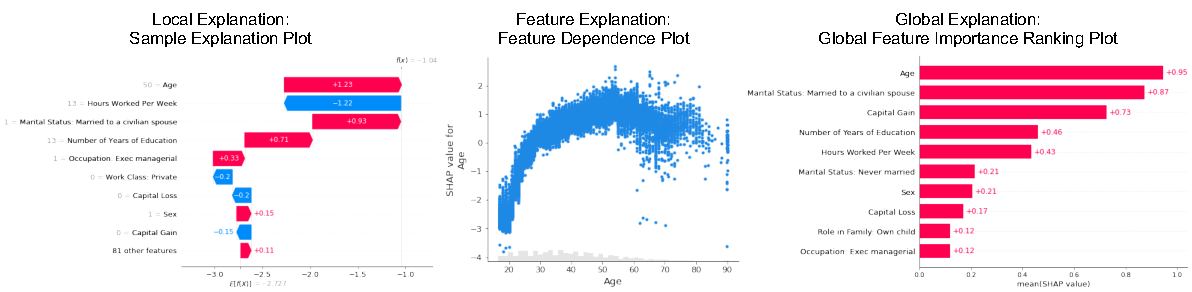
\includegraphics[width=\linewidth, bb=0 0 572 140]{figs/local_to_global.pdf}
    %\captionsetup{width=0.97\textwidth, aboveskip=5pt, belowskip=0pt, singlelinecheck=false}
    \caption{Explanations provided by the SHAP Python package. Left: A
      local explanation for a single data point. Each bar represents a
      single feature's attribution score for that data point. Middle:
      A single feature's attribution scores for all training data
      points, with each data point represented by a dot. Right:
      Global feature attributions obtained by taking the mean absolute
      value of each feature's absolute attribution scores across all
      training data points and then ranking the features by their
      average scores.}
    \label{fig:local_to_global}
\end{figure}

To explore whether ML developers would benefit from being able to
compare and contrast different global feature attributions, we ran an
artifact-based interview study with seven participants who had
experience with interpretability tools.  Participants were first shown
the usual global feature attributions provided by SHAP and asked some
questions about the underlying model.  They were then shown a suite of
global feature attributions obtained by ranking features by four
different summary statistics of their attribution scores---what we
refer to as a global feature attribution suite---and asked to
reconsider their answers.  We note that we do not view the global
feature attribution suite itself as a contribution, but rather as an
artifact for exploring ML developers' perceptions, needs, and
challenges around global feature attributions. Our study addresses the
following research questions:\looseness=-1
\begin{enumerate}
  \setlength\itemsep{0pt} \setlength\parskip{0pt} \item How do ML
  developers make sense of and use global feature attributions
  obtained by ranking features by different summary statistics of
  their attribution scores?
\item Does the ability to compare and contrast different global
  feature attributions allow ML developers to better understand the
  nuanced behavior of models?
\item What challenges do ML developers face when comparing and
  contrasting global feature attributions?
\end{enumerate}

We find that ML developers are able to use different global
feature attributions to achieve tasks and objectives including
communicating what their models have learned and identifying next
steps for debugging their models. Viewing the global feature
attribution suite increased participants' uncertainty in their
understanding of the underlying model (compared with viewing the usual
global feature attributions alone) as they became more aware of the
intricacies of the model's behavior. However, they expressed a tension
between the benefits obtained by using tools like SHAP to quickly get
a sense of what a model has learned and the time it would take to
compare and contrast different global feature attributions. This
tension might limit ML developers' willingness to use a global feature
attribution suite in their own workflows, echoing observations from
prior work about the need to balance the benefits of thinking fast and
thinking slow when designing interpretability
tools~\citep{InterpretingInterpretability}.\looseness=-1

This paper contributes to a recent line of research exploring
human-centered approaches to interpretability. Much of this research
focuses on how stakeholders use and understand interpretability tools
\citep{Lim, Bunt, Bussone, Hohman, Lage, Abdul, Hullman,
  InterpretingInterpretability, Zhang, Poursabzi-Sangdeh,AM21,VW21}.
Within this research, \citet{InterpretingInterpretability} found that
even experienced ML developers tend to misuse and place too much trust
in interpretability tools. They therefore suggested designing
interpretability tools that explicitly highlight the nuanced behavior
of models, as well as methods that counterbalance the bias toward
simple---and potentially misleading---explanations. We see our work as
a first exploration of how one might facilitate deeper understanding
by enhancing overly simplistic global views of a model.



\section{Preliminary Study}
\label{sec:phase1}

To better ground our research, we ran a small preliminary study during
the summer of 2020 to help us understand the current practices of
experienced users of interpretability tools. We conducted
semi-structured interviews with ten ML developers (e.g., data
scientists, research scientists, PhD students) across a variety of
domains (e.g., medicine, finance, retail). Participants were recruited
through a combination of posts to relevant email lists and message
boards at our institution, direct emails to individuals who had
written blog posts or made contributions to either the SHAP Python
package or InterpretML, and snowball sampling.  Each participant had
experience using at least one common interpretability tool, and nine
had experience specifically with SHAP.  Table~\ref{participantTable}
contains additional information about the participants.

During the interviews, we first asked participants about their
background and experience with both ML in general and interpretability
tools in particular. Next, we asked them to describe the
tasks and objectives they use interpretability tools to achieve, both
alone and with collaborators. Participants were asked to walk through
examples of specific times they had used interpretability tools to
accomplish those tasks and objectives, and were led through a series of
open-ended questions intended to uncover the strategies they had used,
including what had worked well and what had not.  Finally,
participants were asked if they had any wishes for a potential new
interpretability tool or for new functionality for an existing
interpretability tool. All interviews were conducted virtually on a
video conferencing platform due to the COVID-19 pandemic.  Audio from
the interviews was recorded and transcribed by a third-party service,
after which the audio transcripts were reviewed for accuracy and
anonymized. The first author then coded the transcripts using a
bottom-up approach and four authors conducted a thematic analysis. The
study was approved by our institution's IRB. Participation was
voluntary and participants received up to \$75 in compensation for
their participation.\footnote{Due to institutional requirements,
  compensation varied based on the relationship between the
  participant and our institution.}

\begin{table}[t!]
  \caption{Descriptions of the participants in our studies.}
  \label{participantTable}
  \begin{tabular}{llllll}
    \toprule
    \bf{ID} & \bf{Job Description} & \bf{\makecell[lt]{Years\\in ML}} & \bf{\makecell[lt]{Types of Data\\Worked With}} & \bf{\makecell[lt]{Interpretability Tools\\ or Methods Used}} & \bf{\makecell[lt]{Study 2\\Dataset}} \\
    \midrule
    P1 & ML PhD Student & 2 & Medical & \makecell[lt]{SHAP, self-made visualizations} & NHANES \\
\hline
    P2 & ML PhD Student & 1 & Medical & \makecell[lt]{InterpretML,
                                        SHAP, LIME, \\ GAMs, self-made visualizations} & NHANES \\
\hline
    P3 & ML Practitioner & 2 & \makecell[lt]{Remote Sensing,\\Retail,
    Banking} & \makecell[lt]{SHAP, self-made visualizations} & N/A \\
\hline
    P4 & \makecell[lt]{Environmental Sci.\\PhD Student}  & 3 & \makecell[lt]{Environmental,\\Geospatial} & \makecell[lt]{SHAP, GAMs,\\self-made visualizations} & N/A \\
\hline
    P5 & Data Scientist & 2 & Retail & SHAP & Adult \\  % P3 in other version
\hline
    P6 & \makecell[lt]{MD and ML PhD\\Student} & 4 & Medical & \makecell[lt]{SHAP, GAMs,\\self-made visualizations} & NHANES \\  % P4 in other version
\hline
    P7 & Research Scientist& 6 & \makecell[lt]{Technology,\\Medical} & \makecell[lt]{SHAP, LIME, GAMs,\\self-made visualizations} & Adult \\ % P5
\hline
    P8 & Data Scientist & 4 & Retail & AzureML, SHAP, LIME & Adult \\
    % P6
\hline
    P9 & \makecell[lt]{Data Scientist,\\Program Manager} & 7 & \makecell[lt]{Retail, Financial,\\User Behavior} & SHAP & N/A \\
\hline
    P10 & ML Practitioner & 3 & \makecell[lt]{Medical,\\Financial} & \makecell[lt]{InterpretML, AzureML, LIME,\\self-made visualizations} & Adult \\ % P7
    \bottomrule
  \end{tabular}
\end{table}

Participants described using interpretability tools for tasks and
objectives including model debugging, improving model performance,
communication and collaboration (including building collaborators'
trust in models), and knowledge discovery.  These tasks and objectives
are very much in line with those identified by \citet{Hullman}. In
total, participants mentioned more than forty different strategies for
accomplishing these tasks and objectives, such as looking for
patterns, outliers, and anomalies in scatter plots of feature
attribution scores for all training data points (as in the middle
panel of Figure \ref{fig:local_to_global}); comparing observed
patterns with prior knowledge; and turning to domain experts when some
aspect of an explanation was unclear.

Strikingly, although our preliminary study was not specifically
designed to explore the use of global feature attributions, all ten
participants said that they use global feature attributions (obtained using
the status quo approach of taking the mean absolute value of each
feature's attribution scores across all training data points and then
ranking the features by their average scores) somewhere in their
workflow.  Participants mentioned using global feature attributions to get an
overall sense of what their models have learned (e.g., for debugging
or for determining the overall credibility of their models), to check
that the ``most important'' features match their expectations, to
determine which features to prioritize for in-depth analysis, and to
communicate what their models have learned to other stakeholders.

However, participants also brought up several pain points around their
use of global feature attributions.  They were aware that using the mean
absolute value could be problematic.  As P2 said, \textit{``ranking of
  feature importance is, you know, a very-- somewhat arbitrary way to
  do things. You know, there's so many different importance
  measures. But, at least looking at something can tell us if our
  model has-- is relying on reasonable features.''}  Some participants
mentioned that using the mean absolute value fails to account for
relatively rare features that have a large influence when they are
present.  Participants also brought up the difficulty of communicating
about the global behavior of models at a level that is more in-depth
than the bar plots that common interpretability tools provide (see the
right panel of Figure \ref{fig:local_to_global}, for example).

Although it wasn't our original focus when we first set out to conduct
this preliminary study, observing participants' overwhelming use of
global feature attributions obtained using the status quo approach in their
workflows---despite being aware of some of the pitfalls---motivated us
to question whether ML developers would benefit from a more nuanced
global view of their models' behavior. That is the question we address
in this paper. Other needs that emerged from the study include ways to
explore and address feature correlation and confounding; less
time-consuming ways to analyze individual features; ways to aggregate
related features to understand their combined influence; ways to
determine the reliability of explanations; ways to validate insights
found using explanations; more customizable visualizations; and
increased documentation for interpretability tools, including
documentation aimed at expert users. We leave these directions for
future work. \looseness=-1





\section{Benefits and Drawbacks of Different Summary Statistics}
\label{sec:background}


In this section, we review the way in which global feature attributions are
most commonly obtained from feature attribution scores, describe some
alternative approaches to doing this, and discuss the benefits and
drawbacks of each. Although most of this discussion is applicable to
any local interpretability method that generates feature attribution
scores, we focus both here and in the rest of this paper on
SHAP~\citep{SHAP} for concreteness.  SHAP's feature attribution
scores, which are motivated by Shapley values from cooperative game
theory, can be viewed as a way of dividing the ``credit'' for a
model's prediction across all of its features.  The sum of the
features' attribution scores is equal to the expected value of the
prediction for the data point in question.  SHAP is widely used in
practice---as of November 2021, the SHAP Python package had close to
15k stars on GitHub, and nine of the ten participants in our
preliminary study had experience with SHAP.

We illustrate the benefits and drawbacks of different approaches to
obtaining global feature attributions from feature attribution scores through
case studies using models trained on two widely used open-source
datasets: the Adult dataset \citep{Adult} and the NHANES dataset
\citep{NHANES}. The Adult dataset is based on 1994 US Census data and
each data point corresponds to a person. The features include age,
employment type, education, marital status, occupation, race, and sex,
among others. The model that we trained on this dataset predicts
whether or not a person makes at least \$50k per year (the equivalent
of about \$92.5k in 2021 when adjusted for inflation). The NHANES
dataset is a survival dataset from a longitudinal health and wellness
study. Again, each data point corresponds to a person. The features
include age, race, sex, poverty index, BMI, lab blood test results,
and blood pressure measurements. The model that we trained on this
dataset is a Cox proportional hazards model that predicts the
differential risk of a person dying versus the typical background risk
(log hazard).

Although SHAP was designed to offer only local explanations, the SHAP
Python package additionally constructs makeshift global feature attributions as
follows: First, for each feature, take the mean absolute value of that
feature's attribution scores across all training data points. Next,
rank the features by their average scores. The resulting global
feature attributions for the models trained on the Adult and NHANES
datasets, respectively, can be seen in the top row of
Figure~\ref{fig:suite}.  For example, according to these global
feature attributions, age is the most important feature for both
models.  This is intuitive since people who are older tend to earn
more money and age is highly correlated with how likely someone is to
die in the near future. But this does not tell the whole story.  For
each of these models, does age play an equal role in the model's
predictions for all training data points, or is it more important for
some data points than for others?  Are there groups of data points for
which the model relies on completely different features?  Are there
outlier data points for which the model relies on features that it
should not?  If the goal is to debug the model, what should the next
step be?


\begin{figure}
    \centering
    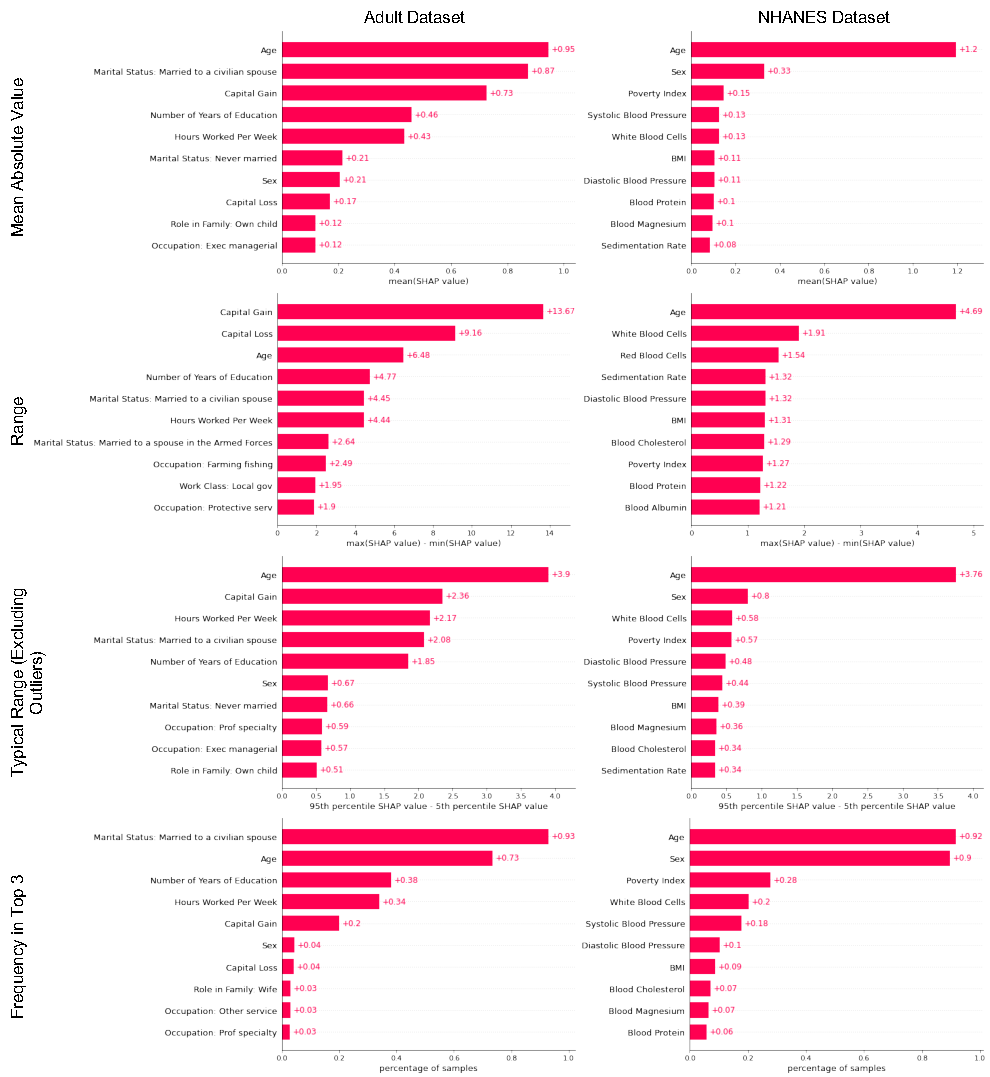
\includegraphics[width=\linewidth, bb=0 0 475 517]{figs/suite.pdf}
    \caption{Global feature attributions obtained by ranking features
      by different summary statistics of their attribution
      scores. Each row corresponds to a summary statistic: the mean
      absolute value, the range, the typical range, and the frequency
      in the top three.  The column on the left contains global
      feature attributions for the model trained on the Adult dataset;
      the column on the right contains global feature attributions for
      the model trained on the NHANES dataset.\looseness=-1}
    \label{fig:suite}
\end{figure}

To answer these questions, an ML developer could turn to a
visualization of a particular feature's attribution score across all
training data points, such as the type of scatter plot shown in the
middle panel of Figure \ref{fig:local_to_global} or the beeswarm plots
available in the SHAP Python package, both of which provide a more
detailed view of a feature's influence. However, for models with
hundreds or even thousands of features, it is too burdensome to
explore and compare all such plots---indeed, this is why developers
turn to summary statistics in the first place.  And even with a small
number of features, comparing plots across multiple features is not
easy.

Instead, we consider supplementing the mean absolute value with other
summary statistics. Using different summary statistics yields
different rankings of the features and, as we show below,
substantively different takeaways. Although in principle any summary
statistic could be used, we propose a few alternatives that capture
different aspects of the distribution of a model's feature attribution
scores across all training data points.\looseness=-1

We first consider the range of a feature's attribution scores---that
is, the difference between the maximum attribution score for that
feature across all training data points and the minimum attribution
score for that feature across all training data points (not taking
absolute values).  Features with a large range of attribution scores
are highly influential on at least some data points.  Outlier data
points can be found by examining scatter plots for features with a
large range.  This is useful both for understanding a model's behavior
on unusual data points and for identifying bugs.  As we can see from
the second row of Figure~\ref{fig:suite}, when predicting whether
someone makes over \$50k a year using the Adult dataset, capital loss
is only the eighth-highest ranked feature when using the mean absolute
value, but the second-highest ranked feature in terms of range. This
is due to extreme outliers---specifically, atypically high capital
loss values---in the training dataset. The prominence of capital loss
in this alternative ranking might help draw a developer's attention to
this issue so they can investigate whether it stems from a bug that
needs fixing or whether it reflects a true phenomenon in the
underlying population.\looseness=-1

In some cases, the range may be too susceptible to outliers. Even a
single data point with an extreme feature attribution score can boost
a feature's range.  This can be problematic if the goal is not to
identify individual outlier data points, but to identify larger groups
of data points for which a feature is highly influential.  As a
result, for this task, it may be more appropriate to use a censored
version of the range.  We define the typical range of a feature's
attribution scores to be the difference between the feature's
ninety-fifth-percentile feature attribution score and its fifth
percentile feature attribution score across all training data
points.\footnote{The choice of the ninety-fifth percentile and the
  fifth percentile is, of course, somewhat arbitrary, and other
  percentiles could be used; we thought that this choice would balance
  the ability to identify groups of data points with robustness to
  extreme outliers.} Ranking features by their typical range can
reveal features that are influential not just for a handful of data
points, but for a more substantial subset of data points. It can
therefore be used to identify groups of data points for which the
model behaves similarly. Examining the second row of
Figure~\ref{fig:suite}, we can see that both red blood cell count and
white blood cell count have a large range for the NHANES model.
However, examining the third row, we can see that only white blood
cell count ranks highly in terms of the typical range. This suggests
that white blood cell count is an important feature for a larger
subset of the training data points than red blood cell count, for
which the large range may be due to outliers.\looseness=-1


The final summary statistic that we consider enables us to get a sense
of which features are influential for a large proportion of the
training data points without worrying about the specific values of
their attribution scores.  We define the frequency in the top three to
be the fraction of the training data points for which the feature in
question ranks among the top three in terms of its absolute feature
attribution scores.  We can think of this as letting every data point
vote for its top three most important features and then tallying up
the votes across the training dataset.\footnote{Again, the choice of
  three votes per data point is arbitrary and other values could be
  used.}  Compared with the mean absolute value, the frequency in the
top three provides a way to control for high variance in the feature
attribution scores.  When predicting whether someone will make over
\$50k a year using the Adult Dataset, the capital gain feature ranks
third in terms of the mean absolute value, and one might therefore
assume it is important for all data points.  However, examining the
final row of Figure~\ref{fig:suite}, we can see that capital gain is
one of the top three most important features for only 20\% of the
training data points. In contrast, hours worked per week is in the top
three for 34\% of the training data points, while its mean absolute
feature attribution score is significantly lower (0.43, compared with
0.73 for capital gain).\looseness=-1


Different summary statistics will yield different global feature attributions
that can be used to derive different---and often
complementary---insights.  We therefore propose that a more accurate
global view of a model's behavior might be achieved by allowing ML
developers to compare and contrast different global feature attributions. In
the next section, we describe a study that we designed to explore this
idea.\looseness=-1


\section{Main Study}

To explore whether ML developers would benefit from being able to
compare and contrast different global feature attributions, we ran a
study in which participants were asked to answer questions about a
model before and after seeing global feature attributions obtained by
ranking features by four different summary statistics of their
attribution scores, as described in Section~\ref{sec:background}. We
refer to this as a global feature
attribution suite, and use it as an artifact for exploring ML
developers' perceptions, needs, and challenges around global feature
attributions.\looseness=-1

\subsection{Methods}

For this study, which we conducted during the summer of 2020, we
recruited seven participants, all of whom had participated in our
preliminary study (see Section~\ref{sec:phase1}) and had agreed to be
contacted for follow-up research; the remaining three participants
declined to participate. The study was approved by our institution's
IRB. Each interview lasted approximately one hour and participants
received a \$50 gift card for their participation.

The study consisted of semi-structured interviews in which
participants were shown two different static (HTML file) Jupyter
notebooks.  Both notebooks contained a model, a textual description of
the dataset used to train the model, a beeswarm plot visualizing the
distribution of attribution scores for each feature, and a feature
dependence scatter plot for each feature (as in the middle panel of
Figure \ref{fig:local_to_global}). In the first notebook, we included
a bar plot showing global feature attributions obtained using the
status quo approach---that is, by taking the mean absolute value of
each feature's attribution scores across all training data points and
then ranking the features by their average scores, as in the top row
of Figure~\ref{fig:suite}---as well as a description of how these
global feature attributions were obtained and a brief list of
potential uses. In the second notebook, we additionally included bar
plots showing global feature attributions obtained using other summary
statistics (specifically, the range, the typical range, and the
frequency in the top three) in addition to the mean absolute value, as
shown in Figure~\ref{fig:suite}. We described how these global feature
attributions were obtained and listed potential uses for each, using
the wording in Table~\ref{tab:descriptions}. All participants were
shown the first notebook before the second notebook. We chose to show
the notebooks sequentially, as opposed to using a counterbalanced
design, so that we could first observe how participants made use of
the usual global feature attributions provided by SHAP, and then see
whether and how their perspectives changed when they were shown the
global feature attribution suite.

\begin{table}[t!]
  \caption{The descriptions of the summary statistics that were shown to participants.}
  \label{tab:descriptions}
  \begin{tabular}{p{0.1\linewidth} p{0.35\linewidth} p{0.47\linewidth}}
    \toprule
    \bf{Statistic} & \bf{How It's Calculated} & \bf{Potential Uses} \\
    \midrule
    Mean Absolute Value & Mean over all samples in the training data set of the absolute value of each sample's model attribution score. & Gives a sense of what the model is learning overall. Currently the default global feature importance ranking in SHAP. \\
\hline
    Range &  Difference between the maximum model attribution score and the minimum model attribution score of the given feature over the training data set. & Identifies features that are heavily influential on at least a small number of samples in the data. Can also help find extreme outliers in the data. \\
\hline
    Typical Range (Excluding Outliers) & Difference between the 95th percentile model attribution score and the 5th percentile model attribution score of the given feature over the training data set. & Identifies features that are heavily influential for at least a substantial subset of samples within the data. More robust to outliers than the Range. Can also help find subsets within the data. \\
\hline
    Frequency in the Top Three & Fraction of samples in the training data set for which the given feature was ranked in the top three in terms of absolute attribution scores.  & Gives a sense of which features most commonly have heavy influence on individual samples' predictions. Can also help to get an understanding without needing to understand the model attribution score. \\
    \bottomrule
  \end{tabular}
\end{table}

To avoid over-indexing on a single dataset or model, we generated
versions of these notebooks for both of the models described in
Section~\ref{sec:background}---that is, the model trained on the Adult
dataset and the model trained on the NHANES dataset.  We assigned the
model trained on the NHANES dataset to the three participants who most
regularly work with medical data and would therefore likely be more
comfortable with both the task and the features; we assigned the model
trained on the Adult dataset to the remaining four participants.
These assignments are listed in the rightmost column of
Table~\ref{participantTable}.

All interviews were conducted virtually on a video conferencing
platform due to the COVID-19 pandemic.  During each interview, the
participant and the interviewer viewed the notebooks together, one at
a time, via screen sharing. The participant had control of the screen
to click, scroll, and explore. Participants were first asked to think
aloud while they familiarized themselves with each notebook. They were
then asked how they would go about accomplishing three of the tasks
and objectives for which participants in our preliminary study had
reported using interpretability tools. Specifically, we asked
participants to describe 1) what they thought the model had learned
overall, 2) how they would explain what the model had learned to
someone who wasn't an ML developer, and 3) what their next steps would
be if they were to go about debugging the model. After completing this
sequence with the first notebook, and then completing it again with
the additional information provided in the second notebook,
participants were asked to share their likes and dislikes for each of
the different global feature attributions, as well as their critical
feedback, the value they gained from using the global feature
attribution suite, and whether they would use a global feature
attribution suite in their own workflows.  The complete notebooks and
the interview protocol can be found at
\url{https://github.com/aokeson/Aggregated-Explainability-Ranking-Alternatives}.

Both audio and video from the interviews was recorded.  Audio was
transcribed by a third-party service, after which the audio
transcripts were reviewed for accuracy and anonymized.  The first
author then annotated each transcript with information about the
visualizations that the participant viewed at different points in time
based on the corresponding video recording. The annotated transcripts
were coded by the first author in three distinct passes: 1) coding
differences in how participants answered our questions when viewing
the first notebook compared with the second notebook, 2) coding
potential uses mentioned by participants for the different global
feature attributions, and finally 3) coding feedback (both positive
and negative) on the global feature attribution suite. All authors
then participated in a thematic analysis using the three types of
codes.

\subsection{Results}
As we describe in this section, participants found the global feature
attribution suite useful for communicating what the model had learned
and identifying next steps for debugging the model. They also found
that it increased their uncertainty in their understanding the model
(compared with viewing the usual global feature attributions alone)
and helped them become more aware of the nuances of the model's
behavior. However, they expressed concerns that the time it would take
to compare and contrast different global feature attributions might
affect the extent to which they would use a global feature attribution
suite in their own workflows.

With our small sample size, we did not see clear differences between
participants who were shown the model trained on the NHANES dataset
and participants who were shown the model trained on the Adult
datasets, so we do not attempt to make distinctions between the two.

\subsubsection{Strategies for Using Different Global Feature Attributions}
Participants used the global feature attributions in a variety of
different ways, exploring them individually as well as comparing and
contrasting different global feature attributions.

Three participants (P5, P6, P7) checked for agreement between the
different global feature attributions in order to pull out specific
features that were influential across more than one of them. This gave
them more confidence that these features were genuinely
influential. For example, P5, who saw the model trained on the Adult
dataset, had named age as being important to the model's predictions
when they viewed the usual global feature attributions provided by
SHAP in the first notebook. After seeing that age was also highly
ranked according to the global feature attributions provided in the
second notebook, they were more confident in their assessment of what
the model had learned and in how to communicate what the model had
learned to other stakeholders, stating \textit{``I would feel rather
  confident that the clearest learning from the model is [...]  around
  age.''} P6 and P7 both independently described this process as
trying to ``flatten'' the different global feature attributions back
to a single list of the most influential features by extracting
features that were highly ranked according to all of the global
feature attributions. \textit{``Maybe you want to start by listing the
  features that are sort of robustly important across an array of
  these different metrics.''} --P6 \looseness=-1

One of the most common strategies for using the global feature
attribution suite was to identify where the different global feature
attributions disagreed and to explore the cause of this
disagreement. Five of the seven participants (P1, P2, P6, P7, and P8)
discussed using this strategy either to uncover new insights into the
model's predictions or as a first step for debugging the model. P7
described going through each feature to check if it was consistently
important, unimportant, or both across the different global feature
attributions: \textit{``Consistently important variables,
  great. Consistently not important variables, great. But variables
  where some trick like that could move you around a lot maybe is
  indicating something. Exactly what, I don't know. But that's why I
  would have to go explore.''} As P6 described, \textit{``It seems
  potentially very useful to come up with several different orderings
  of the features and then try to figure out why those orderings
  disagree in cases where they disagree. That seems like a very
  potentially fruitful way to find either interesting behavior or
  problems with your model.''}  P8, who saw the model trained on the
Adult dataset, also used this strategy.  When looking at the first
notebook, P8 included capital gain in a list of influential features,
because it was among the top three features according to the global
feature attributions obtained using the status quo approach. However,
while exploring the second notebook, P8 found that the different
global feature attributions differed in their rankings of capital gain
and capital loss, and decided to explore this further. They were able
to use this observation to jump start the debugging process by
identifying outliers in the training dataset: \textit{``I think that
  probably the [range] or [typical range] here helps to explain why
  capital gains appears on the [ranking by mean absolute value] but
  rather not in the [ranking by frequency in top three], probably
  because [capital gains] has very high variance and there are some
  outliers in the data, which drags this mean absolute value here. So,
  the outliers are the main cause that drag this capital gain to be
  the top three in [ranking by mean], rather than the [ranking by
    frequency in the top three].''} \looseness=-1

There was no general consensus among participants about which of the
global feature attributions was most appropriate for each of the three
tasks and objectives.  In general, participants followed the brief
guidance that we had provided in the notebooks about potential uses.
For example, P2, who saw the model trained on the NHANES dataset, used
the global feature attributions obtained by ranking features by their
range to identify outliers in the training dataset, saying
\textit{``This range of the blood cell value, so I would want to
  verify that that's a realistic effect, that we're not just picking
  up individuals that have bad values for the white blood cell
  count.''}  In some cases, participants also came up with their own
uses for the different global feature attributions, either
deliberately or by chance. P2, for example, identified a potential bug
in the NHANES dataset after examining the global feature attributions
obtained by ranking features by their frequency in the top three and
then deciding to dig more deeply into the diastolic blood pressure
feature.  \textit{``For instance, there is a group of patients here
  with diastolic blood pressure less than 20. That hardly seems
  realistic. So this is a group of patients for whom either the value
  is missing or it was input wrong.''} --P2

\subsubsection{Increased Uncertainty about the Model's Behavior}

Our hope was that providing ML developers with different global
feature attributions to compare and contrast would lessen their
confidence in the overly simplistic global feature attributions
usually provided by SHAP and instead enable them to obtain a more
nuanced global view of their models' behavior. When interacting with
the first notebook, most participants focused their descriptions of
what the model had learned on a few features that were highly ranked
according to the usual global feature attributions provided by
SHAP. As a result, participants tended to focus their exploration of
the model on a few (typically three to five) features. However, when
exploring the second notebook, participants began to doubt the simple
answers they had given previously.  For example, P7 questioned their
initial interpretation of what the model had learned, saying
\textit{``Now I'm a little hesitant, because I'm not sure. I guess
  there's now four plots, and they are kind of equivalent. [...] So
  now I'm a little confused. I'm not sure which one to trust and to
  use to answer this question.''}  Participants also commented that
their confidence had changed: \textit{``I think it's just sort of
  broadened my confidence intervals on how important each feature
  is.''} \hbox{--P6}.  As desired, participants felt that the global
feature attribution suite provided a more nuanced global view of the
model's behavior than the global feature attributions obtained using
the status-quo approach: \textit{``I mean, it takes you from [...] a
  scalar importance to a distribution of importance. It really helps
  you get that new understanding of how the importance of a feature
  can change over the different samples and the mean will not tell you
  that.''}  --P2 Lastly, participants noted that some of the
information available in the second notebook could be inferred from
other visualizations, such as SHAP's beeswarm plots, but that the new
plots made it easier to digest and interpret the information:
\textit{``I mean, that's similar information for what's in this
  summary plot, but it's condensed in a way that it's much easier to
  read.''} --P2 Indeed, although the distribution of attribution
scores for each feature was available in other plots, this information
was not salient enough to mitigate participants'
overconfidence.\looseness=-1

\subsubsection{Required time investment and constraints} \label{sec:time_investment}

The most common challenge raised by participants was that it might be
too time consuming to compare and contrast different global feature
attributions. P7 articulated a tension between the pressures of
real-world time constraints and the benefits of rigorously examining
multiple global feature attributions: \textit{``And if you are really
  strapped for time, which in the industry you frequently are, then it
  might be easy to just not explore these other things. [...] It makes
  me think that, going forward, I should be a little more vigilant
  about this stuff, but, honestly, it really depends on time.''}
Participants were concerned about whether a global feature attribution
suite would help them accomplish their tasks and objectives more
quickly or instead be yet another time sink.  Participants may have
been overly pessimistic about the time it would take to compare and
contrast different global feature attributions because they were
seeing them for the first time. However, before implementing a global
feature attribution suite in common interpretability tools, more
research is needed to understand how to present different global
feature attributions in the most efficient way possible.

\section{Discussion}

We presented an artifact-based interview study intended to investigate
whether ML developers would benefit from being able to compare and
contrast different global feature attributions. This study extends a
recent line of research exploring human-centered approaches to
interpretability and, in particular, how stakeholders use and
understand interpretability tools~\citep{Lim, Bunt, Bussone, Hohman,
  Lage, Abdul, Hullman, InterpretingInterpretability, Zhang,
  Poursabzi-Sangdeh,AM21,VW21}; however, our focus is on an aspect of
interpretability tools that has been overlooked to date---namely, the
summary statistics used to generate global feature
attributions. Participants were first shown the usual global feature
attributions provided by SHAP and asked some questions about the
underlying model. They were then shown a suite of global feature
attributions obtained by ranking features by four different summary
statistics of their attribution scores---what we refer to as a global
feature attribution suite---and asked to reconsider their answers. Our
hope was that providing ML developers with different global feature
attributions to compare and contrast would lessen their confidence in
the overly simplistic global feature attributions usually provided by
SHAP and instead enable them to obtain a more nuanced global view of
their models' behavior.\looseness=-1

We found that participants were able to use the global feature
attribution suite to communicate what the model had learned and to
identify next steps for debugging the model. As desired, we also found
that viewing the global feature attribution suite increased their
uncertainty in their understanding of the underlying model as they
became more aware of the intricacies of the model's behavior. However,
they also expressed a tension between the benefits obtained by using
tools like SHAP to quickly get a sense of what a model has learned and
the time it would take to compare and contrast different global
feature attributions, noting that this might affect the extent to
which they would use a global feature attribution suite in their own
workflows. Of course, participants were seeing the global feature
attributions for the first time and they only used the global feature
attribution suite for less than an hour. It is possible that with
adequate training and practice, this tension would be reduced or even
overcome. Longitudinal studies may be beneficial for investigating
further. More generally, though, this finding echoes observations from
prior work about the need to balance the benefits of thinking fast and
thinking slow when designing interpretability
tools~\citep{InterpretingInterpretability}.

Like any study, ours has limitations. In addition to the short
timescale over which it was conducted, we only recruited seven
participants. We wanted to be able to conduct an in-depth interview
with each participant about their experiences using the global feature
attribution suite, but this necessarily limits the type of conclusions
that we are able to draw. Furthermore, we focused only on experienced
users of interpretability tools, which further limits the extent to
which we can generalize to the broader ML developer community.  We
also limited our scope to models trained on two datasets, so more
research is needed to investigate whether our findings would change if
different datasets were used---for example, datasets with orders of
magnitude more features. \looseness=-1

We see our work as a first step toward designing interpretability
tools that explicitly highlight the nuanced behavior of models, as
advocated for by \citet{InterpretingInterpretability}. Future work
should explore ways for ML developers to use a global feature
attribution suite to quickly get a sense of what a model has learned
without placing undue confidence in the corresponding global feature
attributions. This will require carefully balancing the cognitive
burden involved in understanding the global feature attributions with
the amount of information that they can convey. It will also require
investigation into which summary statistics to use and which other
information to incorporate. One could imagine, for example,
additionally including other notions of global feature importance,
such as those obtained by applying the concept of Shapley values
directly to global quantities like the variance explained~\citep{OP17}
and the loss~\citep{CLL20} rather than summarizing (local) feature
attribution scores. Doing this well will also require research into
how to present different global feature attributions in the most
efficient way possible.




\section*{Acknowledgments}
We are grateful to members of Microsoft's FATE group and the
  Aether Transparency Working Group---especially Mehrnoosh
  Sameki---for valuable discussions and feedback.


\begin{thebibliography}{10}
\itemsep=1pt
\begin{small}


\bibitem[Abdul et~al.(2020)Abdul, von~der Weth, Kankanhalli, and Lim]{Abdul}
A.~Abdul, C.~von~der Weth, M.~Kankanhalli, and B.~Y. Lim.
\newblock {COGAM}: {M}easuring and moderating cognitive load in machine
  learning model explanations.
\newblock In \emph{Proceedings of the 2020 CHI Conference on Human Factors in Computing
  Systems}, 2020.

\bibitem[Alvarez-Melis et~al.(2021)Alvarez-Melis, Kaur, {Daum\'e III}, Wallach,
  and Vaughan]{AM21}
D.~Alvarez-Melis, H.~Kaur, H.~{Daum\'e III}, H.~Wallach, and J.~W. Vaughan.
\newblock From human explanation to model interpretability: {A} framework based
  on weight of evidence.
\newblock In \emph{AAAI Conference on Human Computation and Crowdsourcing
  (HCOMP)}, 2021.

\bibitem[Barocas et~al.(2021)Barocas, Guo, Kamar, Krones, Morris, Vaughan,
  Wadsworth, and Wallach]{BG+21}
S.~Barocas, A.~Guo, E.~Kamar, J.~Krones, M.~R. Morris, J.~W. Vaughan,
  D.~Wadsworth, and H.~Wallach.
\newblock Designing disaggregated evaluations of ai systems: {C}hoices,
  considerations, and tradeoffs.
\newblock In \emph{Proceedings of the Fourth AAAI/ACM Conference on Artificial
  Intelligence, Ethics, and Society (AIES)}, 2021.

\bibitem[Bunt et~al.(2012)Bunt, Lount, and Lauzon]{Bunt}
A.~Bunt, M.~Lount, and C.~Lauzon.
\newblock Are explanations always important? {A} study of deployed, low-cost
  intelligent interactive systems.
\newblock In \emph{Proceedings of the 2012 ACM International Conference on
  Intelligent User Interfaces}, 2012.

\bibitem[Bussone et~al.(2015)Bussone, Stumpf, and O'Sullivan]{Bussone}
A.~Bussone, S.~Stumpf, and D.~O'Sullivan.
\newblock The role of explanations on trust and reliance in clinical decision
  support systems.
\newblock In \emph{2015 International Conference on Healthcare Informatics},
  2015.

\bibitem[Caruana et~al.(2015)Caruana, Lou, Gehrke, Koch, Sturm, and
  Elhadad]{Caruana2015-qf}
R.~Caruana, Y.~Lou, J.~Gehrke, P.~Koch, M.~Sturm, and N.~Elhadad.
\newblock Intelligible models for {HealthCare} : Predicting pneumonia risk and
  hospital 30-day readmission.
\newblock In \emph{Proceedings of the 21th ACM SIGKDD International Conference
  on Knowledge Discovery and Data Mining}, 2015.

\bibitem[{Centers for Disease Control and Prevention}(1974)]{NHANES}
{Centers for Disease Control and Prevention}.
\newblock {NHANES} data set, 1974.
\newblock Data retrieved from SHAP python package,
  \url{https://github.com/slundberg/shap/tree/master/data}.

\bibitem[Covert et~al.(2020)Covert, Lundberg, and Lee]{CLL20}
I.~Covert, S.~Lundberg, and S.-I. Lee.
\newblock Understanding global feature contributions with additive importance
  measures.
\newblock In \emph{Advances in Neural Information Processing Systems 33}, 2020.

\bibitem[Hastie and Tibshirani(1990)]{hastie1990generalized}
T.~J. Hastie and R.~J. Tibshirani.
\newblock \emph{Generalized Additive Models}.
\newblock CRC Press, June 1990.

\bibitem[Hohman et~al.(2019)Hohman, Head, Caruana, DeLine, and Drucker]{Hohman}
F.~Hohman, A.~Head, R.~Caruana, R.~DeLine, and S.~M. Drucker.
\newblock Gamut: A design probe to understand how data scientists understand
  machine learning models.
\newblock In \emph{Proceedings of the 2019 CHI Conference on Human Factors in Computing
  Systems}, 2019.

\bibitem[Hong et~al.(2020)Hong, Hullman, and Bertini]{Hullman}
S.~R. Hong, J.~Hullman, and E.~Bertini.
\newblock Human factors in model interpretability: Industry practices,
  challenges, and needs.
\newblock \emph{Proceedings ACM Human-Computer Interaction}, 4\penalty0 (CSCW1), 2020.

\bibitem[Jung et~al.(2020)Jung, Concannon, Shroff, Goel, and
  Goldstein]{jung2020simple}
J.~Jung, C.~Concannon, R.~Shroff, S.~Goel, and D.~G. Goldstein.
\newblock Simple rules to guide expert classifications.
\newblock \emph{Journal of the Royal Statistical Society: Series A (Statistics
  in Society)}, 183\penalty0 (3):\penalty0 771--800, 2020.

\bibitem[Kaur et~al.(2020)Kaur, Nori, Jenkins, Caruana, Wallach, and
  Wortman~Vaughan]{InterpretingInterpretability}
H.~Kaur, H.~Nori, S.~Jenkins, R.~Caruana, H.~Wallach, and J.~Wortman~Vaughan.
\newblock Interpreting interpretability: Understanding data scientists’ use
  of interpretability tools for machine learning.
\newblock In \emph{Proceedings of the 2020 CHI Conference on Human Factors in
  Computing Systems}, 2020.

\bibitem[Koh and Liang(2017)]{KL17}
P.~W. Koh and P.~Liang.
\newblock Understanding black-box predictions via influence functions.
\newblock In \emph{Proceedings of the 34th International Conference on Machine
  Learning ({ICML})}, 2017.

\bibitem[Kohavi and Becker(1996)]{Adult}
R.~Kohavi and B.~Becker.
\newblock Adult data set, 1996.
\newblock Data retrieved from SHAP python package,
  \url{https://github.com/slundberg/shap/tree/master/data}.

\bibitem[Lage et~al.(2019)Lage, Chen, He, Narayanan, Kim, Gershman, and
  Doshi-Velez]{Lage}
I.~Lage, E.~Chen, J.~He, M.~Narayanan, B.~Kim, S.~J. Gershman, and
  F.~Doshi-Velez.
\newblock Human evaluation of models built for interpretability.
\newblock In \emph{AAAI Conference on Human Computation and Crowdsourcing
  (HCOMP)}, 2019.

\bibitem[Lim and Dey(2011)]{Lim}
B.~Y. Lim and A.~K. Dey.
\newblock Investigating intelligibility for uncertain context-aware
  applications.
\newblock In \emph{Proceedings of the 13th International Conference on
  Ubiquitous Computing}, 2011.

\bibitem[Lundberg and Lee(2017)]{SHAP}
S.~M. Lundberg and S.-I. Lee.
\newblock A unified approach to interpreting model predictions.
\newblock In \emph{Advances in Neural Information Processing Systems 30}, 2017.

\bibitem[Nushi et~al.(2018)Nushi, Kamar, and Horvitz]{Nushi2018}
B.~Nushi, E.~Kamar, and E.~Horvitz.
\newblock Towards accountable {AI}: {H}ybrid human-machine analyses for
  characterizing system failure.
\newblock In \emph{AAAI Conference on Human Computation and Crowdsourcing
  (HCOMP)}, 2018.

\bibitem[Owen and Prieur(2017)]{OP17}
A.~B. Owen and C.~Prieur.
\newblock On {S}hapley value for measuring importance of dependent inputs.
\newblock \emph{SIAM/ASA Journal on Uncertainty Quantification}, 51\penalty0 (1):\penalty0 986--1002, 2017.

\bibitem[Poursabzi-Sangdeh et~al.(2021)Poursabzi-Sangdeh, Goldstein, Hofman,
  Wortman~Vaughan, and Wallach]{Poursabzi-Sangdeh}
F.~Poursabzi-Sangdeh, D.~G. Goldstein, J.~M. Hofman, J.~W. Wortman~Vaughan, and
  H.~Wallach.
\newblock Manipulating and measuring model interpretability.
\newblock In \emph{Proceedings of the 2021 CHI Conference on Human Factors in Computing
  Systems}, 2021.

\bibitem[Quinlan(1986)]{quinlan1986induction}
J.~R. Quinlan.
\newblock Induction of decision trees.
\newblock \emph{Maching Learning}, 1\penalty0 (1):\penalty0 81--106, 1986.

\bibitem[Ribeiro et~al.(2016)Ribeiro, Singh, and Guestrin]{LIME}
M.~T. Ribeiro, S.~Singh, and C.~Guestrin.
\newblock "{W}hy should {I} trust you?": {E}xplaining the predictions of any
  classifier.
\newblock In \emph{Proceedings of the 22nd {ACM} {SIGKDD} International
  Conference on Knowledge Discovery and Data Mining}, 2016.

\bibitem[Robinson(1950)]{R50}
W.~S. Robinson.
\newblock Ecological correlations and the behavior of individuals.
\newblock \emph{American Sociological Review}, 15\penalty0 (3):\penalty0
  351--357, 1950.

\bibitem[Rudin(2019)]{rudin2019please}
C.~Rudin.
\newblock Stop explaining black box machine learning models for high stakes
  decisions and use interpretable models instead.
\newblock \emph{Nature Machine Intelligence}, 1\penalty0 (5):\penalty0
  206--215, 2019.

\bibitem[Russell(2019)]{R19b}
C.~Russell.
\newblock Efficient search for diverse coherent explanations.
\newblock In \emph{Proceedings of the Conference on Fairness, Accountability,
  and Transparency ({FAT*})}, 2019.

\bibitem[Ustun et~al.(2019)Ustun, Spangher, and Liu]{USL19}
B.~Ustun, A.~Spangher, and Y.~Liu.
\newblock Actionable recourse in linear classification.
\newblock In \emph{Proceedings of the Conference on Fairness, Accountability,
  and Transparency ({FAT*})}, 2019.

\bibitem[Vaughan and Wallach(2021)]{VW21}
J.~W. Vaughan and H.~Wallach.
\newblock A human-centered agenda for intelligible machine learning.
\newblock In M.~Pelillo and T.~Scantamburlo, editors, \emph{Machines We Trust:
  Perspectives on Dependable AI}. MIT Press, 2021.

\bibitem[Weld and Bansal(2019)]{WB19}
D.~S. Weld and G.~Bansal.
\newblock The challenge of crafting intelligible intelligence.
\newblock \emph{Comm. of the ACM}, 62\penalty0 (6):\penalty0 70--79, 2019.

\bibitem[Zeng et~al.(2017)Zeng, Ustun, and Rudin]{zeng2017interpretable}
J.~Zeng, B.~Ustun, and C.~Rudin.
\newblock Interpretable classification models for recidivism prediction.
\newblock \emph{Journal of the Royal Statistical Society: Series A (Statistics
  in Society)}, 180\penalty0 (3):\penalty0 689--722, 2017.

\bibitem[Zhang et~al.(2020)Zhang, Muller, and Wang]{Zhang}
A.~X. Zhang, M.~Muller, and D.~Wang.
\newblock How do data science workers collaborate? {R}oles, workflows, and
  tools.
\newblock \emph{Proceedings ACM Human-Computer Interaction}, 4\penalty0 (CSCW1), 2020.


\end{small}
\end{thebibliography}


%\bibliographystyle{abbrvnat}
%{\small
%\bibliography{bib}
%}


\end{document}

\end{article}
%
%\makeatletter
%\renewcommand{\AB@affillist}{}
%\renewcommand{\AB@authlist}{}
%\setcounter{authors}{0}
%\makeatother
%
\begin{article}
{``Mixture of amazement at the potential of this technology and concern about possible pitfalls'': Public sentiment towards AI in 15 countries}
{Patrick Gage Kelley, Yongwei Yang, Courtney Heldreth, Christopher Moessner, Aaron Sedley, and Allison Woodruff}
\graphicspath{{submissions/Woodruff_final/}}
%\documentclass[11pt,dvipdfm]{article}
\documentclass[11pt]{article} %The above line must be used for your camera-ready submission, which requires a latex -> DVI -> PDF compilation pipeline.  As a workaround while you are writing your paper, you could comment it out and use this line instead, which is compatible with pdflatex.

%\documentclass[conference,onecolumn]{IEEEtran}
% \IEEEoverridecommandlockouts
% The preceding line is only needed to identify funding in the first footnote. If that is unneeded, please comment it out.
\usepackage{deauthor,times}


%\usepackage{tabularx}
\usepackage{booktabs}
%\usepackage[super]{nth}     % for easier ordinal number
\usepackage{enumitem}     % better lists
\usepackage{url}
\usepackage{hyperref}
\usepackage{multicol}
\usepackage{footnote}
%\usepackage{cite}
\usepackage{graphicx}
\usepackage{xcolor}
\def\BibTeX{{\rm B\kern-.05em{\sc i\kern-.025em b}\kern-.08em
    T\kern-.1667em\lower.7ex\hbox{E}\kern-.125emX}}
    
%\usepackage{amsmath,amssymb,amsfonts}
%\usepackage{algorithmic}
%\usepackage{textcomp}

\definecolor{darkgray}{RGB}{100,100,100}
\definecolor{darkplum}{RGB}{50,10,50}
\definecolor{Mahogany}{RGB}{103,10,10}
\definecolor{RedInstruct}{RGB}{180,45,45}

% QUOTE AFFILIATIONS
\newcommand\aff[1]{\textcolor{darkplum}{{\emph{--#1}}}}

% QUESTION LABELS
% flip the next two lines to turn on and off question labels
% \newcommand\q[1]{\textcolor{Mahogany}{\small{\textbf{[#1]}}}}
  \newcommand\q[1]{\textcolor{Mahogany}{\small{\textbf{}}}}

% tables for grayness
\newcommand\graynew[1]{\textcolor{darkgray}{#1}}

% FORMATTING FOR OUR QUOTE LISTS

\newenvironment{lq2}
{ \vspace{-3pt}
  \begin{itemize}[leftmargin = 4.0em, rightmargin=5.0em, label={}]
    \fontsize{10pt}{10.7pt}\selectfont
    \setlength{\itemsep}{3pt}
    \setlength{\parskip}{2.5pt}
    \setlength{\parsep}{3pt}     }
{ \end{itemize} \vspace{1pt}  }

% FORMATTING FOR OUR QUOTE LISTS IN THE FIGURE PAGE

\newenvironment{lq1}
{ \begin{itemize}[leftmargin = 0em, label={}]
    \fontsize{8pt}{8.6pt}\selectfont
    \setlength{\itemsep}{2pt}
    \setlength{\parskip}{2pt}
    \setlength{\parsep}{2pt}       }
{ \end{itemize}                    }

% MACRO FOR GROUP LABELS

 \def\Exciting/{{\fontfamily{lmss}\selectfont\textbf{Exciting}}}  \def\Useful/{{\fontfamily{lmss}\selectfont\textbf{Useful}}}
 \def\Worrying/{{\fontfamily{lmss}\selectfont\textbf{Worrying}}}
 \def\Futuristic/{{\fontfamily{lmss}\selectfont\textbf{Futuristic}}}
 \def\None/{{\fontfamily{lmss}\selectfont\textbf{None}}}

%\newcommand{\highlight}{\cellcolor{lightgray}}

% MACROS FOR QUESTIONS IN THE SUPPLEMENT
% \newcommand\question[1]{\bigskip\noindent\textcolor{darkgray}{\large{\textbf{#1}}}\newline}
\newcommand\question[1]{\bigskip\noindent\textcolor{darkgray}{{\textbf{#1}}}\newline}
\newcommand\sample[1]{\noindent\{\textcolor{RedInstruct}{#1}\}\newline}
\newcommand\questiontext[1]{\noindent{#1}}
\newcommand\openend{\\[2pt]\indent\{Open-end\}}





\begin{document}
\title{``Mixture of amazement at the potential of this technology and concern about possible pitfalls'': Public sentiment towards AI in 15 countries}
\author{
  Patrick Gage Kelley,* Yongwei Yang,* Courtney Heldreth,* \\
  Christopher Moessner,$\dagger$ Aaron Sedley,* Allison Woodruff* \vspace{0.2cm}\\ 
  ~*\textit{Google} \\
        \fontfamily{pcr}\selectfont\small
        \href{mailto:patrickgage@acm.org}{patrickgage@acm.org},
        \href{mailto:yongwei@google.com}{yongwei@google.com},
        \href{mailto:cheldreth@google.com}{cheldreth@google.com}, \\ 
        \fontfamily{pcr}\selectfont\small
        \href{mailto:asedley@google.com}{asedley@google.com}, 
        \href{mailto:woodruff@acm.org}{woodruff@acm.org} \vspace{0.2cm}\\
  $\dagger$\textit{Ipsos}\\
        \fontfamily{pcr}\selectfont\small
        \href{mailto:christopher.moessner@ipsos.com}{christopher.moessner@ipsos.com}}





\maketitle

\begin{abstract}
Public opinion plays an important role in the development of technology, influencing product adoption, commercial development, research funding, career choices, and regulation. In this paper we present results of an in-depth survey of public opinion of artificial intelligence (AI) conducted with over 17,000 respondents spanning fifteen countries and six continents. Our analysis of open-ended responses regarding sentiment towards AI revealed four key themes (exciting, useful, worrying, and futuristic) which appear to varying degrees in different countries. These sentiments, and their relative prevalence, may inform how the public influences the development of AI.

\end{abstract}

%\begin{IEEEkeywords}
%artificial intelligence, public opinion, survey research
%\end{IEEEkeywords}

\section{Introduction}
Increased understanding of the societal impact of artificial intelligence (AI) has spurred strong interest its in responsible development~\cite{dietterich2015rise,hawking2014,horvitz2012interim, stone2016artificial}.
Researchers, advocates, companies, and others have proposed processes, principles, design toolkits, and other resources to support thoughtful development of AI that carefully considers both benefits and risks~\cite{abrassart2018, fjeld2020, highlevel2019,jobin2019,scuEthics,googleAI,princetonEthics,ethicalOS}.

Public opinion is an important force in responsible development, exerting pressure on funding agencies, regulators, companies, educators, and others to address both general attitudes and specific issues~\cite{castro2019, cave2018portrayals,ouchchy2020,zhang2022}, such as the impact of automation on the future of work~\cite{brynjolfsson2014second, raghavan2020, sanchez-mondero2020},  the interaction of AI with human rights issues such as privacy and discrimination~\cite{abrassart2018, barabas2018, buolamwini2018, chancellor2019}, the ethics of autonomous weapons~\cite{scharre2018army, west2018}, and the development and availability of dual-use technologies such as synthetic media that may be used for either benevolent or nefarious purposes~\cite{openAI2019}. While public opinion may not fully align with expert assessment on these issues, it is nonetheless useful to elucidate the forces in effect.

 While there have been some explorations of public perception of AI, for example, survey research~\cite{arm2017, blumberg2019, cave2019, ipsos2019, mozilla2019, northeastern2018, west2018, zhang2019artificial}, sentiment analysis~\cite{chuan2019, fast2017long, garvey2019sentiment, ouchchy2020}, and narrative analysis~\cite{cave2018portrayals, cave2020narratives}, much of this work has been done in Western, English-speaking contexts. Even in these better studied contexts, much remains to be learned, as both the technology and the public discussion are evolving rapidly. In this paper, we present a survey of public perception of AI conducted with over 17,000 respondents spanning fifteen countries and six continents (encompassing in total: Germany, Australia, Finland, Singapore, Belgium, Canada, the United States (US), South Korea, Spain, France, Poland, Brazil, China, India, and Nigeria). Using an inductive approach to analyze open-ended responses, we identified four key sentiment groups (exciting, useful, worrying, and futuristic) whose prevalence distinguishes responses to AI in different countries. We previously shared results from eight of these countries~\cite{kelley2021} and here we extend our analysis to fifteen countries and more fully discuss the sentiments. We then discuss implications of these findings for the development of AI systems. 

\section{Background}
Artificial intelligence (AI) is a broad term with no consensus definition~\cite{edelman2019, fast2017long, stone2016artificial},
and the scope of our inquiry is intended to be similarly broad.
We note that interpretation of the term is further confounded by the ``AI effect'' (the phenomenon that once AI successfully solves a problem and the solution becomes commonplace, it is no longer considered to be AI)~\cite{mccorduck2004machines}, as well as lack of awareness of algorithmic processing in common systems~\cite{eslami2015always, rader2015understanding, warshaw2016intuitions}. 
To aid comparison with survey responses,
following~\cite{stone2016artificial}, we share with the reader the following definition provided by Nils J. Nilsson: ``Artificial intelligence is an activity devoted to making machines intelligent, and intelligence is the quality that enables an entity to function appropriately and with foresight in its environment.''~\cite{nils2009}

\subsection{Empirical Studies}
Much of the research on public perception of AI has been survey-based, often conducted in Western, English-speaking countries such as the US and the UK~\cite{blumberg2019, cave2019, edelman2019, zhang2019artificial, northeastern2018} although this has been broadening recently.
AI is often viewed as likely to have a significant impact on the future, with a frequent expectation that its effects will be positive.
In a 2019 Edelman survey in the US, 9 out of 10 respondents assumed that AI will be life-changing and transformational~\cite{edelman2019}.
A Gallup survey conducted in the US in 2018 found that 76\% believed that AI will have a positive impact on their lives~\cite{northeastern2018}; 61\% of respondents had a positive view of AI and robots in a large-scale 2017 survey across Europe on the impact of digitization and automation on daily life~\cite{european2017}; and a 2017 consumer research survey conducted across North America, Europe, and Asia revealed a predominant expectation that society will become better (61\%) rather than worse (22\%) due to increased automation and AI~\cite{arm2017}. A recent Pew Research survey conducted across the Americas, Europe, and Asia showed a somewhat narrower margin (possibly due to shifting public opinion, or alternatively, methodological differences), with a median of 53\% saying that AI has been mostly good for society (53\%) versus mostly bad (33\%)~\cite{funk2020}. Considering expected impact in the next 20 years, the 2019 World Risk Poll indicated AI would mostly help (41\%) versus mostly harm (30\%) people in one's own country, with more favorable impressions in Asia and less favorable impressions in Western countries~\cite{lloyds2020, neudert2020}.

At the same time, AI is neither interpreted as exclusively beneficial nor exclusively disadvantageous, and public response often indicates contradictory emotions. Looking at broad reactions, Blumberg reported that US respondents were equally split between feeling optimistic and informed and feeling fearful and uninformed about AI~\cite{blumberg2019}, while~\cite{arm2017} also revealed both excitement and concern. Relatedly, a 2019 Mozilla survey open to respondents on the Internet gathered continent-level demographic data and revealed varying and mixed emotions at the continent-level~\cite{mozilla2019}. Specific concerns have been expressed regarding social issues, such as AI benefiting the wealthy and harming the poor, fear that AI-enabled deepfakes will erode trust in information, and AI increasing social isolation and reducing human capability~\cite{edelman2019}. In line with these concerns, Zhang and Dafoe found that 82\% of Americans want AI and robots to be carefully managed~\cite{zhang2019artificial}, with 88\% of Europeans expressing similar sentiment~\cite{european2017}. Moreover, 60\% of the general population in the Edelman survey expressed the need for more regulation regarding AI development and deployment~\cite{edelman2019}.

Qualitative work has also explored public perception of algorithmic systems, for example, finding that perception of algorithmic systems can vary substantially by individual factors as well as platform~\cite{devito2017platforms}, and that end users often have fundamental questions or misconceptions about technical details of their operation~\cite{bucher2017algorithmic, eslami2015always, rader2015understanding, ur2012smart, warshaw2016intuitions}.

\subsection{Narratives and Media Sentiment Analysis}
AI is not only heavily discussed in academia, but is also a popular topic in public media and entertainment~\cite{edelman2019}. In fact, Cave et al. provide a history of narratives about intelligent machines dating back to ancient Greece~\cite{cave2020narratives}. In modern times, 58\% of the respondents in a recent Blumberg survey indicated that they get information about AI from movies, TV, and social media~\cite{blumberg2019}. In a 2016 CBS news survey, only 19\% indicated not having seen any of several AI movies such as ``The Terminator'' or ``I, Robot''~\cite{cbs2016}. Cave et al. argue that prevalent AI narratives in the English-speaking West share ``a tendency towards utopian or dystopian extremes,'' cautioning that inaccurate narratives could affect technological advancement and regulation~\cite{cave2018portrayals}, with similar points raised in~\cite{horvitz2012interim, stone2016artificial, you2015}. Cave et al. surveyed UK respondents regarding their responses to eight dominant narratives about AI, reporting that the strong majority elicited more concern than excitement~\cite{cave2019}.

At the same time, while some researchers have argued that narratives and fiction may be disproportionately frightening, studies have suggested that news reports may be more balanced or appropriately critical. Sentiment analysis of newspaper articles from the New York Times and associated content found that, in general, AI has had consistently more optimistic than pessimistic coverage over time~\cite{fast2017long}, and did not support the hypothesis that news media coverage of AI is negative~\cite{garvey2019sentiment}. Content analysis of coverage of AI in five major American newspapers revealed benefits were discussed more frequently than risks, although risks were discussed with greater specificity~\cite{chuan2019}. Ouchchy et al. analyzed discussion of AI ethics in English language media sources and concluded that ``The issues most frequently covered, along with the mostly balanced/neutral tones, suggest that the media has a fairly realistic and practical focus in its coverage of the ethics of AI.''~\cite{ouchchy2020}

\subsection{National Considerations}
A number of countries have established national strategies to promote the use and development of AI, which vary by country and may influence public perception~\cite{dutton2018}.\footnote{See also \url{https://futureoflife.org/national-international-ai-strategies/}} 
The importance of studying local context is also illustrated by analysis of country-specific opportunities and challenges for AI, e.g.~\cite{kalyanakrishnan2018opportunities}.
Further, researchers have called for better integration of developing country considerations in the discussion and development of AI~\cite{sambasivan2019toward}.

\subsection{Our Approach}
Our work sits within a growing body of research on people’s perceptions of AI, across disciplines including HCI, critical studies, law, marketing, policy, psychology, and more. This topic is highly complex, multi-dimensional, and far from fully understood. Methodologically, this means that techniques such as \textit{triangulation} (studying the same phenomenon from multiple vantage points, in order to cross-check and more fully capture richness and complexity, e.g. using both qualitative and quantitative methods to see if the findings are consistent)~\cite{salkind2010} and \textit{replication} (the reproduction and extension of prior work)~\cite{wilson2014} are particularly useful for this topic. Accordingly, we seek to broaden and enrich the understanding of sentiment towards AI by looking for emergent themes in a large number of open-ended responses from a wide range of countries.


\section{Methodology}
In order to better understand public perception of AI, 
we partnered with Ipsos, a global market research firm, 
to conduct a survey of 17,014 respondents in fifteen countries in July and December 2019.\footnote{For logistical reasons we split data collection into two rounds: July 2019 (Australia, Canada, US, South Korea, France, Brazil, India, and Nigeria) and December 2019 (Germany, Finland, Singapore, Belgium, Spain, Poland, and China). Based on our experience with similar surveys and our knowledge of world events at the time, we do not expect the time interval between the two rounds had a substantial impact on the results.}
Methodologically, this work falls in the genre of public opinion polling, as described below.

\subsection{Instrument Development and Translation}
To develop concepts and questions, we consulted experts at our institutions, reviewed published work, drew on our own previous unpublished research, and conducted an initial pilot survey in June 2018 with 1300 respondents drawn from a panel of the general online population in the US. Many questions in the final instrument were written uniquely for this survey while others were modified from or replicate other questions in the literature or the canon of public opinion surveys. In order to more accurately reflect real-world settings, we did not define AI, and left interpretation of the term to the respondents.\footnote{We note that in our pilot, we had two versions of the survey (one that defined AI and one that did not) and responses to subsequent questions were similar regardless of whether a definition had been provided.} We included primarily closed-form questions as well as a few open-ended questions for free responses. We also included standard demographic questions such as age, gender, education, income, region, and urbanicity. The final instrument included several dozen questions on a range of topics related to artificial intelligence (for more information, see the Appendix). 

After we completed the instrument in English, we engaged cApStAn, a linguistic quality assurance agency with expertise in survey translation. We made several improvements based on their insights to minimize terminology that would be difficult to translate. In consultation with cApStAn, we also developed a translation style guide to ensure consistency and address complexities for particular concepts and/or languages. Our market research partner's in-country translation teams and/or third party vendors then translated the full instrument to all target languages while referring to the style guide. See Table~\ref{tab:demographics} for the languages we offered. After the survey was complete, the responses were provided to the coding team to be coded in-language as described below. Illustrative quotes in this paper are verbatim (in the case of English language responses) or were prepared or reviewed by professional translators (in the case of non-English language responses).

\subsection{Deployment}
We selected a range of countries with different characteristics, such as stage of technological development, nature of the workforce, and varied development indices. The survey was fielded to online panels (groups of respondents who have agreed to participate in surveys over a period of time) representative of the online population in each country. Consistent with the best panels available for online market research, such panels tend to be broadly representative of the general population in countries with high access to technology, but less representative of the general population in countries with more limited access to technology; for example, in developing countries they tend to skew urban. Respondents were recruited using stratified sampling (a method of recruiting specific numbers of participants within demographic subgroups), with hard quotas on age and gender in each country. A summary of countries and demographics is provided in Table~\ref{tab:demographics}.\footnote{For compact layout, in all tables we use standard two-letter country codes, which are shown with full country names in Figure~\ref{fig:venn}.}\textsuperscript{,}\footnote{The alert reader may notice the gender differences in India and Nigeria. Percentages were chosen to match benchmarks of the gender distribution of the online population in each country.}
% Germany (DE), Australia (AU), Finland (FI), Singapore (SG), Belgium (BE), Canada (CA), United States (US), South Korea (KR), Spain (ES), France (FR), Poland (PL), Brazil (BR), China (CN), India (IN), Nigeria (NG)




\begin{table*}[t!]
\centering
\small

\begin{tabularx}{1.01\textwidth}{@{}l XXXXXXXX@{}}

\emph{Country}	& \bf 	DE	& \bf 	AU	& \bf 	FI	& \bf 	SG	& \bf 	BE	& \bf 	CA	& \bf 	US	&	 \bf KR	\\
\midrule
{HDI Rank}	    &	\nth{6}	& \nth{8}	& \nth{11}	&	\nth{11}	& \nth{14}  &	\nth{16}	& \nth{17}  &	\nth{23} \\
\midrule
{Languages}	&	German	&	English	&	Finnish	&	Chinese,	&	Dutch,	&	English,	&	English	&	Korean	\\
{offered}	    &	    	&		    &	    	&	English	    &	French	&	French	    &		    &		    \\

\midrule
{Weighting}    
                    & \scriptsize age, \newline gender, \newline education, \newline region
                    & \scriptsize age, \newline gender, \newline education, \newline region
                    & \scriptsize age, \newline gender, \newline education, \newline region
                    & \scriptsize age, \newline gender, \newline education
                    & \scriptsize age, \newline gender, \newline education, \newline region
                    & \scriptsize age, \newline gender, \newline education, \newline region
                    & \scriptsize age, \newline gender, \newline education, \newline region, race
                    & \scriptsize age, \newline gender, \newline education, \newline region \\

\specialrule{0.1em}{4pt}{3pt}
																	
{Respondents}	&	1002	&	1000	&	1002	&	1000	&	1000	&	1500	&	1501	&	1000	\\
\footnotesize \emph{(n) All} \\
																	
\midrule
{Gender} 	&	51\% \tiny{men}	&	49\% \tiny{men}	&	48\% \tiny{men}	&	54\% \tiny{men}	&	54\% \tiny{men}	&	47\% \tiny{men}	&	49\% \tiny{men}	&	52\% \tiny{men}	\\
 	&	49\% \tiny{women}	&	51\% \tiny{women}	&	52\% \tiny{women}	&	47\% \tiny{women}	&	46\% \tiny{women}	&	53\% \tiny{women}	&	51\% \tiny{women}	&	48\% \tiny{women}	\\
																	
\midrule
%\emph{Age}	&	43.7	&	42.8	&	41.0	&	39.6	&	40.5	&	44.0	&	43.6	&	39.4	\\
Age\footnotesize{, avg.}	&	44	&	43	&	41	&	40	&	41	&	44	&	44	&	39	\\
\scriptsize{Age, stddev}	&	\scriptsize 15.4	&	\scriptsize 15.3	&	\scriptsize 15.2	&	\scriptsize 12.7	&\scriptsize 	15.1	&\scriptsize 	16.0	&	\scriptsize 17.5	&\scriptsize 	12.4	\\

\bottomrule																	
	& & \\																	& & \\	
		& & \\																

\emph{Country}	    & \bf ES	& \bf FR	& \bf PL	& \bf BR	    & \bf CN	& \bf IN	    & \bf NG			\\
\midrule
{HDI Rank}	    & \nth{25}	& \nth{26}	& \nth{35}	& \nth{84}	    & \nth{85}	& \nth{131}	    & \nth{161}			\\
\midrule
{Languages}	&	Spanish	&	French	&	Polish	&	Brazilian	&	Chinese	&	English,	&	English		\\
{offered}	    &		    &	    	&	    	&	Portuguese	&   		&	Hindi	    &				\\

\midrule
{Weighting}    
                    & \scriptsize age, \newline gender, \newline education, \newline region
                    & \scriptsize age, \newline gender, \newline education, \newline region
                    & \scriptsize age, \newline gender, \newline education, \newline region
                    & \scriptsize age, \newline gender, \newline education, \newline region
                    & \scriptsize age, \newline gender, \newline education, \newline region
                    & \scriptsize age, \newline gender, \newline education
                    & \scriptsize age, \newline gender, \newline education \\

\specialrule{0.1em}{4pt}{3pt}
																	
{Respondents}	&	1002	&	1001	&	1000	&	1503	&	1003	&	1500	&	1000			\\
\footnotesize \emph{(n) All} \\
																	
\midrule
Gender	&	52\% \tiny{men}	&	50\% \tiny{men}	&	50\%  \tiny{men}	&	49\% \tiny{men}	&	53\% \tiny{men}	&	70\%  \tiny{men}	&	63\% \tiny{men}			\\
&	48\% \tiny{women}	&	50\% \tiny{women}	&	50\% \tiny{women}	&	51\% \tiny{women}	&	47\% \tiny{women}	&	30\% \tiny{women}	&	37\% \tiny{women}			\\
% \emph{Male}	&	51.9\%	&	50.0\%	&	50.3\%	&	49.0\%	&	53.4\%	&	70.1\%\footnotemark	&	63.1\%			\\
% \emph{Female}	&	48.1\%	&	50.0\%	&	49.7\%	&	51.0\%	&	46.6\%	&	29.9\%	&	36.9\%			\\


\midrule
Age\footnotesize{, avg.}	&	42	&	43	&	41	&	34	&	38	&	30	&	31			\\
%\emph{Age}	&	42.3	&	42.6	&	40.5	&	34.2	&	38.2	&	29.9	&	30.7			\\
\scriptsize{Age, stddev}	&	\scriptsize 12.9	&	\scriptsize 15.4	&	\scriptsize 14.1	&	\scriptsize 12.3	&	\scriptsize 12.0	&	\scriptsize 8.9	& \scriptsize 	9.0			\\

\bottomrule
\vspace{0.01cm}

\end{tabularx}

\caption{ Country details, respondent summary and demographics. All numbers unweighted. }
\label{tab:demographics}

\end{table*}

% SK really is 39 years of age (more precisely, 39.4), although the AIES paper says 40





The median survey length was 21.4 minutes across all completions, including those who said they had never heard of AI in an early screening question and received a much shorter version of the survey. All respondents received incentives in a point system or cash at an industry-standard amount for their market.

\subsection{Data Processing and Analysis}

\subsubsection{Quality Checks}
The market research firm conducted quantitative and qualitative checks to remove low quality responses on an ongoing basis until the quota was reached in each country. Example grounds for removal included being identified as a bot, speeding (answering substantially more quickly than the median time), or providing nonsensical or profane responses to open-ended questions.

Overall we removed 6.1\% of responses for quality. After data collection was complete, standard procedures were followed to apply a modest weighting adjustment to each respondent so that the samples in each country are more representative~\cite{biemer2008weighting}. 
This weighting is reflected in the data shared in Section~\ref{Sec:Results}. The variables considered in weighting appear in Table~\ref{tab:demographics}.

\subsubsection{Research Objective and Data}
In this paper we focus on the following research objective: What sentiment do respondents have towards AI? Specifically, we present emergent themes, descriptive statistics, and illustrative quotes for the following open-ended question about sentiment: 

\begin{itemize}
\item[] \textit{`What feelings or emotions come to mind when you hear the phrase Artificial Intelligence (AI)?'}
\end{itemize}

When we present illustrative quotes, we also draw on responses from three additional open-ended questions (about description of AI, examples of AI, and any uncomfortable experiences with AI), as relevant responses and similar coding often applied across all of the open-ended questions.\footnote{The first question about sentiment was shown to all respondents, while the remaining three questions were only shown to respondents who reported that they had heard of AI before the survey.}

\subsubsection{Coding and Analysis of Open-Ended Responses}\label{Coding_Section}
We reviewed the open-ended responses from the pilot to identify emergent themes~\cite{beyer1997contextual} and develop an initial codebook for all questions, then iterated as we reviewed responses from all countries to refine it as necessary.
The open-ended responses were coded by our market research partner's dedicated coding team or one of their third party coding vendors. The coding was done in the source language, with the exception of Dutch and Finnish which were coded based on English translations.
As described in McDonald et al., a variety of different approaches may be employed to improve the reliability of qualitative analysis~\cite{mcdonald2019}.
In our case, following best practices in public opinion research for coding against multiple languages, we used professional coders, followed an iterative process to continuously improve the codes, and performed a series of hierarchical quality checks.
While coders were specialized by language, they worked together to ensure consistency, sharing notes in specialized coding software. Both we and our market research partner performed multiple levels of quality checks on the resulting coding, randomly sampling from all responses in each country as well as checking all instances of select codes. 

We used an inductive approach to explore emerging themes and common patterns in the data~\cite{hinkin1998brief}. For the open-ended question regarding the feelings or emotions the respondent associated with AI, we began by following the process described above; the resulting codebook for this question encompassed 92 codes (e.g. `Useful,' `Skeptical,' `AI takes over') and specified that multiple codes could be assigned per response. After these codes were assigned and we reviewed the open-ended verbatim responses in detail, four thematic groups of codes emerged from the data as common and semantically distinct: \Exciting/, \Useful/, \Worrying/, and \Futuristic/. For example, the \Useful/ group encompassed codes such as `Useful,' `Helpful,' `Productivity,' etc. We assigned each of the 92 codes to exactly one of these four sentiment groups or Other accordingly. Other encompassed answers that were inarticulate, classified as unable to be coded, mentions of technology without any sentiment (e.g. ``computer" or ``technology"), and a long tail of other opinions on AI (for example ``curiosity" or ``surprise"). Based on the codes that each response had been assigned, each response was considered to be part of those group(s) -- for example, if a response had been assigned the code `Helpful' and the code `Concern,' that response was part of the sentiment groups \Useful/ and \Worrying/. A response that received \textit{only} codes labeled Other appears in \None/.

\subsubsection{Human Development Index}\label{HDI_Section}
As the impact and use of AI expands worldwide, how people learn about, interact with, and use AI varies. People from developed countries (i.e. countries that are more industrialized and have higher per capita incomes, for example, Germany, Australia, Finland, or Singapore) have different circumstances than people from developing countries (i.e. countries that are less industrialized and have lower per capita incomes, for example, Brazil, China, India, and Nigeria), and this shapes how AI is perceived, adopted, and normalized globally~\cite{un2014, sambasivan2019toward}. Therefore, we anticipated that there might be meaningful differences in AI perceptions associated with development level. We include the Human Development Index (HDI) Rank in Table~\ref{tab:demographics}.\footnote{We show HDI ranks from the 2020 Human Development Report \url{http://hdr.undp.org/en/2020-report}, which uses HDI values from 2019, aligning with the dates of our survey deployment.}

\subsection{Limitations}

We note several limitations of our methodology that should be considered when interpreting this work. First, it carries with it the standard issues attendant with survey methodology, such as the risk of respondents misunderstanding questions, poor quality translation, or respondents satisficing~\cite{holbrook2003telephone} or plagiarizing open-ended responses. We have worked to minimize these risks through piloting, use of open-ended questions in conjunction with closed-form questions, use of a translation style guide and translation review, and data quality checks. We also note that panels in India are well-known in the industry to be disproportionately likely to have a social desirability response bias (as defined in~\cite{holbrook2003telephone}), so optimism in the responses from India should be considered in that context. Second, online panels are not representative of the general population. While we have used a high standard of currently available online panels, we caveat our findings as not representative of the general population, particularly in Brazil, China, India, and Nigeria. Third, while members of the research team and/or market research partner team have experience conducting research in all markets studied, members of the team reside in Western countries. We have worked to minimize the risk of misinterpretation by collaboration and discussion with in-country partner teams but recognize that our interpretations may lack context or nuance that would have been more readily available to local residents.




\section{Results}\label{Sec:Results}
In this section we describe the sentiment groups that emerged from our analysis and present data on the frequency of their occurrence. Responses to the open-ended sentiment question were assigned to groups as described in Section~\ref{Coding_Section}. Many responses were brief and were assigned only one code, for example, responses such as ``exciting'' or ``robot'' would be assigned \Exciting/ or \Futuristic/, respectively. However, responses were often more lengthy and received multiple codes. For example, a response such as ``fear and excited at the same time'' (US respondent) would be included in \Worrying/ and \Exciting/, but not \Useful/ or \Futuristic/.

\begin{figure*}[p]
\centering
\vspace{-0.7cm}
  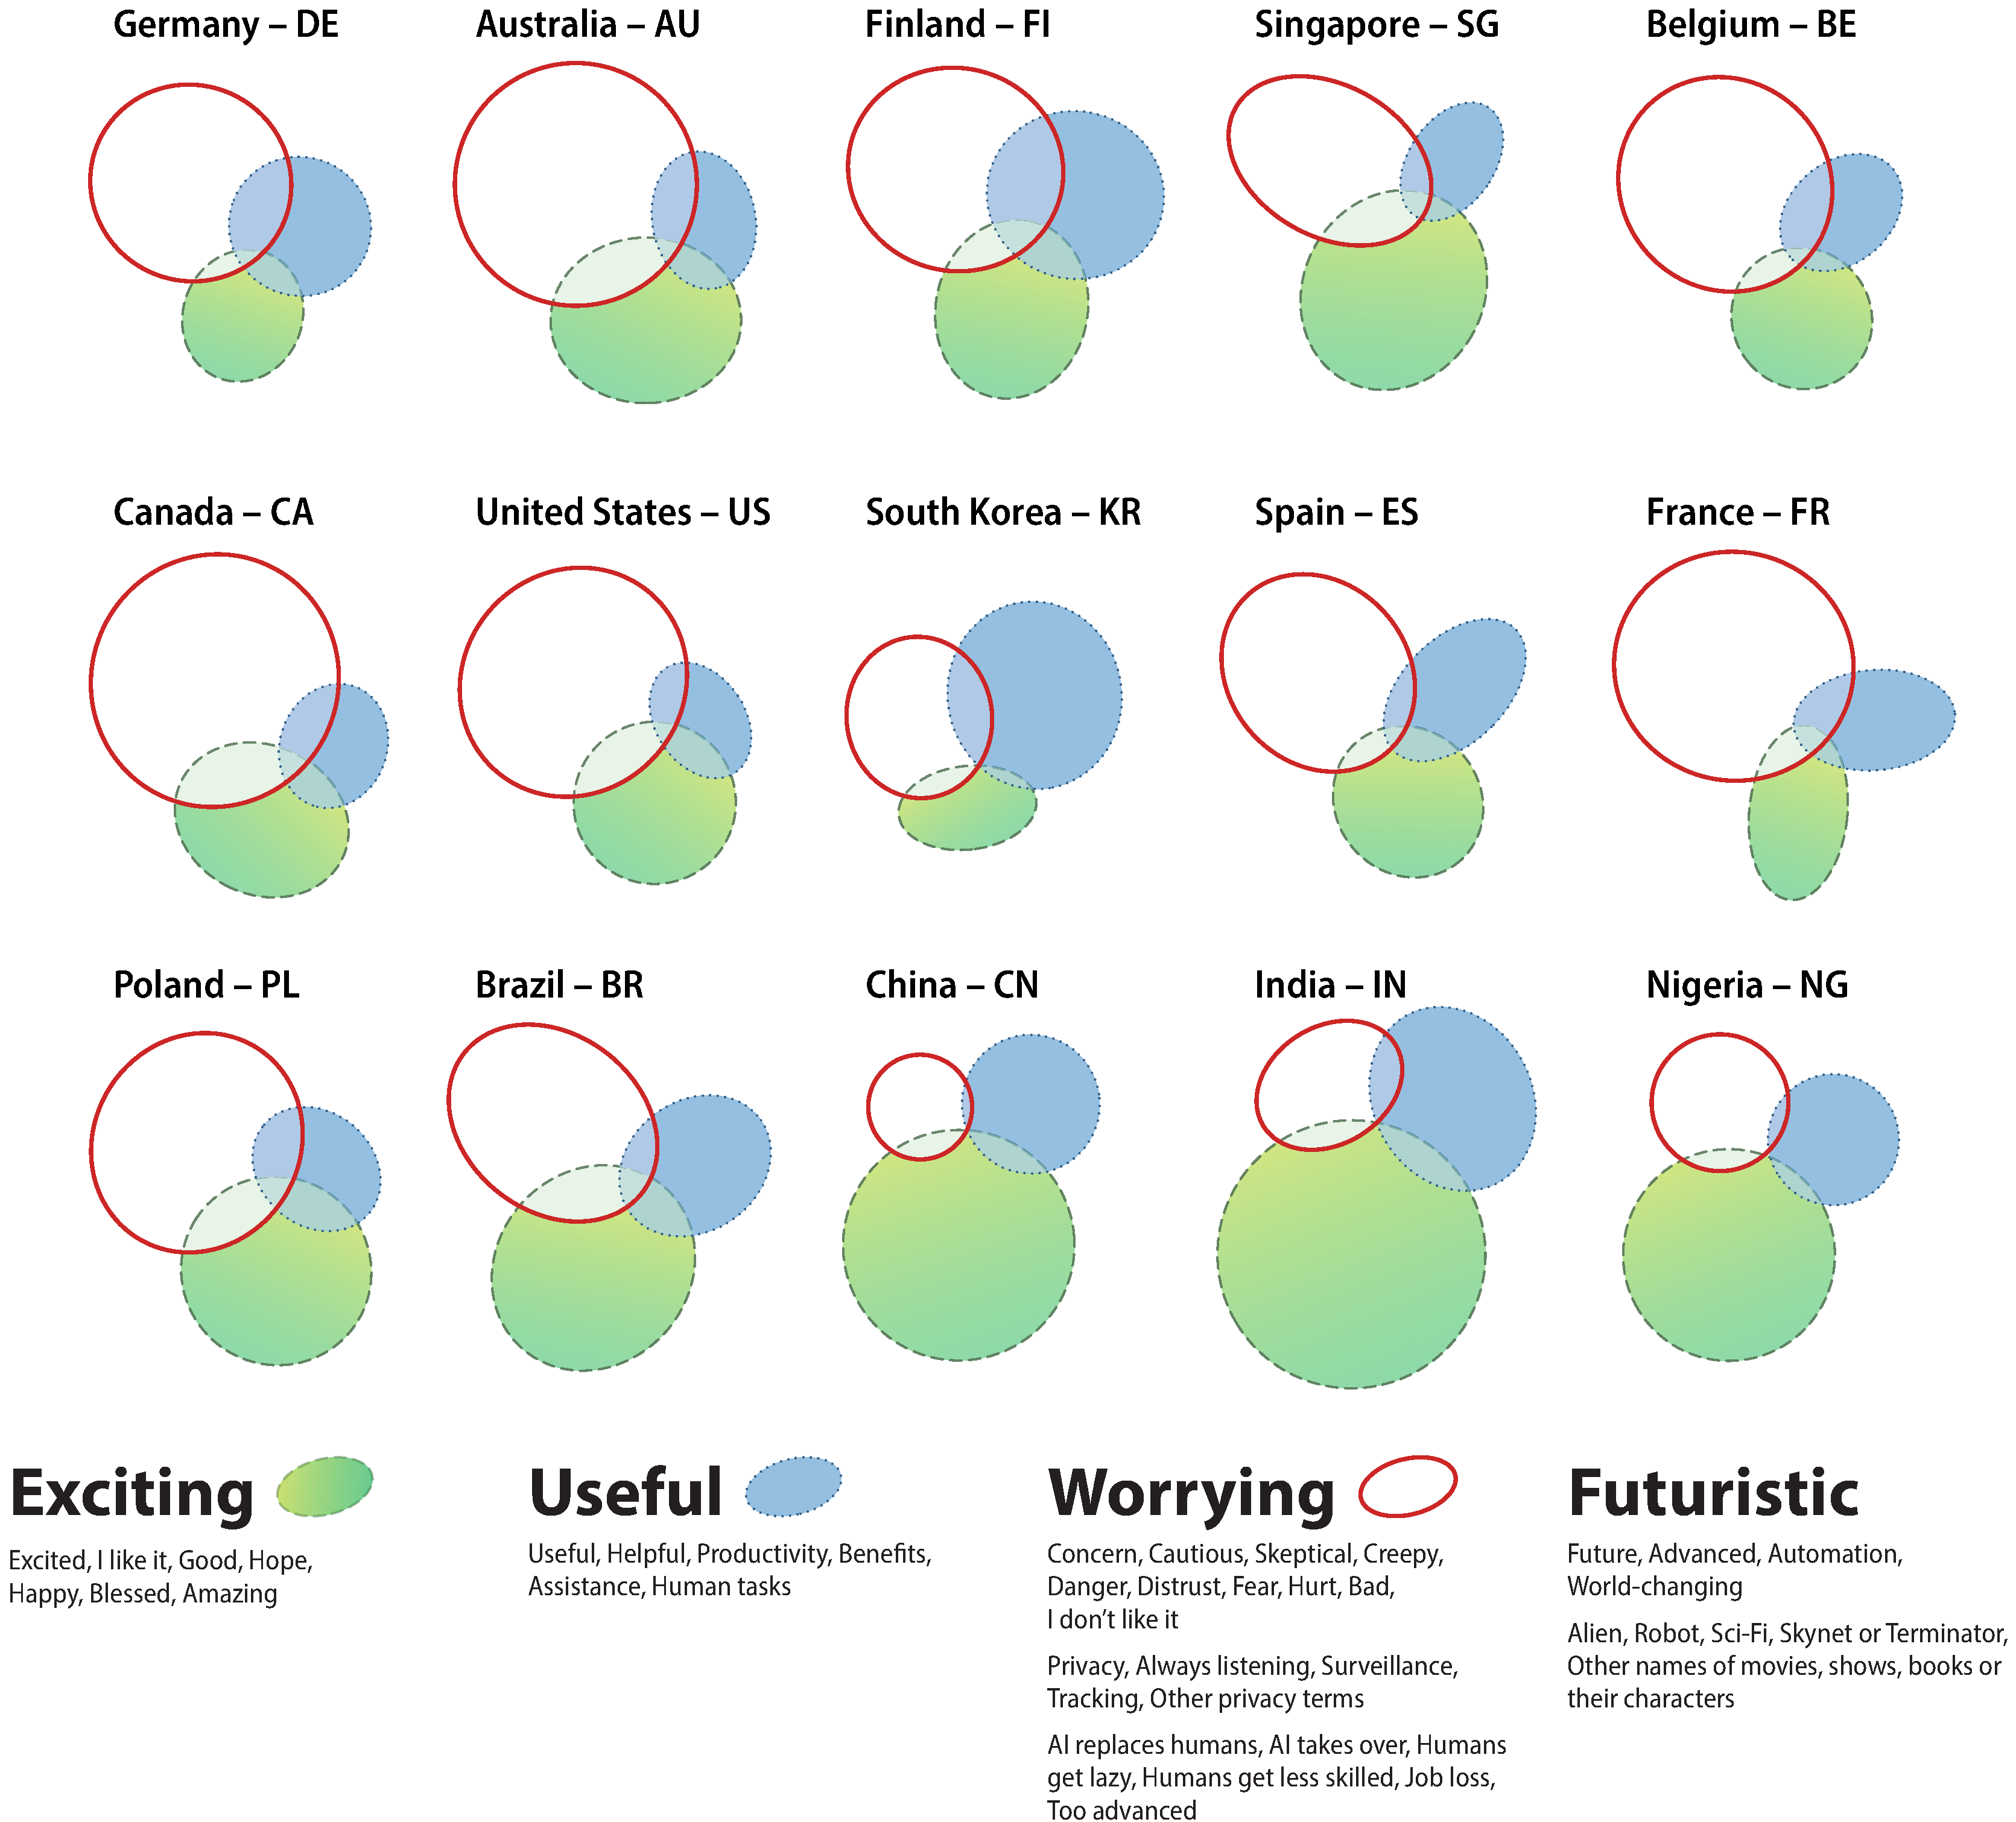
\includegraphics[width=0.95\textwidth]{figs/Rplot09.pdf}
\vspace{-0.3cm}
\setlength\columnsep{12pt}
\begin{multicols}{4}

% EXCITING

\begin{lq1}
%\item \Exciting/
\item excitement for what it can do to simplify and enrich our lives \aff{Canada}
\item Amazing technology that helps us out with everyday mundane things. \aff{US}
\item Happiness, joy from the heart, is to feel that life is convenient \aff{China}
\item joy! The future is now! \aff{Belgium}
\item Happy when I hear this word this can change entire world \aff{India}
\item Great feelings, like the world is moving into a new realm \aff{Nigeria}
% \item I am glad that I am living in a time of such progress. I have high hopes for the development of AI. \aff{Poland}
\end{lq1}

\columnbreak

% USEFUL
\begin{lq1}
%\item \Useful/
\item I have a good feeling! This technology can become useful. \aff{Brazil}
\item A robot that can make people's life more convenient \aff{South Korea}
\item A helpful assistant that is there for us and assists with daily tasks \aff{US}
\item Destined to improve our lives, robotic technology \aff{Spain}
\item Positive, something that makes our lives easier \aff{Poland}
\item The next big efficient thing for humans. \aff{Nigeria}
\end{lq1}

\columnbreak

% WORRYING
\begin{lq1}
%\item \Worrying/ 
\item It is interesting and useful, but I am worried about lost jobs, not to mention AI getting smart enough to take over and control us. \aff{Canada}
\item A little bit of fear because I don't know the limit of Artificial intelligence (if there is a limit) \aff{Nigeria}
% \item This topic is thought-provoking. It generates fear and also curiosity and concern. \aff{Brazil}
\item Progress but danger. Fear, uncertainty. \aff{France}
\item No no no, will ruin everything \aff{Finland}
\item Fearful of our future robot overlords \aff{Australia}
\end{lq1}

\columnbreak

% FUTURE figure
\begin{lq1}
%\item \Futuristic/ (not pictured)
\item Artificial intelligence is the future. It will bring the dawn of a new age \aff{Nigeria}
\item It is the technology that forms the foundation of lives in the next century. \aff{Singapore}
\item A dystopian future, in a way. \aff{Finland}
\item This is the future, personally I don't think it's developing well \aff{Germany}
% \item I try to make an effort to follow this futuristic trend. I really like it and I am onboard with AI in general sense. \aff{Brazil}
\item its magnificient technology of tomorrow \aff{India}
\end{lq1}

\end{multicols}

  \vspace{-0.4cm}
  \caption{\small{Description of our four sentiment groups, with the complete list of codes that comprises each, and example responses. While we use the responses to illustrate a particular sentiment, some of them fall in multiple sentiment groups, as sometimes occurred in our data set. At the top of the figure, we represent the overlap between the groups with Venn diagrams, using 3-Venn diagrams which exclude Futuristic for readability. The alert reader may wonder why we use oblong circles; these more accurately represent the area in the overlap. We use the method described in \protect\cite{micallef2014eulerape}. Countries are ordered by HDI.}}
  \label{fig:venn}
\end{figure*}


Figure~\ref{fig:venn} and Table~\ref{tab:sentimentgroups} present the prevalence of sentiment groups in each country. We now discuss each sentiment in turn.


\subsection{Exciting}

Responses in this group contained positive feelings about AI and often exhibited broad excitement or enthusiasm. These feelings were often direct statements of excitement, but also included other positive feelings such as joy or a sense of feeling blessed to have AI. \Exciting/ sentiment was often associated with a sense of newness or expectation of substantial change. Sometimes respondents expressed excitement about improvements in daily life, and sometimes they anticipated broad improvement for humanity.

\begin{lq2}
\item Excited to see where this tech goes in future, hope to see AI assist with everyday life in the home and in work \aff{Australia}\footnote{Throughout the paper, we share complete verbatim responses (in some cases translated) and do not correct typographic or grammatical errors. The only exception is the quote in the title, which is a verbatim excerpt from a response that is shared in full in Section~\ref{Mixed_Section}.}
\item Happiness, because it means humanity moves forward. \aff{Spain}
\item A bit of excitement, fascination, curiosity, but also somewhere deep a feeling of uncertainty, a thrill related to the effect that it may have on my future, however, that is mostly due to the influence of film rather than a result of conscious assessment of the benefits that AI will bring. \aff{Poland}
\end{lq2}

Some respondents were also excited about potential economic advantages for their country, and a few mentioned personal career opportunities that AI might provide.


\begin{table*}[t]\centering
% \ra{1.3}
\footnotesize
\begin{tabular}{@{}l@{\hskip 0.3cm}rrrrrrrrrrrrrrr@{}}

\emph{Country} & \bf DE & \bf AU & \bf FI & \bf SG & \bf BE & \bf CA & \bf US & \bf KR & \bf ES & \bf FR & \bf PL & \bf BR & \bf CN & \bf IN & \bf NG \\

\midrule
Respondents  & 1002 & 1000 & 1002 & 1000 & 1000 & 1500 & 1501 & 1000 & 1002 & 1001 & 1000 & 1503 & 1003 & 1500 & 1000 \\
($n$) \graynew{\emph{All}} \\
\midrule
\Exciting/ &     9\% & 17\% & 14\% & 22\% & 12\% & 14\% & 15\% &  6\% & 14\% & 10\% & 25\% & 23\% & 28\% & 36\% & 25\% \\
\Useful/ &      12\% &  9\% & 17\% &  7\% &  9\% &  9\% &  7\% & 19\% & 13\% & 11\% & 13\% & 14\% & 13\% & 17\% & 11\% \\
\Worrying/ &    23\% & 31\% & 25\% & 20\% & 27\% & 33\% & 30\% & 14\% & 23\% & 31\% & 30\% & 21\% &  7\% & 9\% &  11\% \\
\Futuristic/ &  17\% & 22\% & 24\% & 21\% & 15\% & 21\% & 19\% & 38\% & 28\% & 20\% & 22\% & 34\% & 24\% & 24\% & 19\% \\
\None/ &        48\% & 38\% & 36\% & 38\% & 48\% & 39\% & 42\% & 31\% & 34\% & 39\% & 32\% & 25\% & 37\% & 27\% & 41\% \\

\bottomrule
\vspace{0.01cm}

\end{tabular}
% \captionof{table}{
\caption{Weighted percentage of respondents from each country whose open-ended sentiment was coded to be in one of our groups. Respondents can appear in multiple sentiment groups. A respondent whose answers received only codes not in these groups appears in \None/.}
\label{tab:sentimentgroups}

\end{table*}

% India really is 17\% useful, even though the AIES paper says 18\%


\subsection{Useful}
Responses in this group expressed the belief that AI will be helpful and assist humans in completing tasks. \Useful/ sentiment was generally associated with practical implications of AI. For example, respondents spoke of AI improving productivity in industrial settings. They also spoke of AI providing personal convenience, making people's lives easier and more comfortable, assisting with daily life, enabling smart home technology, and helping people perform mundane tasks.

\begin{lq2}
\item It is a kind of high technology that brings great convenience to our lives. \aff{China}
\item A tool of the future to make everyday life easier \aff{Finland}
\item Replaces man in thankless tasks \aff{Belgium}
\end{lq2}

Respondents also spoke of AI helping humanity by addressing large societal issues such as healthcare or the environment.
\begin{lq2}
\item Really interesting. Hopefully it can solve energy issues and other large problems. \aff{Finland}
\item Progress, I know it will impact positively especially in the areas of health care.~\aff{Nigeria}
\end{lq2}

\subsection{Worrying}
Many respondents shared that AI is \Worrying/, causing them concern, fear, or anxiety. Unlike the previous two groups, which each capture a relatively tight set of responses to AI in our open-ended data, this group comprises a wide range of negative emotional responses.
\begin{lq2}
\item Do we need that? It scares me! \aff{Germany}
\item A dangerous game. \aff{Finland}
\item It's progress, but I am not sure that it is so positive for society \aff{Belgium}
\end{lq2}

While some respondents spoke of general concerns, many spoke to specific aspects of AI they found \Worrying/. For example, some respondents were concerned that AI might challenge humans and take over society. Sometimes they suggested that popular culture had caused this concern. Correspondingly, they sometimes also spoke to the need for humans to control AI.
\begin{lq2}
\item A threat to the future of humanity. \aff{Finland}
\item regret, it will make work and then the world disappear \aff{Belgium}
\item Can improve or end our lives. \aff{Germany}
\item A mixture of knowledge and fear. I know that it will help or is already helping in several important areas, but there is always that fear that one of these AIs will become too autonomous and turn against us.~\aff{Brazil}
\item That was always coming. But because of all those films on TV with the AI, I still have my reservations. I mean you never know, right? \aff{Belgium}
\item Does no one watch movies, read, or anything to do with science fiction!!! It ALWAYS ends badly... there is just no good outcome, that I can see (for now at least), to an actual, fully fledged, AI.~\aff{US} 
\end{lq2}

Respondents also saw privacy concerns as a likely downside of AI. Sometimes they mentioned privacy in broad terms, but they often raised specific concerns such as worrying that products constantly listen to them, or concerns about being surveilled in the workplace.
\begin{lq2}
\item A new frontier. Very exciting and scary at the same time. Lots to gain but will personal privacy be the price?~\aff{Australia}
\item Could lead to total surveillance \aff{Germany}
\item A trending mobile app that undresses people. It violates privacy rules~\aff{Nigeria}
\item IT DICTATED MY WEIGHT AND HEIGHT IN PUBLIC.~\aff{India}
\item Installing a monitoring system in the office makes people very uncomfortable \aff{China}
\item Ads that show up on computers after visiting websites is one thing, but ads that show up after just talking about something makes me think my phone is listening in on my conversations~\aff{US}
\item The phone's microphone recognizes speech and this information is used in marketing. Should I dare speak about sensitive matters near the phone at all \aff{Finland}
\end{lq2}

Respondents expected that AI would negatively impact the number of jobs available in the future. They perceived that AI may replace humans or make them less necessary in the workforce, and particularly  associated robots with job loss due to their ability to perform human tasks. In rare cases, respondents shared personal experiences with automation-related job loss.
\begin{lq2}
\item I feel that it has taken away jobs~\aff{US}
\item A highly computerised potentially dangerous job stealing system of machinery operation~\aff{Australia}
\item New technologies. Convenience in life. Reduction in jobs.~\aff{South Korea}
\item Am happy about it but am still sceptical about it. This is because it might probably put some persons out of work~\aff{Nigeria}
\item Unemployment comes to my mind when I hear the phrase Artificial Intelligence(AI).~\aff{India}
\end{lq2}

Respondents also expressed concern that humans will become over-reliant on AI and become lazy, or that AI will minimize human contact and negatively impact personal relationships in the future.

\begin{lq2}
\item This is a futuristic innovation that can help people but also make them too lazy~\aff{Nigeria}
\item fear that during my lifetime I will be interacting more with AI than live humans~\aff{US}
\item It helps the future by making things easier, but diminishes employment and human contact.~\aff{France}
\end{lq2}

\subsection{Future}
Although \Futuristic/ may not traditionally be seen as a sentiment, when we asked respondents to describe their feelings or emotions about AI, they organically responded at very high rates and it was clearly a strong association
(15\% to 38\% across the countries).
Responses in this group are not necessarily positive or negative towards AI,
but rather are included for any mention of the futuristic nature of AI, whether by simply describing AI as advanced; mentioning robots, aliens, or other science-fiction concepts; or by referencing the future directly.

Some respondents who spoke of the future expressed that AI will be transformative, for example saying that it will usher in a new era and profoundly change society.
\begin{lq2}
\item Something new. Something that will change the world \aff{Poland}
\item AI can change every aspect of human life. \aff{Singapore}
\item we are entering a new era. Very modern~\aff{Canada}
\item AI will revolutionise the way we live in our future.~\aff{India}
\end{lq2}

The expected future effects of AI were sometimes described as \Exciting/, \Useful/, \Worrying/, or some combination of these. We discuss mixed feelings further below.
\begin{lq2}
\item A thing of the future that is sure to be of great use! \aff{Finland}
\item Better future \aff{Spain}
\item A big problem for humanity in the future. \aff{Poland}
\item Machines taking over humans!! :) on a serious note, A.I. is making things possible we thought were not possible a few years ago. Computers recognise faces and fingerprints of humans. Machines carry out so many things to assist humans. Everywhere we look there are examples of artificial intelligence around us.~\aff{Australia}
\item AI is the new trend for technology, I myself being a tech geek i know that AI is soon going to change the whole world with it's endless possibilities. AI is the future of Mankind \aff{India}
\end{lq2}




\begin{table*}\centering
\footnotesize
\begin{tabular}{@{}l rrrrr rrrrr rrrrr @{}}

Country	&	\bf DE	&	\bf AU	&	\bf FI	&	\bf SG	&	\bf BE	&	\bf CA	&	\bf US	&	\bf KR	&	\bf ES	&	\bf FR	&	\bf PL	&	\bf BR	&	\bf CN	&	\bf IN	&	\bf NG		\\
	
	\midrule
												
Respondents 	&	1002	&	1000	&	1002	&	1000	&	1000	&	1500	&	1501	&	1000	&	1002	&	1001	&	1000	&	1503	&	1003	&	1500	&	1000				\\
	($n$) \graynew{\emph{All}} \\
	\midrule
													
Neutral	&	31\%	&	24\%	&	9\%	&	24\%	&	28\%	&	26\%	&	27\%	&	14\%	&	25\%	&	25\%	&	21\%	&	11\%	&	28\%	&	9\%	&	9\%	\\
I don't know 	&	16\%	&	17\%	&	19\%	&	5\%	&	19\%	&	15\%	&	9\%	&	8\%	&	15\%	&	17\%	&	8\%	&	11\%	&	1\%	&	4\%	&	3\%	\\
Other	&	12\%	&	7\%	&	10\%	&	6\%	&	9\%	&	7\%	&	10\%	&	14\%	&	12\%	&	9\%	&	11\%	&	9\%	&	9\%	&	15\%	&	19\%	\\
Inarticulate	&	15\%	&	5\%	&	12\%	&	10\%	&	12\%	&	7\%	&	6\%	&	4\%	&	6\%	&	19\%	&	8\%	&	4\%	&	7\%	&	7\%	&	4\%	\\
Curious	&	3\%	&	9\%	&	8\%	&	6\%	&	5\%	&	7\%	&	6\%	&	2\%	&	10\%	&	5\%	&	22\%	&	16\%	&	16\%	&	5\%	&	7\%	\\
Intelligence	&	1\%	&	4\%	&	5\%	&	9\%	&	6\%	&	3\%	&	7\%	&	10\%	&	5\%	&	2\%	&	3\%	&	9\%	&	7\%	&	13\%	&	18\%	\\
Technology	&	3\%	&	4\%	&	6\%	&	2\%	&	2\%	&	6\%	&	5\%	&	5\%	&	7\%	&	3\%	&	3\%	&	12\%	&	11\%	&	11\%	&	10\%	\\
Fake	&	1\%	&	3\%	&	4\%	&	3\%	&	4\%	&	4\%	&	7\%	&	3\%	&	2\%	&	1\%	&	4\%	&	2\%	&	0\%	&	6\%	&	17\%	\\
Computer	&	3\%	&	4\%	&	5\%	&	6\%	&	3\%	&	4\%	&	7\%	&	4\%	&	2\%	&	3\%	&	2\%	&	5\%	&	1\%	&	5\%	&	6\%	\\
Device	&	1\%	&	3\%	&	4\%	&	4\%	&	1\%	&	3\%	&	2\%	&	12\%	&	3\%	&	2\%	&	3\%	&	3\%	&	1\%	&	9\%	&	6\%	\\

\bottomrule
\vspace{0.01cm}
\end{tabular}

\caption{ The 10 most common codes within the \None/ group, which includes all respondents who were assigned none of the codes in our four sentiment groups. Weighted percentages indicate how many respondents within the \None/ group were assigned a given code, by country. }
\label{tab:nones}

\end{table*}




\subsection{None}
The groups above do not cover all responses.
Some responses were assigned only the 49 codes that we did not include in our sentiment groups, in which case they fell into the \None/ group described in Section~\ref{Coding_Section}.
These included, for example, broad mentions of technology (responses such as ``technology'' or ``computer''). See Table~\ref{tab:nones}.

\subsection{Mixed Feelings}\label{Mixed_Section}
As seen above, a given response sometimes contained multiple sentiments toward AI. In some responses, these were all positive sentiments, for example, excitement that AI would be helpful in daily life. However, a number of responses were more ambivalent. Sometimes such responses contrasted specific positive expectations (e.g. personal convenience or improved healthcare) with specific negative expectations (e.g. reduced privacy or job loss). Additionally, these mixed emotions were sometimes coupled with a sense of resignation or inevitability. 

\begin{lq2}
\item It is a wonderful and terrifying concept that is inevitable.~\aff{Australia}
\item The future of our world in a way that represents both progress and destruction~\aff{Canada}
\item optimistic that it will enhance peoples lives and bring about breakthroughs in many fields but also skeptical that people will lose their jobs and there will be an invasion of privacy~\aff{Canada}
\item Life will be much more enjoyable, but I fear that we'd lost what makes us human. Robots will replace humans in various fields, but there are positive sides as well, a pet robot being one of them.~\aff{South Korea}
\item I think people are afraid of it and it is the future \aff{Spain}
\item Artificial intelligence is something most people will come to depend on in a few decades. It will make life easier at the same time make people lose their jobs. But one I'm certain of is that AI is here to stay for good.~\aff{Nigeria}
\end{lq2}

Some respondents suggested that the eventual impact of AI is not yet determined, and that multiple outcomes are possible.

\begin{lq2}
\item Both a threat and an opportunity at the same time. \aff{Finland}
\item Mixture of amazement at the potential of this technology and concern about possible pitfalls. Could be the start of something amazing or the beginning of the end (a la Terminator).~\aff{Australia}
\item Unsure about the net value - has lots of positives but also there are some very legitimate concerns.~\aff{Canada}
\item It's exciting to think about the things that could come about with AI that would make our lives easier and safer, but also scary of course, who knows how it will truly effect society~\aff{US}
\end{lq2}

Some respondents also indicated that the effects of AI depend on how it is used, as well as who is using it.

\begin{lq2}
\item Artificial intelligence worries me a bit because if it's not used well it can be dangerous, it has no conscience or ethics, but I acknowledge that it is an amazing tool.~\aff{France}
\item A bit excited because it makes job quite easy but again its scary if it the technology goes wrong like someone using it for evil purposes.~\aff{Nigeria}
\item Artificial Intelligence is very useful for whole human world. But don't use it in a bad way~\aff{India}
\end{lq2}

Some respondents also spoke directly to responsible development of technology. For example, they emphasized the need to think about potential impacts of technology prior to development, or the need for regulation or ethical evaluation.

\begin{lq2}
\item Angry that future concerns or negative impacts aren't ever considered before technology is developed~\aff{Australia}
\item It’s a positive thing, but it needs to be regulated. \aff{Belgium}
\item Unstoppable, but it requires technology ethics \aff{China}
\end{lq2}

\subsection{Country-Level Observations}
We now turn to country-level observations, where we see strikingly different national patterns in response towards AI across the fifteen countries we studied. We visually represent the character of these differences in Figure~\ref{fig:venn}.

\begin{figure*}[t]
\centering
  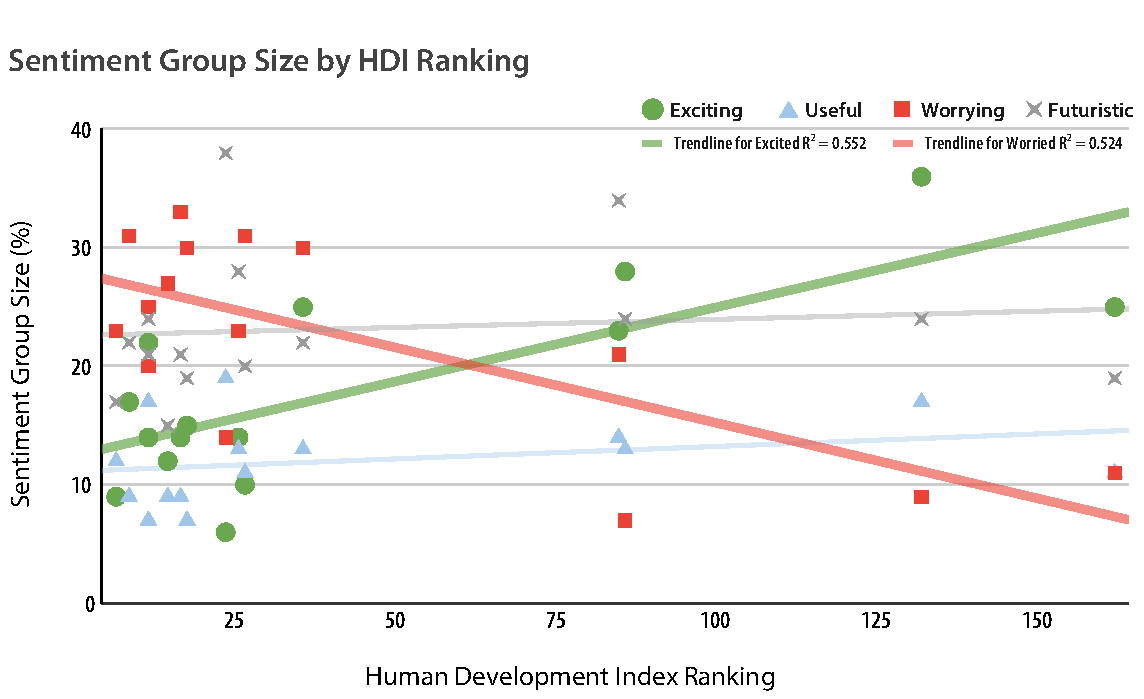
\includegraphics[width=0.7\textwidth]{figs/sentimentbyHDI.pdf}
  \vspace{-0.3cm}
  \caption{Scatter plot of weighted sentiment group size for each country, by HDI rank of the country. Trendlines shown for all four sentiment groups, with \Exciting/ at $R^2 = 0.552$ and \Worrying/ at $R^2 = 0.524$. }
  \label{fig:scatter}
\end{figure*}

Consistent with our expectation that developed countries (those most-developed, by HDI rank) would share similarities, the dominant sentiment groups in Germany, Australia, Finland, Belgium, Canada, the US, and France were \Worrying/ followed by \Futuristic/ (see Table~\ref{tab:sentimentgroups}). Spain had the same two dominant sentiments, although with \Futuristic/ followed by \Worrying/.
This resonates with claims that popular press and media narratives in Western, English-speaking regions have emphasized potential threats of AI~\cite{cave2018portrayals, fast2017long, horvitz2012interim}.

By contrast, we see respondents in developing countries tend to take a more optimistic view of AI's future effects. Respondents in China, India, and Nigeria were least likely to describe AI as \Worrying/ and more likely to describe it as \Exciting/.

Singapore, Poland, and Brazil followed a different pattern, with more balanced numbers of \Worrying/ and \Exciting/.

We can see this relationship more directly in Figure~\ref{fig:scatter} where \Exciting/ and \Worrying/ show clear trends with HDI rank. \Futuristic/ and \Useful/ however do not seem to have a relationship with HDI, highlighting that the development of a country is just one factor in how public opinion towards AI is shaped.

South Korea has a unique profile among the countries surveyed, having the largest percentage in the both the \Useful/ (19\%) and \Futuristic/ (38\%) sentiment groups. South Korean respondents also had the lowest percentage of \Exciting/ (6\% versus 9-36\% in all other countries).
These findings are consistent with South Koreans' high level of exposure to technology: South Korea boasts the world's highest robot density~\cite{ifr2018}, is one of the largest global investors in smart buildings~\cite{ducker2019}, and may be ``at the vanguard of a revolution in AI and big data healthcare''~\cite{nature2019}. Consistent with this, South Korean respondents often mentioned AI assistants and home automation, which may contextualize AI as a more familiar, everyday technology:

\begin{lq2}
\item AI is everywhere from hospitals to homes and cars.~\aff{South Korea}
\item Use big data to make daily life more convenient.~\aff{South Korea}
\item With just the smartphone, I can check the gas, temperature, and the foods in the fridge.~\aff{South Korea}
\item Self-driving car, automated production, convenient daily life~\aff{South Korea}
\end{lq2}


\section{Discussion and Outlook}
We conducted a large-scale investigation of sentiment towards AI across a range of countries. Rather than presupposing particular sentiment, we began with open-ended responses and looked for emergent themes. Our findings revealed sentiment groups as a distinguishing feature, with respondents in different countries finding AI to be \Exciting/, \Useful/, \Worrying/, and \Futuristic/ to varying degrees. These groups provide one nuanced alternative to understanding people's feelings towards AI, rather than considering their orientation to AI as simply positive or negative. While some of these themes have been seen in other literature, here we have documented them occurring unprompted in 15 countries and added richer detail about the sentiment and the mechanisms which inspire this sentiment.

The spontaneously generated open-ended responses reflect a number of key dialogues that have appeared in public discussions and the media~\cite{cave2018portrayals,chuan2019,stone2016artificial,ouchchy2020}, for example, that AI offers significant improvements for health; that AI is associated with privacy issues, job loss, and social isolation; and that AI could be either a significant boon or a significant threat to humanity. The data provide some indication of the ways in which these concepts, as well as different sources of information  (e.g. fiction, news reports, or personal experience) influence sentiment.

This suggests many fruitful avenues for further exploration. For example, it would be valuable to more formally measure and analyze the relationship between media and pop culture narratives in different countries and the presence of these sentiment groups, as well as tracing the relationship and movement of narratives across countries. Further, it would be useful to explore other factors that likely influence these sentiment groups, such as country culture and economy; institutional trust~\cite{chen2020,zhang2022}; presence, awareness, and availability of AI technologies such as customer service chatbots, personal assistants, and more; and personal, formative experiences using AI technology. It would also be worthwhile to explore how sentiment groups affect behavior such as adoption of AI technologies and public opinion on topics such as research funding and regulation.

Public opinion has the potential to shape (and be shaped by) technology development processes and decisions. For example, public opinion can affect whether the public supports research funding for AI. As another example, a negative opinion of a particular technology may discourage consumers from purchasing it. Conversely, new product offerings that rely on AI may influence the public's opinion of AI.

While public opinion can be a beneficial influence, it has also been argued that in some cases it can have suboptimal effects. For example, public misperception or unrealistic expectations of AI may lead to unfounded fears or disappointment, resulting in unwarranted rejection of technology or a lack of support for public funding~\cite{blumberg2019, cave2018portrayals}. But how might one characterize the ``legitimacy'' of public opinion, and to what extent is such characterization a meaningful endeavor? Many issues related to AI are complex questions on which even experts can disagree. And even if experts are in alignment with each other, but not with public opinion, the public may be considering perspectives or values not taken into account by experts~\cite{zhang2022}. It is therefore a complex question how best to interpret or engage with public opinion on a given issue, or whether it might be helpful to influence it. In some cases it may be beneficial to provide the public additional information, while in others it may be more beneficial for researchers and developers to shift the perspectives and values driving the development of AI.

Possible interventions might include educational efforts in areas in which the public may benefit from additional information. Beyond that, however, our findings align with calls to develop technology that supports public values. For example, many respondents were concerned about negative impacts of AI on privacy, reinforcing the value of continued emphasis on designing and developing AI with privacy in mind, concordant with discussion of privacy by design in the EU General Data Protection Regulation (GDPR).\footnote{\url{https://eugdpr.org/}} The privacy discussion continues to evolve quickly, and best practices for AI technologies continue to be actively explored in the academic, legal, and policy communities, offering many opportunities for advances in this area. Further, our findings also suggest ways in which the design and development of particular technologies may have a favorable impact on public opinion.  For example, our findings point to the value of emphasizing AI's application to healthcare in product and research investments as well as communications. As another example, future research could explore the conditions facilitating South Korea's unusually strong impression of AI as \Useful/, to gain insight into whether or how this sentiment might resonate elsewhere via communications or technological offerings.


\section*{Acknowledgments}
We thank Dan Altman, Elie Bursztein, Ed Chi, Charina Chou, Jen Gennai, Reena Jana, Jake Lucchi, Ken Rubinstein, and Kurt Thomas for valuable contributions to this work.
We also thank the cApStAn team for their important contributions to linguistic quality and the Ipsos team for their excellent work fielding the survey.

\bibliographystyle{plain}
\footnotesize
\begin{thebibliography}{10}

\bibitem{abrassart2018}
Christophe Abrassart, Yoshua Bengio, Guillaume Chicoisne, Nathalie
  de~Marcellis-Warin, Marc-Antoine Dilhac, Sebastien Gambs, Vincent Gautrais,
  Martin Gibert, Lyse Langlois, Francois Laviolette, Pascale Lehoux, Jocelyn
  Maclure, Marie Martel, Joelle Pineau, Peter Railton, Catherine Regis,
  Christine Tappolet, and Nathalie Voarino.
\newblock Montreal declaration for responsible development of artificial
  intelligence, 2018.

\bibitem{arm2017}
{ARM | Northstar}.
\newblock {AI} today, {AI} tomorrow. awareness and anticipation of {AI}: A
  global perspective, 2017.

\bibitem{barabas2018}
Chelsea Barabas, Madars Virza, Karthik Dinakar, Joichi Ito, and Jonathan
  Zittrain.
\newblock Interventions over predictions: Reframing the ethical debate for
  actuarial risk assessment.
\newblock In {\em Proceedings of the Conference on Fairness, Accountability,
  and Transparency}, pages 62--76, 2018.

\bibitem{beyer1997contextual}
Hugh Beyer and Karen Holtzblatt.
\newblock {\em Contextual Design: Defining Customer-centered Systems}.
\newblock Elsevier, 1997.

\bibitem{biemer2008weighting}
Paul~P. Biemer and Sharon~L. Christ.
\newblock Weighting survey data.
\newblock In Edith~D. de~Leeuw, Joop~J. Hox, and Don~A. Dillman, editors, {\em
  International Handbook of Survey Methodology}, pages 317--341. Lawrence
  Erlbaum Associates New York, NY, 2008.

\bibitem{blumberg2019}
{Blumberg Capital}.
\newblock Artificial intelligence in 2019: Getting past the adoption tipping
  point, 2019.

\bibitem{brynjolfsson2014second}
Erik Brynjolfsson and Andrew McAfee.
\newblock {\em The Second Machine Age: Work, Progress, and Prosperity in a Time
  of Brilliant Technologies}.
\newblock WW Norton \& Company, 2014.

\bibitem{bucher2017algorithmic}
Taina Bucher.
\newblock The algorithmic imaginary: exploring the ordinary affects of
  {F}acebook algorithms.
\newblock {\em Information, Communication \& Society}, 20(1):30--44, 2017.

\bibitem{buolamwini2018}
Joy Buolamwini and Timnit Gebru.
\newblock Gender shades: Intersectional accuracy disparities in commercial
  gender classification.
\newblock In {\em Proceedings of the Conference on Fairness, Accountability,
  and Transparency}, pages 77--91, 2018.

\bibitem{castro2019}
Daniel Castro.
\newblock The {U}.{S}. may lose the {AI} race because of an unchecked
  techno-panic.
\newblock {\em Center for Data Innovation}, March 2019.

\bibitem{cave2019}
Stephen Cave, Kate Coughlan, and Kanta Dihal.
\newblock ``{S}cary {R}obots'': Examining public responses to {AI}.
\newblock In {\em Proceedings of the 2019 AAAI/ACM Conference on AI, Ethics,
  and Society (AIES 2019)}, pages 331--337, 2019.

\bibitem{cave2018portrayals}
Stephen Cave, Claire Craig, Kanta~Sarasvati Dihal, Sarah Dillon, Jessica
  Montgomery, Beth Singler, and Lindsay Taylor.
\newblock {\em Portrayals and perceptions of {AI} and why they matter}.
\newblock The Royal Society, 2018.

\bibitem{cave2020narratives}
Stephen Cave, Kanta Dihal, and Sarah Dillon.
\newblock {\em {AI} Narratives: A History of Imaginative Thinking about
  Intelligent Machines}.
\newblock Oxford Scholarship Online, 2020.

\bibitem{cbs2016}
{CBS News}.
\newblock 60 {M}inutes/{V}anity {F}air poll: Artificial intelligence, March
  2016.

\bibitem{princetonEthics}
{Center for Information Technology Policy} and {University Center for Human
  Values}.
\newblock Princeton dialogues on {AI} and ethics case studies.
\newblock \url{https://aiethics.princeton.edu/case-studies}.

\bibitem{chancellor2019}
Stevie Chancellor, Michael~L. Birnbaum, Eric~D. Caine, Vincent M.~B. Silenzio,
  and Munmun De~Choudhury.
\newblock A taxonomy of ethical tensions in inferring mental health states from
  social media.
\newblock In {\em Proceedings of the Conference on Fairness, Accountability,
  and Transparency}, page 79–88, 2019.

\bibitem{chen2020}
Yi-Ning Chen and Chia-Ho Wen.
\newblock Impacts of attitudes toward government and corporations on public
  trust in artificial intelligence.
\newblock {\em Communication Studies}, 72(1):115--131, 2020.

\bibitem{chuan2019}
Ching-Hua Chuan, Wan-Hsiu Tsai, and Su~Cho.
\newblock Framing artificial intelligence in {A}merican newspapers.
\newblock In {\em Proceedings of the 2019 AAAI/ACM Conference on AI, Ethics,
  and Society (AIES 2019)}, pages 339--344, 2019.

\bibitem{devito2017platforms}
Michael~A. DeVito, Jeremy Birnholtz, and Jeffery~T. Hancock.
\newblock Platforms, people, and perception: Using affordances to understand
  self-presentation on social media.
\newblock In {\em Proceedings of the 2017 ACM Conference on Computer Supported
  Cooperative Work and Social Computing}, pages 740--754, 2017.

\bibitem{dietterich2015rise}
Thomas~G. Dietterich and Eric Horvitz.
\newblock Rise of concerns about {AI}: Reflections and directions.
\newblock {\em Communications of the ACM}, 58(10):38--40, 2015.

\bibitem{ducker2019}
DuckerFrontier.
\newblock Smart building trends in 2019: Part 1, April 2019.

\bibitem{dutton2018}
Tim Dutton.
\newblock An overview of national {AI} strategies.
\newblock {\em Medium}, June 2018.

\bibitem{edelman2019}
Edelman.
\newblock 2019 {E}delman {AI} survey, March 2019.

\bibitem{eslami2015always}
Motahhare Eslami, Aimee Rickman, Kristen Vaccaro, Amirhossein Aleyasen, Andy
  Vuong, Karrie Karahalios, Kevin Hamilton, and Christian Sandvig.
\newblock ``{I} always assumed that {I} wasn't really that close to [her]'':
  Reasoning about invisible algorithms in news feeds.
\newblock In {\em Proceedings of the 33rd Annual ACM Conference on Human
  Factors in Computing Systems}, pages 153--162, 2015.

\bibitem{fast2017long}
Ethan Fast and Eric Horvitz.
\newblock Long-term trends in the public perception of artificial intelligence.
\newblock In {\em Thirty-First AAAI Conference on Artificial Intelligence},
  2017.

\bibitem{fjeld2020}
Jessica Fjeld, Nele Achten, Hannah Hilligoss, Adam Nagy, and Madhulika
  Srikumar.
\newblock Principled artificial intelligence: Mapping consensus in ethical and
  rights-based approaches to principles for {AI}.
\newblock {\em Berkman Klein Center Research Publication}, 2020.

\bibitem{scuEthics}
Markkula~Center for Applied~Ethics.
\newblock Ethics in technology practice.
\newblock \url{http://www.scu.edu/ethics-in-technology-practice/}.

\bibitem{funk2020}
Cary Funk, Alec Tyson, Brian Kennedy, and Courtney Johnson.
\newblock Science and scientists held in high esteem across global publics.
\newblock {\em Pew Research Center}, September 2020.

\bibitem{garvey2019sentiment}
Colin Garvey and Chandler Maskal.
\newblock Sentiment analysis of the news media on artificial intelligence does
  not support claims of negative bias against artificial intelligence.
\newblock {\em OMICS: a Journal of Integrative Biology}, 2019.

\bibitem{hawking2014}
Stephen Hawking, Max Tegmark, and Frank Wilczek.
\newblock Transcendence looks at the implications of artificial intelligence -
  but are we taking {AI} seriously enough?
\newblock {\em The Independent}, May 2014.

\bibitem{highlevel2019}
{High-Level Expert Group on Artificial Intelligence}.
\newblock Ethics guidelines for trustworthy {AI}, 2019.

\bibitem{hinkin1998brief}
Timothy~R. Hinkin.
\newblock A brief tutorial on the development of measures for use in survey
  questionnaires.
\newblock {\em Organizational Research Methods}, 1(1):104--121, 1998.

\bibitem{holbrook2003telephone}
Allyson~L. Holbrook, Melanie~C. Green, and Jon~A. Krosnick.
\newblock Telephone versus face-to-face interviewing of national probability
  samples with long questionnaires: Comparisons of respondent satisficing and
  social desirability response bias.
\newblock {\em Public Opinion Quarterly}, 67(1):79--125, 2003.

\bibitem{horvitz2012interim}
Eric Horvitz and Bart Selman.
\newblock Interim report from the panel chairs: {AAAI} {P}residential {P}anel
  on long-term {AI} futures.
\newblock In {\em Singularity Hypotheses}, pages 301--308. Springer, 2012.

\bibitem{ethicalOS}
{Institute for the Future} and {Omidyar Network}.
\newblock Ethical {OS} {T}oolkit.
\newblock \url{https://ethicalos.org}.

\bibitem{ifr2018}
{International Federation of Robotics}.
\newblock Robot density rises globally, Feb 2018.

\bibitem{ipsos2019}
Ipsos.
\newblock Widespread concern about artificial intelligence, 2019.

\bibitem{jobin2019}
Anna Jobin, Marcello Ienca, and Effy Vayena.
\newblock The global landscape of {AI} ethics guidelines.
\newblock {\em Nature Machine Intelligence}, 1:389--399, September 2019.

\bibitem{kalyanakrishnan2018opportunities}
Shivaram Kalyanakrishnan, Rahul~Alex Panicker, Sarayu Natarajan, and Shreya
  Rao.
\newblock Opportunities and challenges for artificial intelligence in {I}ndia.
\newblock In {\em Proceedings of the 2018 AAAI/ACM Conference on AI, Ethics,
  and Society (AIES 2018)}, pages 164--170. ACM, 2018.

\bibitem{kelley2021}
Patrick~Gage Kelley, Yongwei Yang, Courtney Heldreth, Christopher Moessner,
  Aaron Sedley, Andreas Kramm, David~T. Newman, and Allison Woodruff.
\newblock Exciting, useful, worrying, futuristic: Public perception of
  artificial intelligence in 8 countries.
\newblock In {\em Proceedings of the 2021 AAAI/ACM Conference on AI, Ethics,
  and Society (AIES '21)}, page 627–637, 2021.

\bibitem{lloyds2020}
{Lloyd’s Register Foundation}.
\newblock World {R}isk {P}oll report 2019, 2020.

\bibitem{mccorduck2004machines}
Pamela McCorduck.
\newblock {\em Machines Who Think}.
\newblock A K Peters/CRC Press, 1979.

\bibitem{mcdonald2019}
Nora McDonald, Sarita Schoenebeck, and Andrea Forte.
\newblock Reliability and inter-rater reliability in qualitative research:
  Norms and guidelines for {CSCW} and {HCI} practice.
\newblock In {\em Proceedings of the 22nd ACM Conference on Computer Supported
  Cooperative Work and Social Computing (CSCW 2019)}, 2019.

\bibitem{micallef2014eulerape}
Luana Micallef and Peter Rodgers.
\newblock {eulerAPE}: drawing area-proportional 3-{V}enn diagrams using
  ellipses.
\newblock {\em PloS one}, 9(7):e101717, 2014.

\bibitem{mozilla2019}
Mozilla.
\newblock We asked people around the world how they feel about artificial
  intelligence. {H}ere's what we learned., 2019.

\bibitem{nature2019}
Nature.
\newblock {AI} and big data healthcare in {K}orea.
\newblock {\em Nature Focal Point}, March 2019.

\bibitem{neudert2020}
Lisa-Maria Neudert, Aleksi Knuutila, and Philip~N. Howard.
\newblock Global attitudes towards {AI}, machine learning \& automated decision
  making: Implications for involving artificial intelligence in public service
  and good governance.
\newblock {\em Oxford Internet Institute}, 2020.

\bibitem{nils2009}
Nils~J. Nilsson.
\newblock {\em The Quest for Artificial Intelligence: A History of Ideas and
  Achievements}.
\newblock Cambridge University Press, 2009.

\bibitem{northeastern2018}
{Northeastern University and Gallup}.
\newblock Optimism and anxiety: Views on the impact of artificial intelligence
  and higher education's response, January 2018.

\bibitem{openAI2019}
OpenAI.
\newblock Better language models and their implications.
\newblock {\em OpenAI Blog}, Feb 2019.

\bibitem{ouchchy2020}
Leila Ouchchy, Allen Coin, and Veljko Dubljevi{\'c}.
\newblock {AI} in the headlines: The portrayal of the ethical issues of
  artificial intelligence in the media.
\newblock {\em AI \& Society}, 35:927--936, 2020.

\bibitem{googleAI}
Sundar Pichai.
\newblock {AI} at {G}oogle: our principles, June 2018.
\newblock \url{http://www.blog.google/technology/ai/ai-principles/}.

\bibitem{rader2015understanding}
Emilee Rader and Rebecca Gray.
\newblock Understanding user beliefs about algorithmic curation in the
  {F}acebook news feed.
\newblock In {\em Proceedings of the 33rd Annual ACM Conference on Human
  Factors in Computing Systems}, pages 173--182, 2015.

\bibitem{raghavan2020}
Manish Raghavan, Solon Barocas, Jon Kleinberg, and Karen Levy.
\newblock Mitigating bias in algorithmic hiring: Evaluating claims and
  practices.
\newblock In {\em Proceedings of the 2020 Conference on Fairness,
  Accountability, and Transparency}, page 469–481, 2020.

\bibitem{salkind2010}
Neil~J. Salkind, editor.
\newblock {\em Encyclopedia of Research Design}, volume~1.
\newblock Sage, 2010.

\bibitem{sambasivan2019toward}
Nithya Sambasivan and Jess Holbrook.
\newblock Toward responsible {AI} for the next billion users.
\newblock {\em Interactions}, 26(1):68--71, 2019.

\bibitem{sanchez-mondero2020}
Javier S\'{a}nchez-Monedero, Lina Dencik, and Lilian Edwards.
\newblock What does it mean to `solve' the problem of discrimination in
  hiring?: Social, technical and legal perspectives from the {UK} on automated
  hiring systems.
\newblock In {\em Proceedings of the 2020 Conference on Fairness,
  Accountability, and Transparency}, page 458–468, 2020.

\bibitem{scharre2018army}
Paul Scharre.
\newblock {\em Army of None: Autonomous Weapons and the Future of War}.
\newblock WW Norton \& Company, 2018.

\bibitem{stone2016artificial}
Peter Stone, Rodney Brooks, Erik Brynjolfsson, Ryan Calo, Oren Etzioni, Greg
  Hager, Julia Hirschberg, Shivaram Kalyanakrishnan, Ece Kamar, Sarit Kraus,
  et~al.
\newblock Artificial intelligence and life in 2030.
\newblock {\em One Hundred Year Study on Artificial Intelligence: Report of the
  2015-2016 Study Panel}, page~52, 2016.

\bibitem{european2017}
{The European Commission}.
\newblock Special {E}urobarometer 460: Attitudes towards the impact of
  digitisation and automation on daily life, May 2017.

\bibitem{un2014}
{United Nations}.
\newblock World economic situation and prospects: Country classification, 2014.

\bibitem{ur2012smart}
Blase Ur, Pedro~Giovanni Leon, Lorrie~Faith Cranor, Richard Shay, and Yang
  Wang.
\newblock Smart, useful, scary, creepy: perceptions of online behavioral
  advertising.
\newblock In {\em Proceedings of the Eighth Symposium on Usable Privacy and
  Security (SOUPS) 2012}, 2012.

\bibitem{warshaw2016intuitions}
Jeffrey Warshaw, Nina Taft, and Allison Woodruff.
\newblock Intuitions, analytics, and killing ants: Inference literacy of high
  school-educated adults in the {US}.
\newblock In {\em Proceedings of the Twelfth Symposium on Usable Privacy and
  Security (SOUPS) 2016}, pages 271--285, 2016.

\bibitem{west2018}
Darrell~M. West.
\newblock Brookings survey finds divided views on artificial intelligence for
  warfare, but support rises if adversaries are developing it.
\newblock {\em Brookings}, August 2018.

\bibitem{wilson2014}
Max~L. Wilson, Ed~H. Chi, Stuart Reeves, and David Coyle.
\newblock Repli{CHI}: The {W}orkshop {II}.
\newblock In {\em CHI Extended Abstracts '14}, page 33–36, 2014.

\bibitem{you2015}
Jia You.
\newblock A 100-year study of artificial intelligence? {M}icrosoft {R}esearch's
  {E}ric {H}orvitz explains.
\newblock {\em Science}, January 2015.

\bibitem{zhang2022}
Baobao Zhang.
\newblock Public opinion toward artificial intelligence.
\newblock In Justin Bullock, Baobao Zhang, Yu-Che Chen, Johannes Himmelreich,
  Matthew Young, Antonin Korinek, and Valerie Hudson, editors, {\em Oxford
  Handbook on AI Governance}. Oxford University Press, 2022.

\bibitem{zhang2019artificial}
Baobao Zhang and Allan Dafoe.
\newblock Artificial intelligence: American attitudes and trends.
\newblock {\em Available at SSRN 3312874}, 2019.

\end{thebibliography}





\normalsize

\section*{Appendix: Select Questions}
\noindent{Note that some questions were modified from or replicate other questions in the literature or the canon of public opinion surveys}. For additional select questions used in the instrument see \href{https://arxiv.org/abs/2001.00081}{arXiv:2001.00081}

\small 

\question{Unaided Sentiment}
\sample{Ask All}
\questiontext{What feelings or emotions come to mind when you hear the phrase Artificial Intelligence (AI)?}
\openend

\question{Knowledge}
\sample{Ask All}
\questiontext{How much do you know about Artificial Intelligence (AI)?}
\begin{itemize}
  \setlength\itemsep{-0.3em}
\item{A lot}
\item{A moderate amount}
\item{A little}
\item{Heard of AI, but know nothing about it}
\item{Never heard of AI}
\end{itemize}

\question{Unaided Description}
\sample{Do NOT ask if ``Never heard of AI'' in Knowledge question}
\questiontext{In your own words, please describe Artificial Intelligence (AI).}
\openend

\question{Unaided Examples}
\sample{Do NOT ask if ``Never heard of AI'' in Knowledge question}
\questiontext{Please list some examples of how Artificial Intelligence (AI) is used today.}
\openend

\question{Uncomfortable Experience}
\sample{Do NOT ask if ``Never heard of AI'' in Knowledge question}
\questiontext{Have you ever had an experience with AI-related technology that made you feel uncomfortable?}
\begin{itemize}
  \setlength\itemsep{-0.3em}
\item{Yes}
\item{No}
\item{Not sure}
\end{itemize}

\question{Unaided Description of Uncomfortable Experience}
\sample{Ask if ``Yes'' to Uncomfortable Experience}
\questiontext{What happened, and what was the outcome? Please describe your experience with AI that made you feel uncomfortable.}
\openend

\vspace{12pt}

\end{document}

\end{article}
%
%\makeatletter
%\renewcommand{\AB@affillist}{}
%\renewcommand{\AB@authlist}{}
%\setcounter{authors}{0}
%\makeatother
%
\begin{article}
{A Human-Centered Methodology for Creating AI FactSheets}
{John Richards, David Piorkowski, Michael Hind, Stephanie Houde, Aleksandra Mojsilovi\'c, and Kush R. Varshney}
\graphicspath{{submissions/Richards_final/}}
\documentclass[11pt,dvipdfm]{article}
%\documentclass[11pt]{article} %The above line must be used for your camera-ready submission, which requires %a latex -> DVI -> PDF compilation pipeline.  As a workaround while you are writing your paper, you could %comment it out and use this line instead, which is compatible with pdflatex.
\usepackage{deauthor,times,graphicx,hyperref} 
\usepackage{enumitem}

\begin{document}
\title{A Human-Centered Methodology for Creating AI FactSheets}
\author{John Richards, David Piorkowski, Michael Hind,\\Stephanie Houde, Aleksandra Mojsilovi\'c, Kush R. Varshney\\IBM Research AI\\ajtr@us.ibm.com, djp@ibm.com, hindm@us.ibm.com,\\stephanie.houde@ibm.com, aleksand@us.ibm.com, krvarshn@us.ibm.com}

\maketitle
\begin{abstract}
As artificial intelligence (AI) models and services are used in a growing number of high-stakes areas, a consensus is forming around the need for a clearer record of how these models and services are developed to increase trust.
  Several proposals for higher quality and more consistent AI documentation have emerged to address ethical and legal concerns
  and general social impacts of such systems.
  However, there is little published work on how to create this documentation.
  %%Over the course of our own work in this area, we have developed 
  In this paper we describe
  a methodology for creating the form of AI documentation we call FactSheets.
  This paper describes the methodology and shares the insights we have gathered while creating nearly two dozen FactSheets.   
  Within each step of the methodology, we describe the issues
  to consider and the questions to explore with the relevant people in an organization who will be creating and consuming AI facts.
  This methodology may help foster the creation of transparent AI documentation.
\end{abstract}

\section{Introduction}

Recent work has outlined the need for increased transparency in artificial intelligence (AI) for data sets \cite{gebru-2021,data-statements,HollandHNJC2018,dataset-nut-label-2gen-2020}, models \cite{model-cards}, and services~\cite{factsheets-2019}. Proposals in support of ethical and trusted AI are also emerging ~\cite{EuropeanCommission2020,raji2019ml,ieee-2017}. Although the specifics differ, all are motivated by the desire to define a set of attributes that capture essential details of how an AI model or service was developed and tested to better understand technical, ethical, and regulatory concerns.

Despite this work on transparent reporting mechanisms, there is little consideration of how to create this documentation. 
Determining \emph{what information} to include and \emph{how to collect} that information is not straightforward.
To our knowledge this is the first work outlining a methodology for creating this documentation.
We believe this methodology can promote the creation of useful AI documentation.

We have proposed a mechanism for AI documentation called FactSheets~\cite{factsheets-2019}. FactSheets take a more general approach to AI transparency than previous 
proposals~\cite{gebru-2021,data-statements,HollandHNJC2018,model-cards,EuropeanCommission2020,EuropeanCommission2021}
in several ways:\\

\begin{itemize}[noitemsep,nolistsep]
    \item FactSheets are
tailored to the particular AI model or service being documented, and thus can vary in content 

\item FactSheets are tailored to the needs of their target audience or consumer, and thus can vary in content and format, even for the same model or service

\item FactSheets capture model or service facts from the entire AI lifecycle

\item FactSheets are compiled from information generated by multiple contributors as they perform their actions throughout this lifecycle, thereby increasing the accuracy of these facts
\end{itemize}
\hspace{.2cm}

FactSheets can document AI services in addition to individual models. We think this is important for three reasons:\\

\begin{itemize}[noitemsep,nolistsep]
    \item AI services are the building blocks for many AI applications.
Developers call the service API and
consume its output. An AI service can be an amalgam of many models
trained on many datasets.  The models and associated datasets are (direct
and indirect) components of an AI service, but they are not themselves the
interface to the developer.

\item An expertise gap often exists between the producer and consumer of
an AI service. The production team leverages the
creation of one or more AI models and thus will mostly contain data
scientists. The consumers of the API services tend to be developers.
When such an expertise gap exists, it becomes more crucial to communicate the attributes of the service in a consumable way.

\item Services composed of trusted models may not necessarily be trustworthy, so
it is prudent to also consider transparency and accountability of
services in addition to datasets and models. In doing so, we take a
functional perspective on the overall service and can test for
performance, safety, and security aspects that may go beyond what is relevant for a
model in isolation.
\end{itemize}
\hspace{.2cm}

Our methodology is motivated by user-centered design principles~\cite{mao2005}, where input from multiple stakeholders is collected to inform design. Although this takes more time than a single person designing the documentation, it is significantly more likely to meet the needs of FactSheet consumers \cite{madaio2020}.
This paper focuses on a specific form of AI documentation, FactSheets, but the techniques can be applied to other forms of AI (or even non-AI) documentation. Note, also, that our discussion centers on business applications of AI but the techniques can be applied to creating documentation for AI outside of this setting.

Before we describe our methodology in detail, we first highlight a few key concepts.  
Section~\ref{sec-lifecycle} describes the AI lifecycle, summarizing the relevant roles and workflow for the construction and deployment of an AI model or service.
Section~\ref{sec-FactSheets} describes the concept of a FactSheet and motivates the need for a FactSheet Template. Section~\ref{sec-methodology} presents our seven-step methodology for constructing useful FactSheets.
Section~\ref{sec-final} presents further guidance for those organizations planning to create FactSheets.
Section~\ref{sec-harm-safety} discusses how the methodology can help to address the needs of consumers with regards to the potential safety and harm of AI.
Finally, Section~\ref{sec-practice} touches on what we are finding as FactSheets are put into production use.

\section{The AI Lifecycle}
\label{sec-lifecycle}
The AI lifecycle includes a variety of roles, performed by people with different specialized skills and knowledge that collectively produce an AI model or service. Each role contributes in a unique way, using different tools. Figure~\ref{fig:lifecycle} specifies some common roles.

\begin{figure}
    \centering
    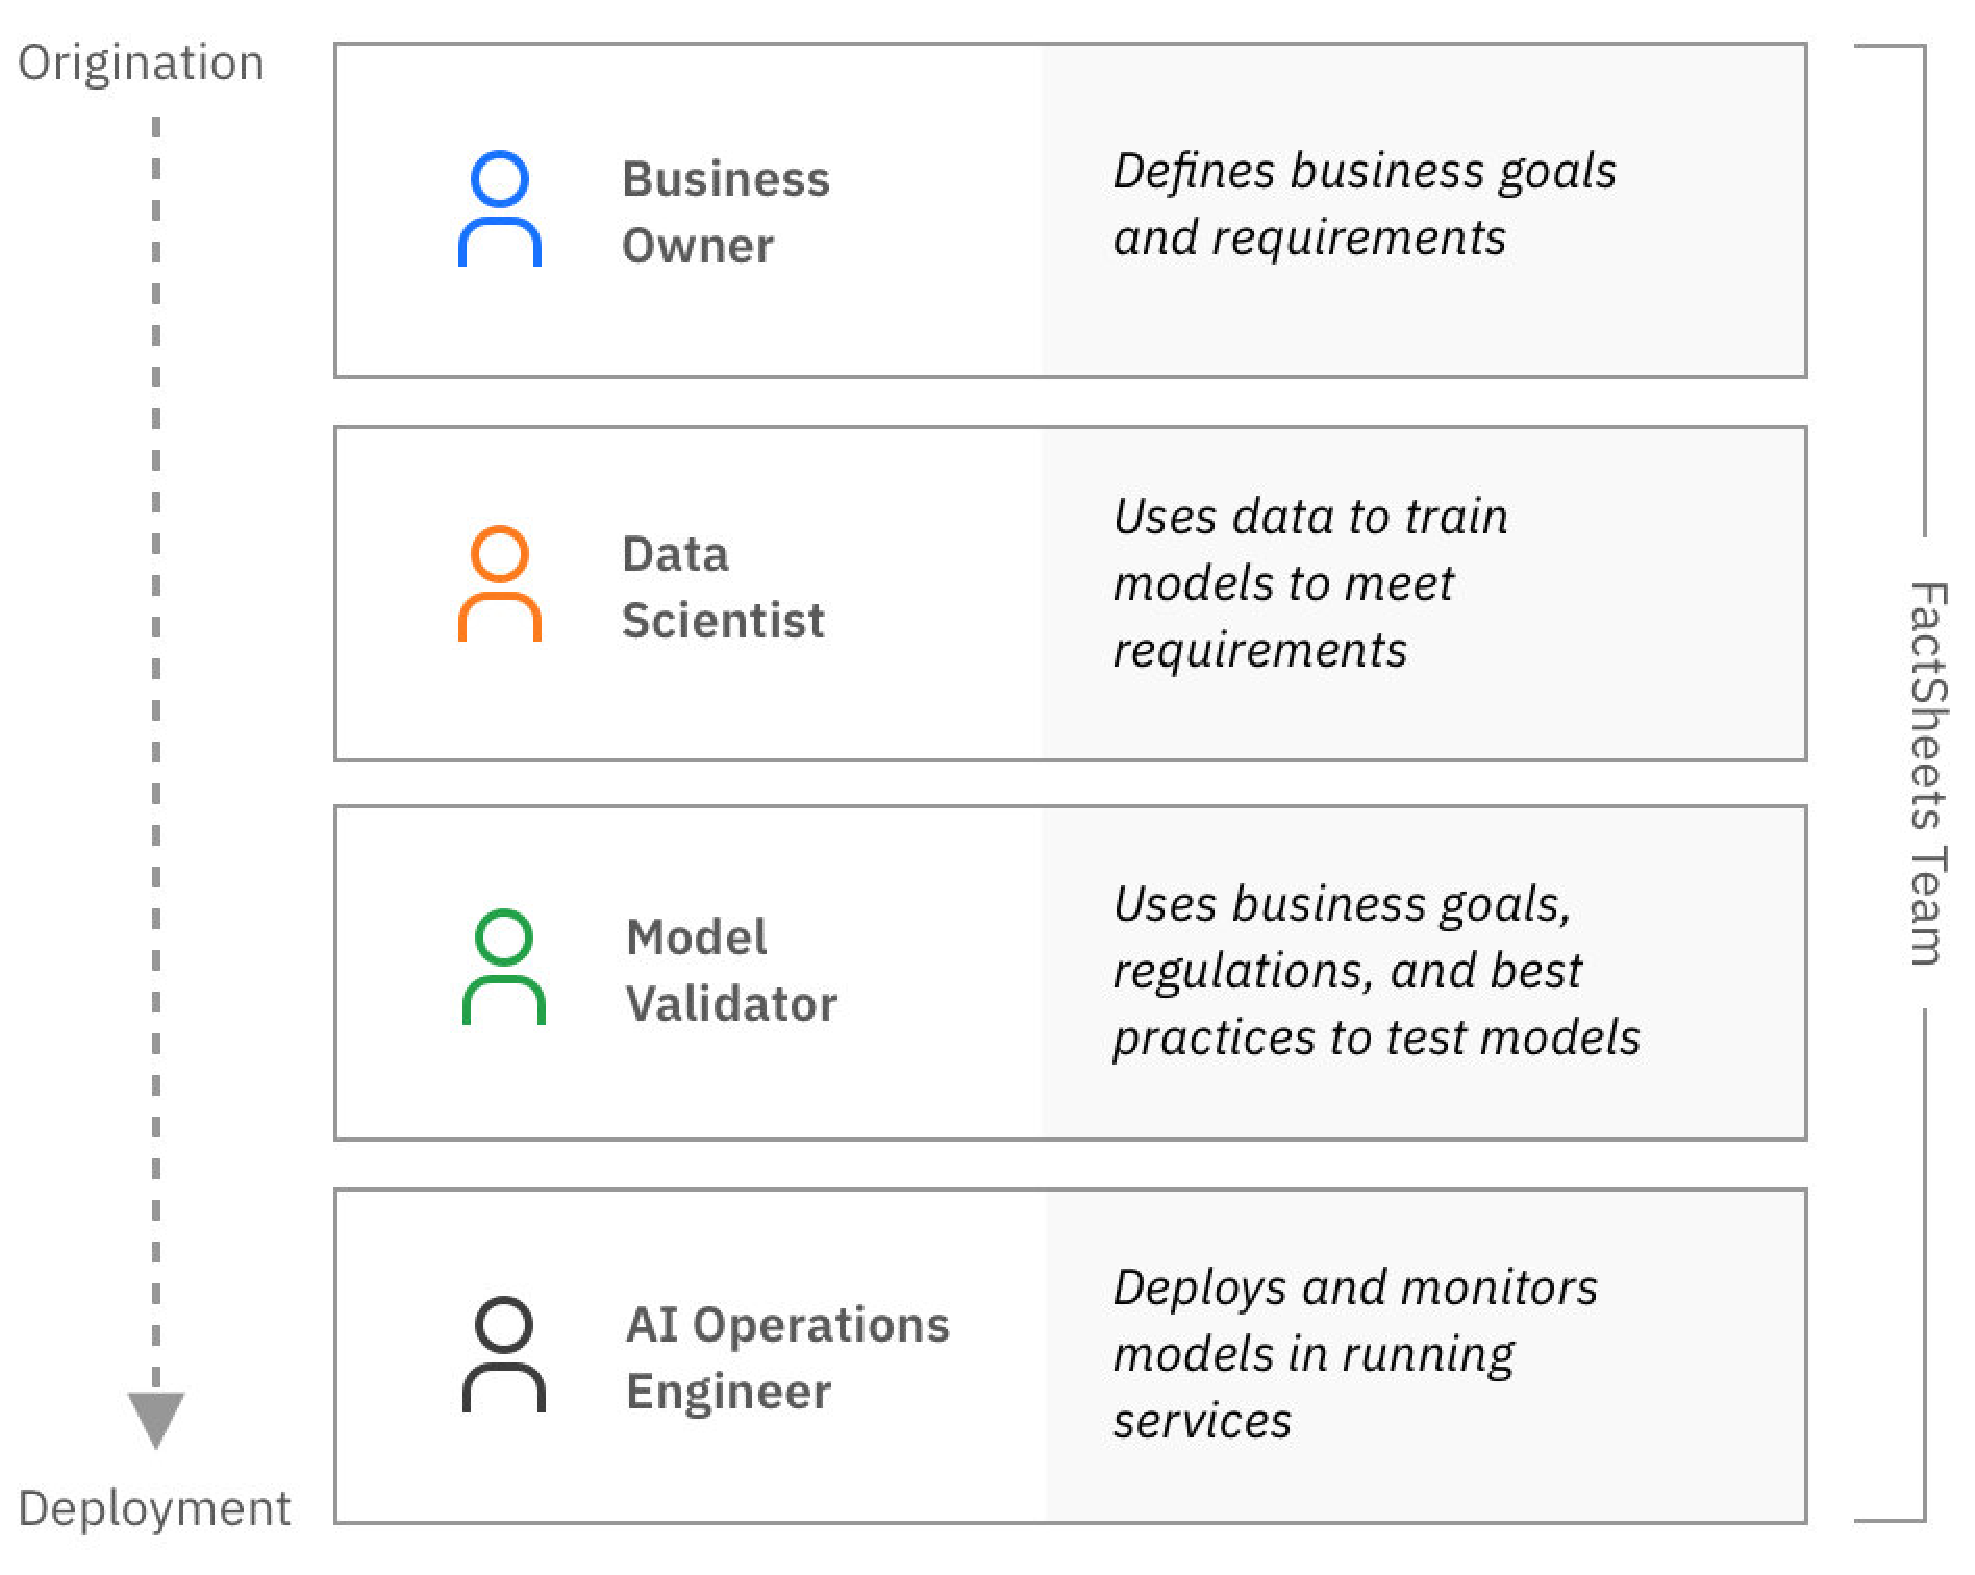
\includegraphics[width=0.45\textwidth]{figs/Img1_Roles.eps}
    \caption{Key roles in a typical AI lifecycle}
    \label{fig:lifecycle}
\end{figure}

The canonical process starts with a business owner who requests the construction of an AI model or service. The request includes the purpose of the model or service, how to measure its effectiveness, and any other constraints, such as bias thresholds, appropriate datasets, or the required levels of explainability and robustness.

The data scientist uses this information to construct a candidate model by using, most typically, a machine learning process. This iterative process includes selecting and transforming the dataset, discovering the best machine learning algorithm, tuning algorithm parameters, etc. The goal is to produce a model that best satisfies the requirements set by the business owner.

Before this model is deployed it often must be tested by an independent person, referred to as a model validator in Figure 1.
This role, often falling within the scope of model risk management~\cite{model-risk-mgmt}, 
third party testing~\cite{3rd-party-testing,eu-testing}, or certification~\cite{certification,eu-testing}, is similar to a testing role in traditional software development. 
A person in this role may apply a different test dataset to the model and independently measure metrics defined by the business owner. 
The person may also develop a "challenge" model to see if a simpler, and thus, less risky, solution could solve the same problem.
If the validator approves the model, it can be deployed.

The AI operations engineer is responsible for deploying and monitoring the model in production to ensure it operates as expected. This can include monitoring its performance metrics, as defined by the business owner. If some metrics are not meeting expectations, the operations engineer is responsible for taking actions and informing the appropriate roles.

AI lifecycles will include iteration within a role (a data scientist, building many models before passing it to a validator) or between roles (an operations engineer sending a model back to a data scientist because it is performing poorly).
More sophisticated lifecycles will likely have additional roles. A common pattern is for a model to be combined with other models or human-written code to form a service. In such a case the validator's role may be extended to also validate the full service.

A model is not a static object in the lifecycle, and thus, a FactSheet must incorporate the facts and lineage from all phases of the ``life of the model''.  This will introduce transparency not only into how the model was built and what it does, but also how it was tested, deployed, and used.

\section{FactSheets and Templates} \label{sec-FactSheets}

\textbf{FactSheets}~\cite{factsheets-2019} are a collection of information 
about how an AI model or service was developed and deployed.  
% This information includes information gathered, ideally, throughout the AI lifecycle. 
FactSheets summarize the key characteristics of a model or service for use by a variety of stakeholders. We have previously summarized the difficulties developers face when creating FactSheets~\cite{experiences-2020}. 
%%MH This paper summarizes the best practices we have discovered along the way. 
This paper describes the best practices we have developed in the process of creating FactSheets for nearly two dozen models.
These include FactSheets for standalone models as well as services that encapsulate one or more models.
%as well as multimodel ensembles or multimodel collections. 
They cover a wide range of application areas including text analysis and generation, language translation, object detection, object classification, audio signal classification, weather forecasting, agricultural crop yield prediction, and facility energy optimization.   

This work has demonstrated that although FactSheets will contain some common elements, different FactSheets will generally contain different information, at different levels of specificity, depending on domain and model type. They will also contain different information for different industries and the different regulatory schemes within which these industries operate. 

Within a particular domain or organization, FactSheets will also take on different forms, and contain different content, for different purposes. Model validators may need detailed information on data selection and cleaning, feature engineering, and accuracy and bias metrics. Business owners may need information on whether a deployed model is meeting business needs. Regulators may need a report detailing how a model complies with established practices and metrics related to safety, bias, and harm.
Thus, although there is a strong desire to create a standard template for all FactSheets, we believe this diversity illustrates that for FactSheets, \textbf{one size does not fit all}. 


We believe that standards will eventually emerge and, like nutrition labels, be useful for some purposes. 
In the foreseeable future, however, many kinds of FactSheets will be created. 
We have created the notion of \textbf{FactSheet Templates} to manage this diversity. A FactSheet Template can be thought of as specifying the categories or types of information that will be collected and displayed during and after AI development. Any given lifecycle will likely have multiple templates since different people will likely want to see different information, for different purposes, at different points in time. A large part of the job of creating FactSheets is designing the appropriate FactSheet Template(s). This is a prime focus of Section~\ref{sec-methodology}.



% -------------------------------------- FactSheet Methodology ---------------------------------------
\section{FactSheet Methodology}
\label{sec-methodology}
We now describe our seven-step methodology for the construction of useful FactSheets.
For expository purposes, the steps shown in Figure~\ref{fig:flowchart} are presented as though they flow in a single stream from beginning to end. The reality is that FactSheet production is highly iterative, especially in the early days of FactSheet adoption within an organization.

\begin{figure}
    \centering
    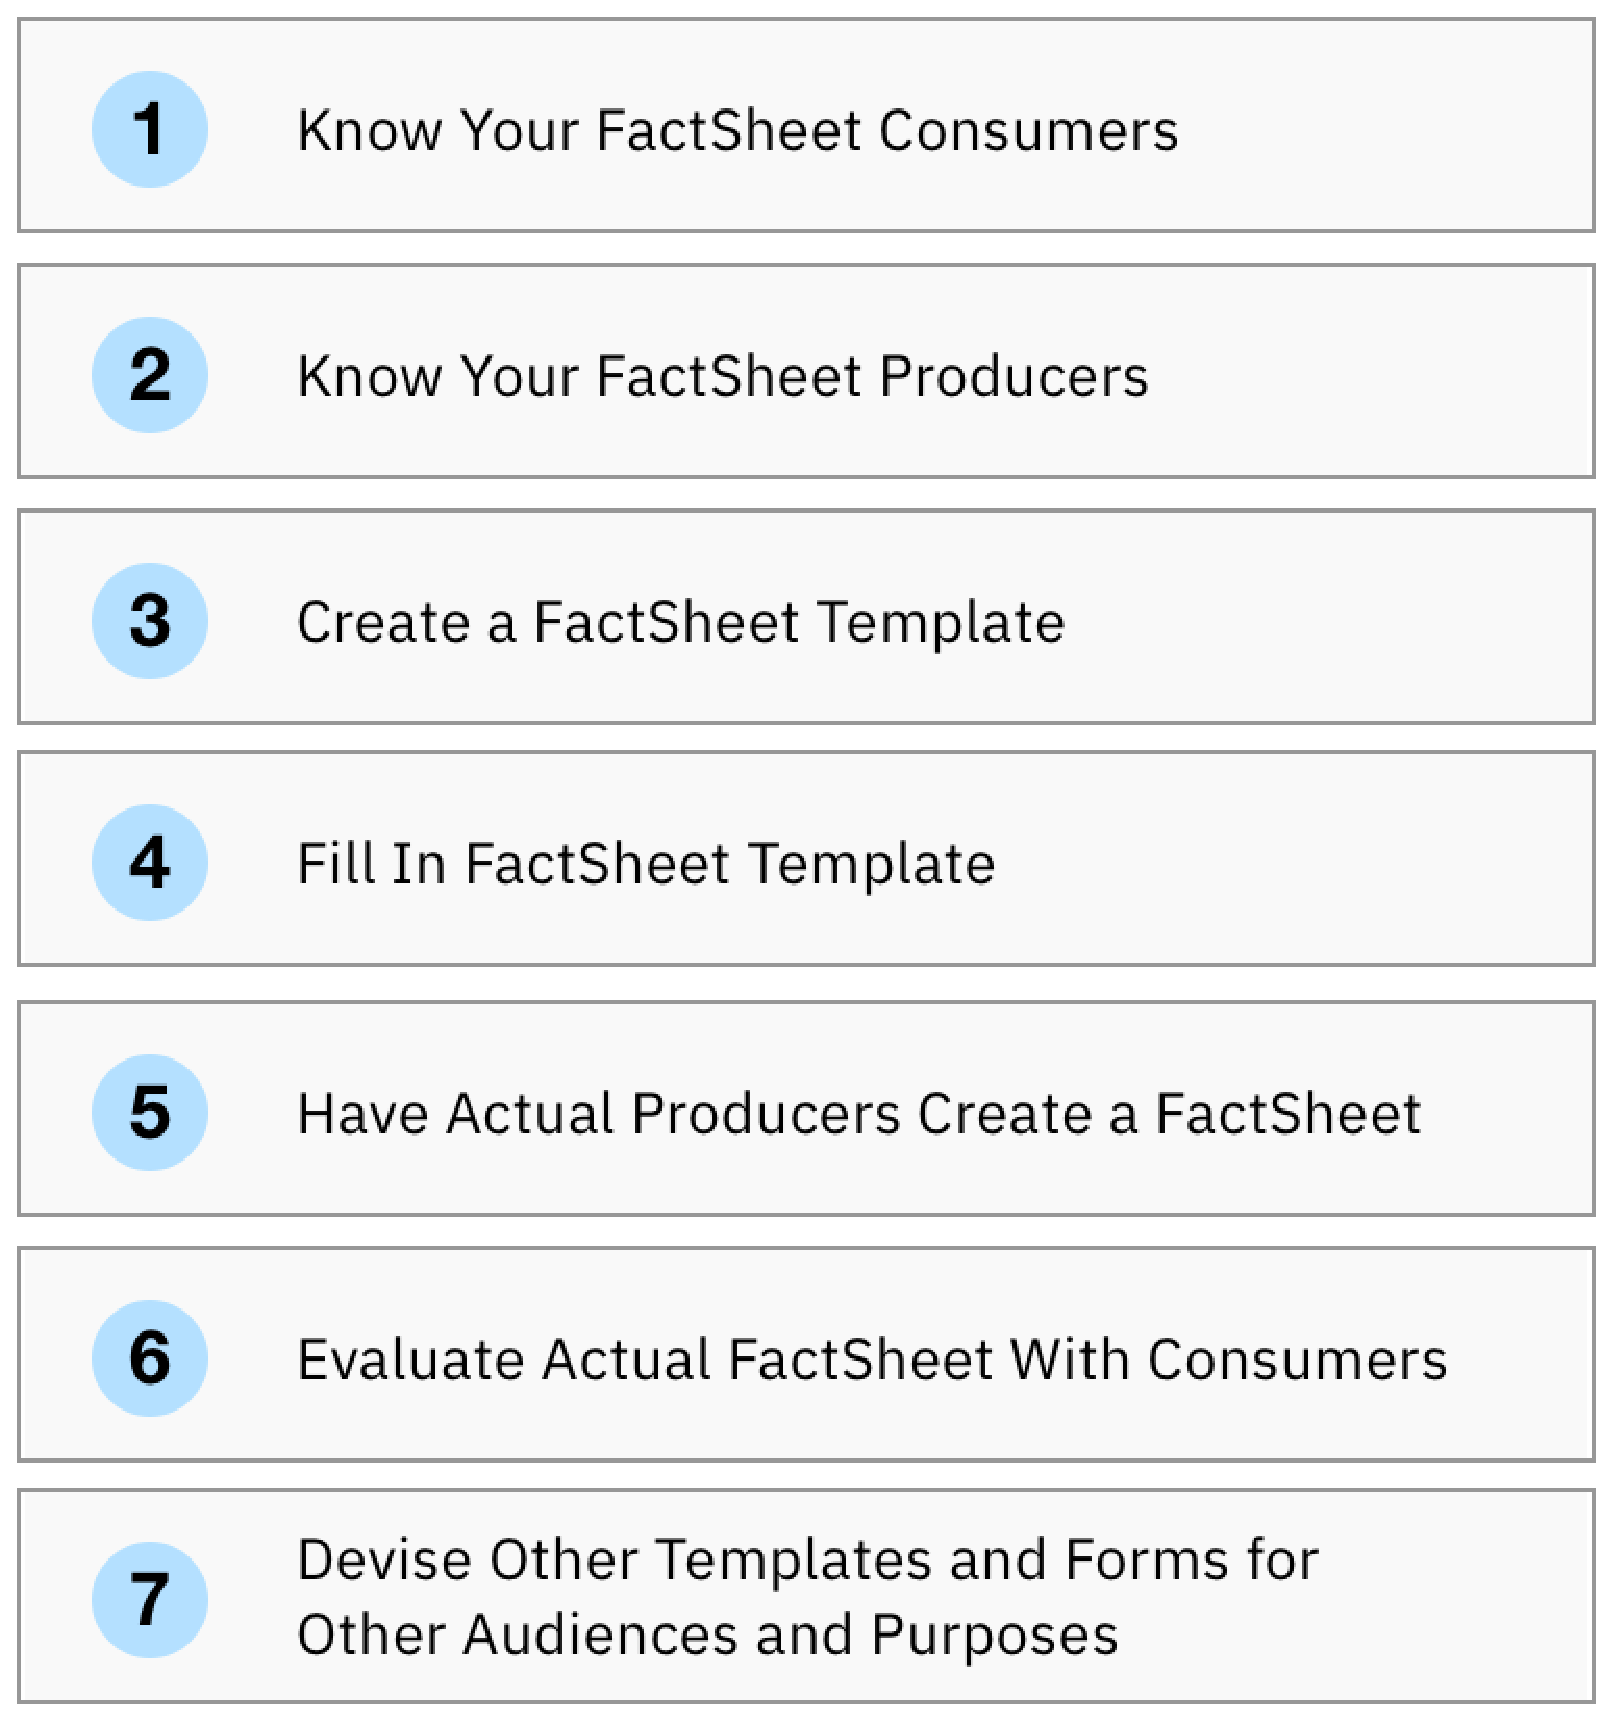
\includegraphics[width=0.45\textwidth]{figs/Img2_Steps.eps}
    \caption{Steps to produce useful FactSheets}
    \label{fig:flowchart}
\end{figure}

Each step lists the key roles involved. In addition to the more typical roles shown in Figure~\ref{fig:lifecycle}, an additional role is identified, namely the ``FactSheets Team''. This team is responsible for designing and implementing the FactSheets process within the organization. The first three steps will be driven by this team as they interview potential FactSheet consumers and producers and design the first FactSheet Template. Step 4 will largely be performed by the FactSheets Team but will benefit from the involvement of those with direct knowledge of the model or service being documented. This step may involve several iterations and informal trials with potential consumers and producers. In Step 5, FactSheet producers will generate an actual FactSheet. In Step 6, FactSheet consumers will assess the quality and usefulness of this FactSheet. The FactSheets Team will be involved in these latter steps as well but will rely heavily on others to produce and attempt to consume actual content. In Step 7, the FactSheets Team repeats the process to increase coverage and value.

To simplify the presentation in the following steps we focus on one fact producer, ``Priya'', and one fact consumer ``Carmen''. Priya is a data scientist who will generate facts about how she created her model. Carmen is a model validator who will assess the model Priya created on various dimensions including quality, simplicity, and potential risk. Of course, Priya may also be a consumer of facts produced earlier by those who assembled the training data she uses. Similarly, Carmen may be a producer of facts for those who make the final decision on deployment readiness of the model she validates.
%% mention external consumers
Although our consumer in this example, Carmen, is part of the AI lifecyle, there are other possible documentation consumers that are outside of the AI lifecycle, such as end users (e.g., a loan officer), affected users (e.g., a loan applicant), or regulators.  The same methodology would apply in these cases as well.

This may seem like a lot to think about, especially when there are multiple roles to understand and a desire to  sample multiple representative users within each role. But the important thing is to start. Find one person performing each role (some people will be performing more than one role). Spend 30 minutes in conversation with each of them. If needed, find more than one person to explore areas that are still unclear after the first conversation. To speed things up, consider bringing potential producers and consumers together in conversation at any point in this process. They may quickly converge on what information is needed and how it can be produced in a cost-effective way. 



\subsection{Step 1: Know Your FactSheet Consumers}

\begin{itemize}[noitemsep,nolistsep]
    \item Who: FactSheets Team (with potential consumers)
    \item What: Gather the information needs of potential FactSheet consumers
\end{itemize}
\hspace{.2cm}

FactSheets are produced so that they can be consumed. Understanding the information needs of FactSheet consumers is the first and most important task. Here are some of the questions to consider in this first step (with Carmen, a model validator, as the illustrative consumer):\\

\begin{enumerate}[noitemsep,nolistsep]
\item What does Carmen currently do when she performs her role?
\item What is Carmen going to be asking for when looking at a FactSheet?
\item What decisions will she be making based on the information presented?
\item How is the FactSheet going to help her do her job more effectively?
\item What are the most important pieces of information that Carmen needs to know?
\item What is Carmen's level of expertise in general data science?
\item How is Carmen's expertise going to affect the information presented?
\item Will there need to be additional definitions for terms that Carmen is unfamiliar with?
\item What is Carmen's level of expertise with respect to the model algorithms being used?
\item What explanations about the model's algorithm or results is Carmen going to need?
\item What is Carmen's level of expertise in the problem domain?
\item How is that going to affect the information presented?
\item Will Carmen need help in mapping general knowledge of the problem domain to the particular inputs, outputs, or performance indicators associated with this model?
\item Is Carmen aware of issues related to model risk, potential harm, and regulatory compliance?
\item What information is needed to assess these issues?
\end{enumerate}
\hspace{.2cm}

\subsection{Step 2: Know Your FactSheet Producers}

\begin{itemize}[noitemsep,nolistsep]
    \item Who: FactSheets Team (with potential producers)
    \item What: Gather the kinds of information FactSheet producers might generate
\end{itemize}
\hspace{.2cm}

Some facts can be automatically generated by tooling. Some facts can only be produced by a knowledgeable human. Both kinds of facts will be considered during this step. Here are some of the questions we might explore with Priya (a data scientist) about the facts she could usefully generate during the creation of a model:\\

\begin{enumerate}[noitemsep,nolistsep]
\item What facts does Priya wish she could conveniently record about the models she develops? It is often helpful to ask about the most recent model, or a model that was particularly important, or a model that was exceptionally difficult to produce, rather than discussing models in general.
\item What did Priya do during the creation of this model that is otherwise unknown to others?
\item Are there general facts about the data, the features, the model algorithm, or the training and testing Priya performs that are important to note? Why?
\item What model-specific knowledge does she have that may not be obvious to others?
\item What domain-specific knowledge does Priya have that may not be obvious to others?
\item Does Priya know who will be consuming the facts she produces? We will assume it is Carmen in this particular case. Does Priya know Carmen? Have they talked about what Carmen needs to know?
\item Is Priya aware of issues related to model risk, potential harm, and regulatory compliance?
\item What information will be needed by others to assess these issues?
\end{enumerate}
\hspace{.2cm}

\subsection{Step 3: Create a FactSheet Template}

\begin{itemize}[noitemsep,nolistsep]
    \item Who: FactSheets Team
    \item What: Define the topics and questions to be included in FactSheets
\end{itemize}
\hspace{.2cm}

What is learned in the first two steps leads directly to the most important part of creating FactSheets, namely the creation of a FactSheet Template. As discussed in Section~\ref{sec-FactSheets}, a FactSheet Template will contain questions. Each individual FactSheet will contain the answers to these questions. For example a template may start with the question ``What is this model for?''. It may then expand on that question by asking where the model is well-suited and where the model is ill-suited.

The information gathered in the first two steps will inform the creation of this FactSheet Template. You may find that details about how a model is created are much less important in your organization than information about risk assessments and regulatory compliance. Or you may find that detailed questions about robustness against adversarial attacks are needed because of the nature of the models you create or the high-stakes domains within which they are used.

Here are some of the questions to consider in creating the first iteration of a FactSheet Template. Again, this is cast in terms of Carmen's needs for information and Priya's ability to produce that information, but similar questions will apply to many of the roles in the AI lifecycle
or external consumers of the AI documentation.\\

\begin{enumerate}[noitemsep,nolistsep]
    \item What are the topics or categories of information needed?
    \item Do some of these categories have subcategories?
    \item What is a meaningful name for each category or subcategory?
    \item What kinds of information should be included in each category? For example, Carmen may want to group all the model performance metrics within a category called ``Model Performance''. Information about the representativeness of the training data might be grouped with information on the sensitivity of the model to drift in a category called, ``Potential Sources of Error''.
    \item How should each question in a category be worded so as to be both understandable and evocative for Priya? The goal here is to encourage fact producers to answer in ways that are concise, germane, and understandable.
    \item Where will the answer to a question come from? Will it be generated automatically by a tool or entered by a knowledgeable human? If the former, will Priya have some control over the frequency of fact generation or the granularity of recorded facts? If the latter, will Priya be given hints or examples of the kind of answer that would be satisfactory?
    \item Are there any regulatory, legal, or business concerns that need to be considered when answering the questions in this template?
    \item Are there different presentation formats needed for this information (for example, a short tabular summary of just key facts, or a slide format for presentations to review boards)? AI FactSheets 360~\cite{fs360} shows three different formats that might be useful.
    \item In addition to the human-readable content, is there a need for machine-readable content that Priya might generate?
\end{enumerate}

\subsection{Step 4: Fill In FactSheet Template}

\begin{itemize}[noitemsep,nolistsep]
    \item Who: FactSheets Team
    \item What: Informally assess FactSheet Template by trying to fill it in
\end{itemize}
\hspace{.2cm}

This step is where you will attempt to fill in your FactSheet Template for the first time. As you do this, informally assess the quality of the template itself. While this assessment is not a substitute for further work with Priya and Carmen (to follow), it may quickly highlight where improvements are needed. In doing this assessment, try to reflect on the template and the FactSheets it will generate from Carmen's and Priya's points of view. Ask yourself, or other members of your FactSheets Team, the following questions:\\

\begin{enumerate}[noitemsep,nolistsep]
\item Knowing what Carmen knows, will she be able to understand the information that filled-in FactSheets will include?
\item Are there details needed by Carmen that will be missing in these FactSheets?
\item Is there specialized language that Carmen will be unfamiliar with?
\item Will the information allow Carmen to make the decisions she needs to make?
\item How are these FactSheets going to help Carmen do her job more effectively?
\item What might we do to encourage Priya to answer questions in ways that provide what Carmen needs?
\end{enumerate}

\subsection{Step 5: Have Actual Producers Create a FactSheet}

\begin{itemize}[noitemsep,nolistsep]
    \item Who: Business Owner, Data Scientist, Model Validator, AI Operations Engineer (and others as defined within your organization's AI lifecycle)
    \item What: Populate a FactSheet Template with actual facts
\end{itemize}
\hspace{.2cm}

At this point you have a solid template and a good sense of how it might be used to create FactSheets. The next step is to have actual fact producers fill in the template for their part of the lifecycle. If there is a question in the template about model purpose, find someone who would actually be entering that information and have them answer the question. Ask a data scientist to answer the questions related to the development and testing of an actual model. If this model was validated, ask the model validator to enter information about that process. 
Similarly, have a person responsible for model deployment answer those questions.
If the lifecycle is not that structured, have the person responsible for most of the work create this FactSheet. 

We have found this step to be highly iterative. You can expect sections of your template to be expanded, compressed, or eliminated altogether. Individual questions will be refined within these sections. Stay alert for ideas or helpful hints about other fact producers that may surface. Follow these leads later. The goal here is to create a FactSheet that is ready for evaluation by consumers in the next step. Take the time to get this FactSheet to a level of quality and completeness that will make this next evaluation meaningful.

\subsection{Step 6: Evaluate Actual FactSheet with Consumers}

\begin{itemize}[noitemsep,nolistsep]
    \item Who: Business Owner, Data Scientist, Model Validator, AI Operations Engineer (and others as defined within your organization's AI lifecycle)
    \item What: Assess FactSheet quality with those who will be consuming FactSheets in production
\end{itemize}
\hspace{.2cm}

In this step we conduct an assessment of the quality and completeness of the actual FactSheet produced in the previous step. If the FactSheet is intended to be used by multiple roles (not uncommon), evaluate it separately for each role. To make each evaluation meaningful, ensure you have agreement with respect to the purpose of the FactSheet. Ask the consumer to imagine using this FactSheet to actually perform their work.

Each evaluation consists of two parts. The first focuses on the content in the FactSheet. The second focuses on the way in which information is presented.

\paragraph{Content Evaluation:} The goal of this part of the evaluation is to see how well the content of the FactSheet meets the specifically-designed-for information needs of the consumer. Ask your consumer to go through the FactSheet item by item with their information needs in mind and identify the following:\\

\begin{enumerate}[noitemsep,nolistsep]
    \item What information is missing?
    \item Why is that missing information important to include?
    \item How would they like this information presented?
    \item Can they give an example?
    \item What information is extraneous?
    \item Why is that information extraneous?
    \item What information is confusing or hard to understand?
    \item Why is that information hard to understand?
    \item How can that information be made more understandable?
    \item Can they give an example?
    \item Was the organization of information sensible?
    \item If not, what would they change?
\end{enumerate}
\hspace{.2cm}

Have the consumer rank the information presented in this FactSheet from most important to least important. Remember to include the information that was noted as missing in this ranking. If time permits, have them share their views about the FactSheet with your larger group. Encourage discussion and ask questions about any unexpected findings, which can often identify gaps in the underlying lifecycle process or confusion about roles. Addressing these gaps can pay large dividends.

\paragraph{Presentation Evaluation:} The goal of this part of the evaluation is to see if the way that information is \textit{presented} meets the specifically-designed-for information needs of the consumer. Since some of the information you collect may be visual, make sure to allow for that type of feedback. Ask each consumer to go through the FactSheet item by item with their information needs in mind and identify these things:\\

\begin{enumerate}[noitemsep,nolistsep]
    \item Is this information presented in an unexpected way?
    \item How can the information be presented differently?
    \item Why is this alternative a better way to present this information?
    \item Can they draw or describe an example?
    \item If the information presentation includes interactive elements, are they useful?
    \item How can they be made more useful?
    \item Why is that more useful?
    \item If they could add or change the way that information is presented, how would they?
    \item Why is this addition or change an improvement?
    \item Is this, overall, the right format for presenting this information?
    \item What format would be more suitable?
    \item Why is that format more suitable?
\end{enumerate}

\subsection{Step 7: Devise Other Templates and Forms for Other Audiences and Purposes}

\begin{itemize}[noitemsep,nolistsep]
    \item Who: FactSheets Team (and others as appropriate)
    \item What: Evolve existing templates and create new ones
\end{itemize}
\hspace{.2cm}


By now you will have created a refined FactSheet Template for use by others. They will be able to create useful and consumable FactSheets with that template. But there is more to do. There may be other consumers that need to be supported. Perhaps it is time to turn from an inward focus to an outer one, crafting templates for FactSheets to be consumed by external review boards or regulators. Or it may be time to support other stakeholders not directly involved in the AI lifecycle, such as sales personnel or the ultimate consumers of an AI service. Other formats for the same content may need to be created as well. The above steps can be followed once again. You will have  learned a surprising amount about \textit{how} to create FactSheet Templates and FactSheets from having gone through this process once. It will go faster and more smoothly now.

We encourage an ongoing process of reflecting on how well FactSheets support your AI lifecycle once they are fully incorporated and in routine use. Consider how they might be improved. Perhaps a new business opportunity in a new domain has developed or new types of models are being created that capitalize on new algorithmic research. If so, it may be time to refine existing FactSheet Templates or create new ones.

\section{Further Guidance}
\label{sec-final}

We have observed ~\cite{experiences-2020} that producers of FactSheets have a hard time imagining what consumers of FactSheets need to know and how best to provide that information. Model developers, for example, may have a sophisticated understanding of the algorithmic basis for a model, but may describe the model or its performance in ways that assume far too much knowledge on the part of a FactSheet consumer. Consumers may not really know what information they need to support their work without somewhat structured reflection. Our methodology addresses these gaps by applying a user-centered design process \cite{mao2005} to the task of creating useful AI documentation. This process need not be time consuming and expensive. Even talking with a few potential FactSheet consumers and producers will be helpful.

It should be obvious at this point that following this methodology will not lead to a single FactSheet Template across the vast array of organizations creating AI models and services. The methodology \textit{will}, however lead to FactSheets that fit the needs of a particular organization and provide real value to the corresponding AI development, deployment, and monitoring teams.

To put it a different way, one size will not fit all, at least if you dive below a short nutrition-label-like form to something that provides useful detail to all the lifecycle roles in a real organization. Even FactSheets developed with the same template will differ in interesting ways. For example, some models will have FactSheets with extensive sections on bias and fairness testing with respect to protected populations. Other models will have FactSheets for which fairness and bias considerations are truly not applicable. Within some regulated industries, FactSheets may run to a hundred or more pages whereas the FactSheet produced by a startup company providing an AI component for visual object detection may be little more than a statement of purpose, inputs, and outputs.

An extension beyond user-centered design is \emph{participatory design}, which invites not only the producers and consumers within the organizations's AI development team to contribute to the process, but also the communities affected by the deployed model or service, such as applicants or patients \cite{lee2019we,prabhakaran2020}. Moreover, by including people with lived experience of marginalization, who have an epistemic advantage in spotting potential harms, you will obtain a more comprehensive FactSheet template than if you did not have their participation \cite{fazelpour2021}.

This methodology for creating FactSheets may seem like a lot of work. Following these steps \textit{will} take more time than just having a single person write a FactSheet Template based on a limited understanding of the actions and information needs within your organization. But failing to perform these steps will incur ongoing costs in poor documentation, repeated requests between team members for missing information, insufficient testing based on faulty assumptions about data or model structure, sub-optimal business results, and exposure to unnecessary risk.

We have found that following these steps with even a small number of people, where
there is perhaps only one representative for each stage in a lifecycle, will pay dividends. We have also found that
iterating quickly, rather than spending substantial time trying to attain perfection within each iteration, will shorten the overall time needed.

\section{Harm and Safety}
\label{sec-harm-safety}
The increasing use of AI systems in high-stakes decision making has
underscored the importance of transparent reporting mechanisms. These mechanisms, including FactSheets, can lead to better understanding, and more effective mitigation of any harm or safety issues in the system, such as bias, vulnerabilities to adversarial attacks, or other undesirable societal impacts. 
For example, a section that describes a detailed analysis of bias in the training dataset can help illuminate if the system is appropriate for a particular use case.

%% One example may be a bias section that explicitly points out implicit gender bias in the data set, explains the mitigation strategy to address the bias and also presents before/after results that indicate a successful bias mitigation.

This paper describes a methodology for producing a useful transparent reporting mechanism for AI systems.  This methodology can contribute to the identification of potential harm and safety issues. The methodology does this by:
\\
\begin{itemize}[noitemsep,nolistsep]
\item Explicitly including multiple FactSheet consumers and producers in FactSheet requirements gathering (Steps 1--2) 
\item Asking questions about their concerns for harm and risk (Steps 1--2) 
\item Providing a feedback mechanism to allow further input (Step 6)
\item Including a broad range of perspectives in the development of FactSheets (Steps 1--7)
\end{itemize}
\hspace{.2cm}


This process will increase the likelihood that FactSheets will provide the information needed to understand and mitigate potential harm or safety issues with an AI system.
  
\section{In Practice}
\label{sec-practice}
% This is all coming out super vague since I don't want to mention specific counts or quotes. @John, I'll leave it to you to tell me if something needs to be expanded or cut.
We have begun evaluating the FactSheets methodology across three teams within our company and have received strong positive feedback and calls for widespread adoption for both new and existing models and services. One early benefit has become evident from the work carried out by fact producers, who were primarily data scientists. They found that the step of identifying consumers and their documentation-related use cases provided them with a perspective and a sense of purpose that was lacking in their prior documentation efforts. They described how having a persona (or sometimes a specific person) in mind enabled them to more carefully shape their documentation to meet known needs, a strategy used by data scientists more generally when communicating about their models~\cite{piorkowski2021ai}. By having specific users in mind, data scientists were able to constrain \textit{what} facts to document and \textit{how} to present them, lessening the uncertainty that they reported experiencing in the past.

The benefits of the FactSheet methodology do not come without costs. Our FactSheet creators spent up to 24 working hours crafting a complete FactSheet, with roughly half that time spent gathering feedback from consumers and iterating on content to make it more consumable. These costs can be reduced with better technology to support the creation and curation of facts. But we note that the multidisciplinary nature of AI model development, with each role having their own distinct knowledge, information needs, and preferred tools for accomplishing their work, will continue to require a focus on collaborative activities with their attendant costs and complexities (such as scheduling meetings). Bridging the gap between roles while addressing the back-and-forth, iterative nature of creating FactSheets remains a challenge to be overcome.\footnote{An earlier version of this paper~\cite{FactSheets-Methodology-arxiv-2020}
includes two illustrative FactSheet templates created using this methodology.  The templates are for the same model, but for two different consumers, illustrating the generality of the approach.}


\vspace{-.1cm}
%\bibliographystyle{ACM-Reference-Format}

%% MH: Journal requires refs to be in tex file.
%% So, I took the bbl file from overleaf and pasted it below.
%% If we make any updates to references we need to uncomment the
%% 2 lines below and remove the bib stuff below and add the new
%% bbl contents
% \bibliographystyle{abbrv}
% \bibliography{refs2}

\begin{thebibliography}{10}

\bibitem{factsheets-2019}
M.~Arnold, R.~K.~E. Bellamy, M.~Hind, S.~Houde, S.~Mehta, A.~Mojsilovi{\'c},
  R.~Nair, K.~N. Ramamurthy, A.~Olteanu, D.~Piorkowski, D.~Reimer, J.~Richards,
  J.~Tsay, and K.~R. Varshney.
\newblock {FactSheets}: Increasing trust in {AI} services through supplier’s
  declarations of conformity.
\newblock {\em IBM Journal of Research \& Development}, 63(4/5), Sept. 2019.

\bibitem{data-statements}
E.~M. Bender and B.~Friedman.
\newblock Data statements for natural language processing: Toward mitigating
  system bias and enabling better science.
\newblock {\em Transactions of the Association of Computational Linguistics},
  2018.

\bibitem{dataset-nut-label-2gen-2020}
K.~S. Chmielinski, S.~Newman, M.~Taylor, J.~Joseph, K.~Thomas, J.~Yurkofsky,
  and Y.~C. Qiu.
\newblock The dataset nutrition label (2nd gen): Leveraging context to mitigate
  harms in artificial intelligence.
\newblock In {\em NeurIPS 2020 Workshop on Dataset Curation and Security}, Dec.
  2020.

\bibitem{EuropeanCommission2021}
{European commission}.
\newblock Europe fit for the digital age: Commission proposes new rules and
  actions for excellence and trust in artificial intelligence.
\newblock Brussels, Belgium, Apr. 2021.

\bibitem{eu-testing}
{European Union}.
\newblock {CE Marking}.
\newblock
  \url{https://europa.eu/youreurope/business/product-requirements/labels-markings/ce-marking/index_en.htm#shortcut-3}.

\bibitem{fazelpour2021}
S.~Fazelpour and M.~De-Arteaga.
\newblock Diversity in sociotechnical machine learning systems.
\newblock arXiv:2107.09163, 2021.

\bibitem{gebru-2021}
T.~Gebru, J.~Morgenstern, B.~Vecchione, J.~Wortman~Vaughan, H.~Wallach,
  H.~Daum{\'e}, {III}, and K.~Crawford.
\newblock Datasheets for datasets.
\newblock {\em Communications of the ACM}, 64(12):86--92, 2021.

\bibitem{experiences-2020}
M.~Hind, S.~Houde, J.~Martino, A.~Mojsilovic, D.~Piorkowski, J.~Richards, and
  K.~R. Varshney.
\newblock Experiences with improving the transparency of {AI} models and
  services.
\newblock In {\em Extended Abstracts of the 2020 CHI Conference on Human
  Factors in Computing Systems}, CHI EA ’20, page 1–8, New York, NY, USA,
  2020. Association of Computing Machinery.

\bibitem{HollandHNJC2018}
S.~Holland, A.~Hosny, S.~Newman, J.~Joseph, and K.~Chmielinski.
\newblock The dataset nutrition label: A framework to drive higher data quality
  standards.
\newblock arXiv:1805.03677, May 2018.

\bibitem{fs360}
{IBM Research}.
\newblock {AI FactSheets 360 website}.
\newblock https://aifs360.mybluemix.net.

\bibitem{ieee-2017}
IEEE.
\newblock P7006 --- standard for personal data artificial intelligence ({AI})
  agent.
\newblock https://standards.ieee.org/project/7006.html, 2017.

\bibitem{lee2019we}
M.~K. Lee, D.~Kusbit, A.~Kahng, J.~T. Kim, X.~Yuan, A.~Chan, D.~See,
  R.~Noothigattu, S.~Lee, A.~Psomas, and A.~D. Procaccia.
\newblock {WeBuildAI}: Participatory framework for algorithmic governance.
\newblock {\em Proceedings of the ACM on Human-Computer Interaction},
  3(CSCW):181, 2019.

\bibitem{madaio2020}
M.~A. Madaio, L.~Stark, J.~Wortman~Vaughan, and H.~Wallach.
\newblock Co-designing checklists to understand organizational challenges and
  opportunities around fairness in {AI}.
\newblock In {\em Proceedings of the CHI Conference on Human Factors in
  Computing Systems}, page 318, 2020.

\bibitem{mao2005}
J.-Y. Mao, K.~Vredenburg, P.~W. Smith, and T.~Carey.
\newblock The state of user-centered design practice.
\newblock {\em Communications of the ACM}, 48(3):105--109, 2005.

\bibitem{model-cards}
M.~Mitchell, S.~Wu, A.~Zaldivar, P.~Barnes, L.~Vasserman, B.~Hutchinson,
  E.~Spitzer, I.~D. Raji, and T.~Gebru.
\newblock Model cards for model reporting.
\newblock In {\em Proceedings of the ACM Conference on Fairness,
  Accountability, and Transparency}, Atlanta, USA, Jan. 2019.

\bibitem{model-risk-mgmt}
{Office of the Comptroller of the Currency}.
\newblock
  https://www.occ.gov/news-issuances/bulletins/2011/bulletin-2011-12.html, Apr.
  2011.
\newblock OCC Bulletin 2011-12.

\bibitem{piorkowski2021ai}
D.~Piorkowski, S.~Park, A.~Y. Wang, D.~Wang, M.~Muller, and F.~Portnoy.
\newblock How {AI} developers overcome communication challenges in a
  multidisciplinary team: A case study.
\newblock {\em Proceedings of the ACM on Human-Computer Interaction},
  5(CSCW1):1--25, 2021.

\bibitem{prabhakaran2020}
V.~Prabhakaran and D.~Martin, Jr.
\newblock Participatory machine learning using community-based system dynamics.
\newblock {\em Health and Human Rights Journal}, 22(2):71--74, 2020.

\bibitem{raji2019ml}
I.~D. Raji and J.~Yang.
\newblock {ABOUT ML}: Annotation and benchmarking on understanding and
  transparency of machine learning lifecycles, 2019.

\bibitem{FactSheets-Methodology-arxiv-2020}
J.~Richards, D.~Piorkowski, M.~Hind, S.~Houde, and A.~Mojsilović.
\newblock A methodology for creating {AI FactSheets}.
\newblock https://arxiv.org/abs/2006.13796, June 2020.

\bibitem{EuropeanCommission2020}
{The European Commission's High-Level Expert Group on Artificial Intelligence}.
\newblock Ethics guidelines for trustworthy {AI}.
\newblock Brussels, Belgium, Apr. 2020.

\bibitem{certification}
{United States Consumer Product Safety Commission}.
\newblock Testing and certification.
\newblock
  \url{https://www.cpsc.gov/Business--Manufacturing/Testing-Certification}.

\bibitem{3rd-party-testing}
{United States Consumer Product Safety Commission}.
\newblock Third party testing.
\newblock
  \url{hhtps://www.cpsc.gov/Business--Manufacturing/Testing-Certification/Third-Party-Testing/}.

\end{thebibliography}


\end{document}

\end{article}
%
%\makeatletter
%\renewcommand{\AB@affillist}{}
%\renewcommand{\AB@authlist}{}
%\setcounter{authors}{0}
%\makeatother
%
\begin{article}
{Ethics, Rules of Engagement, and AI: Neural Narrative Mapping Using Large Transformer Language Models}
{Philip Feldman, Aaon Dant, David Rosenbluth}
\graphicspath{{submissions/Feldman_final/}}
\documentclass[11pt,dvipdfm]{article}
%\documentclass[11pt]{article} %The above line must be used for your camera-ready submission, which requires a latex -> DVI -> PDF compilation pipeline.  As a workaround while you are writing your paper, you could comment it out and use this line instead, which is compatible with pdflatex.
\usepackage{deauthor,times,hyperref} 
\usepackage{xcolor}
\usepackage{graphicx}
\usepackage{csquotes}
\usepackage{comment}
\usepackage{booktabs}
%\usepackage[]{geometry}
%\usepackage{listings}
%\usepackage{caption}
%\usepackage{subcaption}
%\usepackage{titlesec}
%\usepackage[titles]{tocloft}
%\usepackage{fancyhdr}
\usepackage{url}
%\usepackage{lipsum}
\usepackage{amsmath,amssymb,amsfonts}
%\usepackage{algorithmic}
%\usepackage[]{algorithm2e}
%\usepackage{paralist}

\definecolor{CMDRcolor}{HTML}{00CD00}
\definecolor{SBRDcolor}{HTML}{436EEE}

\begin{document}
\title{Ethics, Rules of Engagement, and AI: Neural Narrative Mapping Using Large Transformer Language Models}
\author{Philip~Feldman~\textit{ASRC Federal, UMBC}
        Aaron~Dant~\textit{ASRC Federal}, David Rosenbluth ~\textit{Lockheed-Martin}}% <-this % stops a space


\maketitle
\begin{abstract}
The problem of determining if a military unit has correctly understood an order and is properly executing on it is one that has bedeviled military planners throughout history. The advent of advanced language models such as OpenAI's GPT-series offers new possibilities for addressing this problem. This paper presents a mechanism to harness the narrative output of large language models and produce diagrams or \enquote{maps} of the relationships that are latent in the weights of such models as the GPT-3. The resulting \enquote{Neural Narrative Maps} (NNMs), are intended to provide insight into the organization of information, opinion, and belief in the model, which in turn  provide means to understand intent and response in the context of physical distance. This paper discusses the problem of mapping information spaces in general, and then presents a concrete implementation of this concept in the context of OpenAI's GPT-3 language model for determining if a subordinate is following a commander's intent in a high-risk situation. The subordinate's locations within the NNM allow a novel capability to evaluate the intent of the subordinate with respect to the commander. We show that is is possible not only to determine if they are nearby in narrative space, but also how they are oriented, and what \enquote{trajectory} they are on. Our results show that our method is able to produce high-quality maps, and demonstrate new ways of evaluating intent more generally.
\end{abstract}

\section{Introduction}
\label{sec:introduction}

\begin{figure}[!h]
	\centering
	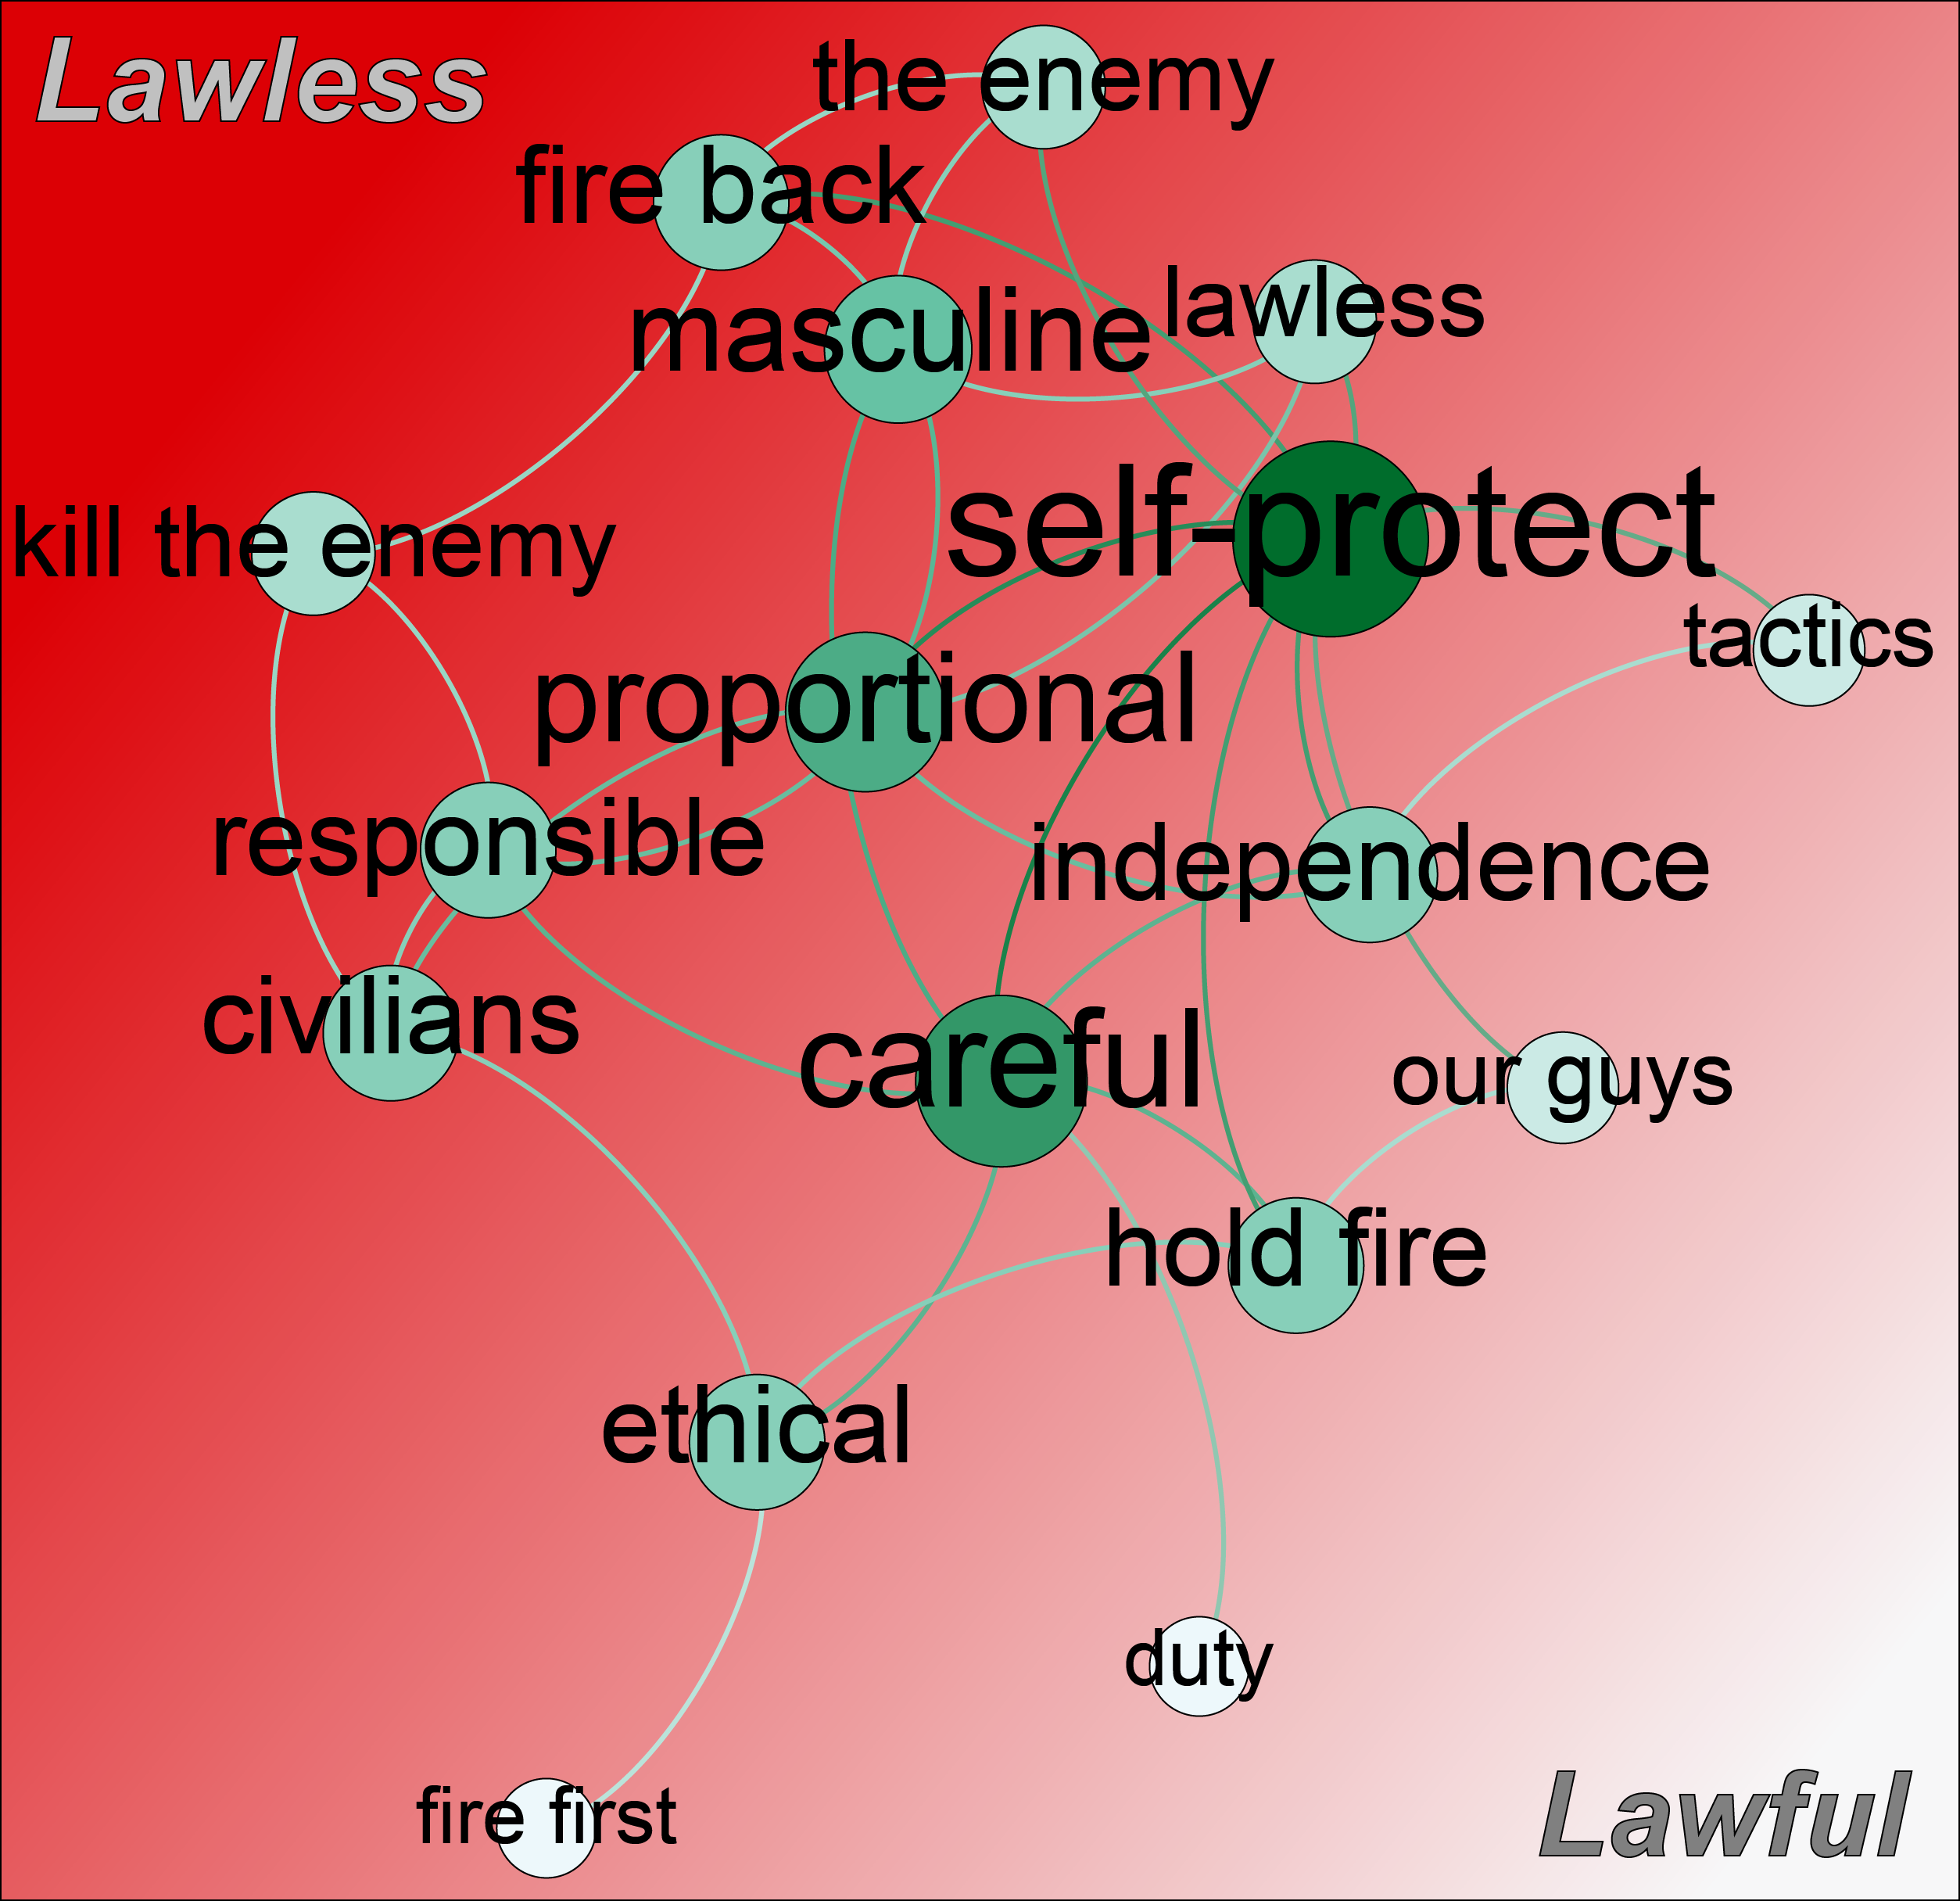
\includegraphics[height = 20em]{figs/orders_final}
	\caption{\label{fig:example}Neural Narrative Mapping Example}
\end{figure}

In the 1979 motion picture \textit{Apocalypse Now}, Captain Willard (played by Martin Sheen) is sent on a mission to assassinate Colonel Kurtz (played by Marlon Brando), a highly decorated officer who, in the words of the general authorizing the mission, has gone from \enquote{one of the most outstanding officers this country has ever produced} to someone \enquote{out there operating without any decent restraint, totally beyond the pale of any acceptable human conduct.} 

The movie explores the paradoxes in war, where some illegal acts are embraced by the command structure, some tolerated, and some are to be terminated, \enquote{with extreme prejudice.} Willard has to navigate these conflicts as he moves towards Kurtz' compound deep in Cambodia.  

\textit{Apocalypse Now} provides an example of the difficulty that any intent-aware system must face in a military context~\cite{shattuck2000communication}. Not only does the system need to determine if an order is being followed, it should also determine if the order itself is valid, so that the warriors implementing the order are not placed in ethical dilemmas. This is the goal that we attempt to address in this paper, with the concept of \textit{Neural Narrative Mapping} (NNM). By placing narrative elements at coordinates in a virtual space, we can determine sophisticated relationships between concepts that go well beyond textual comparison.

An example of this concept, described in detail later in the this paper is shown in Figure~\ref{fig:example}. This map was constructed  from narrative sequences developed by the GPT-3 Neural language model~\cite{radford2018improving} with respect to \textit{rules of engagement}. Clustering these texts produces a set of relationships. Central to this example are the concepts of self-protection and care, but there are also relationships with respect to things like ethics and masculinity. By allowing the system to develop relationships between multiple narratives, we can determine the space of possible behaviors of the soldiers such as those in \textit{Apocalypse Now} as they encountered lawful and lawless conditions.

In this paper, we will discuss mapping the relationships of such responses and how they could apply to military scenarios.  We will first introduce some background material on how to represent narratives and relationships between them. Secondly, we will show how we can incorporate our mapping method into a decision-making system and demonstrate it on a military scenario.



\section{Background}
Published research into determining intent generally is quite sparse with respect to determining how subordinate behavior reflects the intent of orders from a superior. Typically, the military relies on legal mechanisms and training to ensure that 1) subordinates follow the orders of their superiors, 2) That superiors issue lawful orders, and 3) that subordinates refuse to obey unlawful orders~\cite{hoff2001obeying}. This framework has existed as precedent since the Nuremberg Trials, when Nazi officers were convicted of war crimes that they had been ordered to commit~\cite{taylor2012anatomy}. These rules were codified in the Geneva Conventions of 1949 and embodied in the Army Field Manual prohibitions against issuing and obeying unlawful orders~\cite{Army_field_manual_1956}.

However, research has shown that subordinates misunderstand the intent of their superiors 50\% - 60\% of the time~\cite{shattuck2000communication}. This means that approaches such as training and legal enforcement are not effective in ensuring that the intent of a legal order is followed by a subordinate. The process of determining intent is made even more difficult by situations where communications are degraded. For example, if a superior's orders can't be understood, then it is impossible to determine whether the subordinate misunderstood the orders or whether they refused to follow them.

As a partial solution to this problem, the military will often do simulations or war games where miscommunication issues can be uncovered and corrected before they occur. Recently, work has been done in automating this process so that the space of possibilities can be explored more thoroughly~\cite{shattuck2000communication}. Such \textit{computational military tactical planning}, and has largely employed genetic algorithms to explore potential outcomes, including co-evolving friendly/enemy tactics~\cite{kewley2002computational}. 

More recently, the development of human-robot teams has required the development of more explicit forms of communicating and verifying intent. In the case of these hybrid teams \enquote{each autonomous system in the team must be able to determine their own individual tactical behaviors based upon inferences made about the human supervisor’s intent, rather than by direct response to specific command inputs.} Work by Evans, et al. Has focused on the development of shared mental models and implicit coordination based on verbal and non-verbal communication~\cite{evans2017future}.

Transformer language models (TLMs) open up new possibilities for examining intent in the context of synthetic narratives.  TLMs are trained on massive text datasets, comprising a significant fraction of the high-quality text available on the internet~\cite{brown2020language}. They implement attention-based deep neural network architectures to allow the model to selectively focus on the segments of the input text that are most useful in predicting adjacent and word tokens. Models are not trained using any hand-crafted language rules and learn to generate natural language purely by observing text data. In doing so, they capture semantic, syntactic, discourse, and even pragmatic regularities in language. A GPT model can be used for generating texts as a function of the model and a sequence of words, or \enquote{prompt}, provided by users which is specifically designed to set up the context for GPT to generate text. GPT models have been shown to generate text outputs often indistinguishable from that of humans~\cite{floridi2020gpt}. 

The transformer's ability to integrate across large amounts of data can better support the information-seeking user when using interactive systems like chatbots~\cite{yang2020iart}. Transformers open up novel avenues of research into intent that have not been available before, particularly in understanding and exploiting the ways that information is stored in and retrieved from these models.

Since the introduction of the transformer model in 2017, TLMs have become a field of study in themselves. Among them, BERT~\cite{devlin2018bert} and GPT~\cite{radford2018improving} are two of the most well known TLMs used widely in boosting the performance of diverse NLP applications. Transformers are unlike perceptrons and convolutional neural networks in that they use self attention, where the model computes its own representation of its input and output~\cite{vaswani2017attention}. Most recent research has been in increasing the performance of these models, particularly as these systems scale into the billions of parameters~\cite{radford2019language}. 

Understanding how and what kind of knowledge is stored in all those parameters is becoming a sub-field in the study of TLMs. Language models require no human supervision to train, do not have schemas like traditional databases, and can be queried using natural language. These properties make them an attractive mechanism for storing and retrieving information. Examples of information retrieval include TLMs successfully completing \enquote{cloze statements}, where the model fills in a blank~\cite{petroni2019language}, factual relationships extracted from the Wikipedia~\cite{elsahar2018t}, and general knowledge~\cite{speer2018conceptnet}. These studies showed that TLMs are often \enquote{competitive with non-neural and supervised alternatives.}~\cite{petroni2019language}

The prompt that is used to elicit specific information from these models has also become a field of study in its own right. For example,  mining-based and paraphrasing approaches can increase effectiveness in masked BERT prompts over manually created prompts~\cite{jiang2020can}. These studies demonstrated that effective prompts can be produced by  mining phrases in the Wikipedia corpus which can be generalized as template questions such as \textit{x was born in y} and \textit{capital of x is y}. These can then be filled in using sets of subject-object pairs. Improvements over manually-developed prompts using this technique can be substantial, with improvements of 60\% over manual prompts. Paraphrasing, or the simplification of a prompt using techniques such as back-translation can enhance query results further~\cite{jiang2020can}. 

Our own research has been focused on understanding how TLMs incorporate domain-specific knowledge. We fine-tuned GPT-2 models on descriptions of chess games showed that models trained on a corpora of approximately 23,000 chess games accurately replicated human gameplay patterns~\cite{feldman2020navigating}. Statistical analysis comparing the spectral characteristics of human (ground truth) and synthesized games were found to be statistically similar with a $> 97\%$ probability. This work was extended to perform sociological research on different political groups on Twitter by training GPT-2 models on the tweets of right-wing, majority, and science-focused tweets during the first year of the COVID-19 pandemic~\cite{feldman2021analyzing}. 

Using TLMs to evaluate social data is still nascent. A study by \cite{palakodety122020mining} used BERT fine tuned on YouTube comments to gain insight into community perception of the 2019 Indian election. They created weekly corpora of comments and constructed a tracking poll based on the prompts \enquote{Vote for MASK} and \enquote{MASK will win} and then compared the probabilities for the tokens for the parties BJP/CONGRESS and candidates MODI/RAHUL. The results substantially matched traditional polling.

A characteristic of TLMs is that when provided with the correct prompt, they will produce relevant content regardless of the ethical implications of the generated text.   OpenAI has shown that the GPT-3 can be \enquote{primed} using \enquote{few-shot learning}~\cite{brown2020language}. Using this technique, McGuffie primed the GPT-3 using mass-shooter manifestos, which generated text that maintains the amoral, dangerous context of these texts~\cite{mcguffie2020radicalization}. This will become particularly important in this research, as we are particularly interested in unethical behavior in response to lawful orders.


\section{Narrative Generation using TLMs}
Narratives are defined as \enquote{a written account of connected events; or a story}. These stories are linear constructs, and are naturally suited to the presentation of a singular point-of-view over time. Narratives can range from fictional stories to detailed travelogues. 

Less known is that narratives have been used as the basis of navigation for millennia. Before the 16th century, ship's pilots collected \enquote{navigation stories} into a \textit{rutter} or \textit{pilot book}, that described coastal and open ocean routes in narrative form. Because it is difficult to have explicit spatial relationships between stories, rutters \enquote{exhibit an understanding of physical space as delimited rather than panoramic}~\cite{goldie2015early}. To obtain this \textit{panoramic} view, one needs the broader perspective provided by maps. 

Even if there were no such things as \textit{objective}, surveyed maps, it is possible to build panoramic maps based on a careful synthesis of a large set of personal, subjective descriptions. These narrative \enquote{threads} can be knitted together into a tapestry that portrays the spatial relationships, based on this collection of individual, seemingly unrelated paths. Though these maps do not have the representational rigor that objective maps have, maps based on such \textit{subjective} data still support navigation between the physical places of the world.

The same sorts of maps can be created utilizing narratives about non-physical domains. For example, narratives about philosophy can be combined to produce spatial representations such as those shown in Figure~\ref{fig:gpt3_philosophy}. More importantly for our purposes, the same technique  can be used to navigate \textit{information spaces} such as those related to military orders as in the map of Figure~\ref{fig:example}.

A large number of narratives would be needed to define the space through their overlapping tales to generate these maps. Fortunately, TLMs such as the GPT allow the generation of these narratives dynamically and with no limit. The GPT model generates narrative text by starting with a sequence of word tokens, or prompt, provided by the user. A single word token can be thought of as a query into the model. The GPT model then begins to generate text by choosing a set of words that are more likely to follow the prompt which are added to the text. It then considers the words that are most likely to come after the updated text, and repeats the process until it has generated as many tokens as the user desires. 

For example, if the model is prompted with the word \enquote{cat}, it considers that word to be the initial query. If it has learned to associate cats with fish, then it may generate the sentence \enquote{A cat likes to eat fish}. Similarly, if the model is provided with the word \enquote{wombat}, it will consider that word to be a query, and could generate the sentence \enquote{A wombat is a kind of marsupial}.This process can be extended to have the model evaluate terms that it has never seen before, through the use of a technique called \textit{prompt tuning}. 

When presented with the prompt \enquote{\textit{A floober is a flightless bird that inhabits the barren wastes of Antarctica. Like its cousin the Chinstrap Penguin, the}}, the GPT-3 produces the following output about this fictional animal:

\begin{displayquote}
\textit{\textbf{A floober is a flightless bird that inhabits the barren wastes of Antarctica. Like its cousin the Chinstrap Penguin, the} floober is a ground-dwelling bird that uses its wings primarily for mating displays. The floober's flightlessness is believed to be an adaptation to the extreme cold of Antarctica, which would make flight inefficient and possibly hazardous. It is believed that floobers lost their ability to fly because of an evolutionary tradeoff between wing size and body size, resulting in the floober having very small wings, but a large body.}
\end{displayquote}

In this generated response, we can see one of the truly novel capabilities of these large language models -- the ability to articulate internally consistent narratives  based on a starting point and orientation. Here, the starting point is a fictional penguin-like bird, and the orientation is the descriptive language that leads the model to continue the description based on the starting conditions. 

The same prompt can be used again and again to produce a statistical distribution of what this imaginary bird might be. This allows us to \enquote{map out} the expectation of what such an animal might be, based on all the items that the GPT-3 has read as part of its training set.

The GPT creates sequences of words that mimic the patterns of human production. In other words, there is a sense of the causal relationships inherent in the information stored in the model. For example, when prompted with \enquote{\textit{Smoking cigarettes causes}}, the GPT consistently responds with \enquote{\textit{cancer, heart disease, lung disease}} among other related conditions. This is not an understanding of causality per se, rather it is a reflection of the sequencing of tokens that the GPT is trained and evaluated on. These sequences naturally reflect our stated understandings including subjective bias. As such, a \textit{sequence} of statements has a particular trajectory over the \enquote{terrain} of the model. When the GPT writes a sentence, it is more like a ball rolling down a lumpy hill rather than intelligence as we perceive it as humans. 

Recursively iterating over multiple prompts that are created by the GPT in response to one or more \enquote{seed prompts} results in a sort of quasi-causal \textit{bootstrap conversation} that the model has with itself. This process provides the dynamically produced limitless content that we need to generate maps.

\section{Methods}
\label{sec:methods}
This section describes the development of the technique used to produce maps using data from the GPT-3. This work had two phases. The first was a basic proof of concept, where output from the GPT could be parsed and placed into graphs based on existing ground truth that the output could be validated against (Section~\ref{sec:initial_gpt_maps}). The second phase describes the development of an interactive map creation tool that incorporates human interaction (Section~\ref{sec:interactive_builder}). This process allows the development of maps that incorporate more subjective human understandings that are harder to validate against external datasets, such as the exploration of the ethical spaces around legal and emergent military \enquote{Rules of Engagement} (ROE).

\subsection{Initial GPT-3 Maps}
\label{sec:initial_gpt_maps}

OpenAI has developed an online \enquote{playground} for developers to test out prompts. When presented with: \enquote{\textit{Here's a short list of countries that share a border with Italy:}}

The GPT-3 continues the statement with the following text: \textit{France, Switzerland, Austria, Slovenia,	San Marino, Vatican City}.

In this example, the response is remarkably accurate. Not only are adjacent countries like France, Switzerland and Austria included, but also countries that are contained within Italy (i.e. San Marino and Vatican City).

Repeated responses vary, but they are consistent enough to produce map-like representations. For example, Figure~\ref{fig:gpt3_central_america} shows a map of Central America using the same technique. Although there are no explicit positioning instructions in the responses of the GPT, the result compares well to a geographic map, shown in Figure~\ref{fig:central_america}:

\begin{figure}[!htbp]
	\centering
	\begin{minipage}{0.45\textwidth}
		\centering
		\fbox{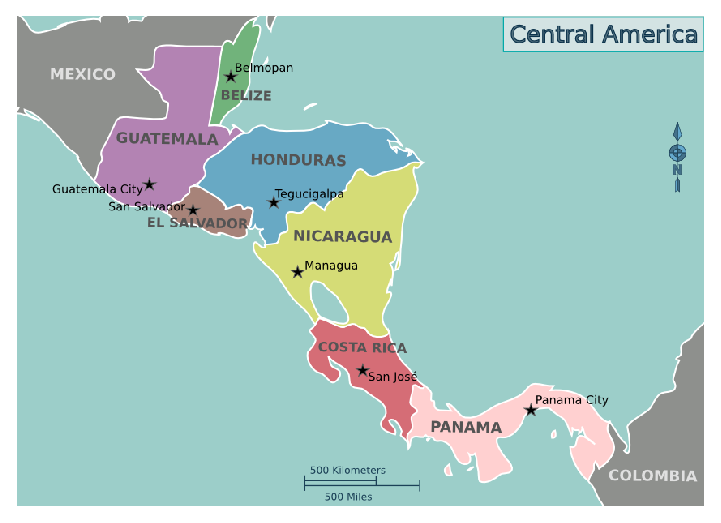
\includegraphics[height=13em]{figs/Map_of_Central_America}}
		\caption{\label{fig:central_america}Central America}
	\end{minipage}%
	\begin{minipage}{0.45\textwidth}
		\centering
		\fbox{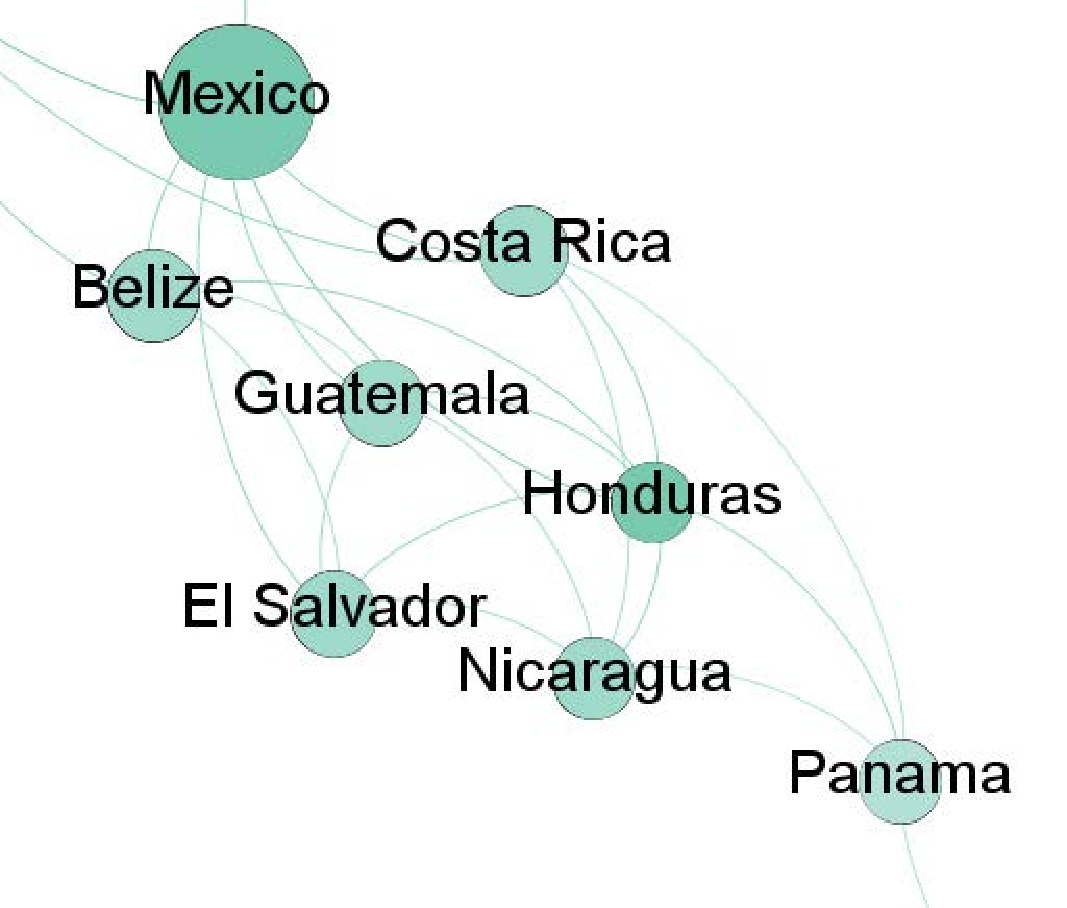
\includegraphics[height = 13em]{figs/central_america}}
		\caption{\label{fig:gpt3_central_america}Reconstruction}
	\end{minipage}%
\end{figure}

The diagram of Figure~\ref{fig:gpt3_central_america} was produced by repeatedly querying the GPT-3 with a prompt that incorporates the results of the previous prompt. This is the core of the iterative process used to generate NNM maps and is shown in detail in Algorithm~\ref{alg:map_core}. 

\begin{algorithm}
    \small
	Set $max\_queries$ to the number of queries desired \\
	Set $query\_count$ = 0 \\
	Create empty list nodes $L_{nodes}$\\
	Create an empty list of used seeds $L_{queried}$\\
	Populate initial seed list $L_{seed}$\\
	Set the prompt template $T$\\
	Set current node $N_{cur} = seed$\\
	\While{$query\_count < max\_queries$}{
		Append $N_{cur}$ to $L_{nodes}$\\
		Set query $Q$ to the $T + L_{seed}[0]$\\
		Move $seed$ from $L_{seed}$ to $L_{queried}$ \\
		$response\_text = GPT\_fn(Q)$ \\
		$L_{responses} = Parse\_fn(response\_tex)$ \\
		\ForEach{$response$ in $response\_list$}{
			\If{$ValidResponse\_fn(response)$}{
				\ForEach{$N$ in $L_{nodes}$}{
					\If{$N.name == response$}{
						$Connect\_fn(N, N_{cur})$\\
					}
				}
				\If{$response$ not in $L_{queried}$ and $response$ not in $L_{seed}$}{
						Append response to $L_{seed}$\\
						Create new node $N_{response}$\\
						Append $N_{response}$ to $L_{nodes}$\\
						$Connect\_fn(N_{response}, N_{cur})$\\
				}
			}
		}
		$query\_count += 1$
	}
	\vspace{0.5em}
	\caption{Iterative mapping algorithm}
	\label{alg:map_core}
\end{algorithm}

In Algorithm~\ref{alg:map_core}, a text \enquote{prompt template} is created that supports the incorporation of seed fragments. In Python, the template used to produce the map in Figure~\ref{fig:gpt3_central_america} was \texttt{'A short list of countries that are nearest to "\string{\string}", separated by commas:'.format($seed$)}. This allows the prompt to run repeatedly as new results are incorporated into $L_{seed}$. The graph is built out by connecting node with the value of the current $seed$ to nodes whose label matches a value in the $response\_list$. If there is no node for a $response$, one is created and connected to the current node $N_{cur}$. This process repeats until $query\_count == max\_queries$.

All the maps in this section can be validated by some kind of \enquote{ground truth,} or data that exists independently in another source. In Figures~\ref{fig:gpt3_central_america} and \ref{fig:gpt3_philosophy}, $response$ values were validated by using the Wikipedia API\cite{wiki:Wikimedia_REST_API} to check if there was an entry for each GPT response. Responses that do not have a Wikipedia entry get caught before they are added to the map. A further benefit of such ground truth is that it is possible to adjust the size of the node based on, as in this case, the number of queries against a particular topic. We can see in the maps that \enquote{Mexico} and \enquote{Stoicism} get more searches than the other items in the map.

The graphs created using this process were then used to create a GML (Graph Modeling Language) file that can be read by a variety of graphing libraries and packages. The maps shown here were produced using Gephi\footnote{gephi.org}, using the ForceAtlas layout~\cite{jacomy2014forceatlas2}. 

This approach need not be limited to geography. Figure~\ref{fig:gpt3_philosophy} shows a map created using the prompt \textit{\enquote{\rule{0.5cm}{0.15mm} is a philosophy that is closely related to several others. Here's a short list of philosophies that are similar to \rule{0.5cm}{0.15mm}:}}, seeded with the values [\textit{Utilitarianism}, \textit{Hedonism}].

Here we can see relationships based on \textit{narrative} rather than geography. Because the GPT has an understanding of the relationships inherent in the token sequences it has learned, the prompt produces a list of philosophies that are reasonable continuations of the narrative text. A good example of these relationships is the \enquote{cynicism} node in the lower right of the map, which has connections to \enquote{atheism}, \enquote{pyrrhonism}, \enquote{stoicism}, and \enquote{skepticism}. These are all philosophies based on the fundamental value of reason and skeptical inquiry. If one goes to the Wikipedia however,\footnote{As of 12 November 2021} there are no explicit links between the pages that discuss these philosophies. 

\begin{figure}
	\centering
	\fbox{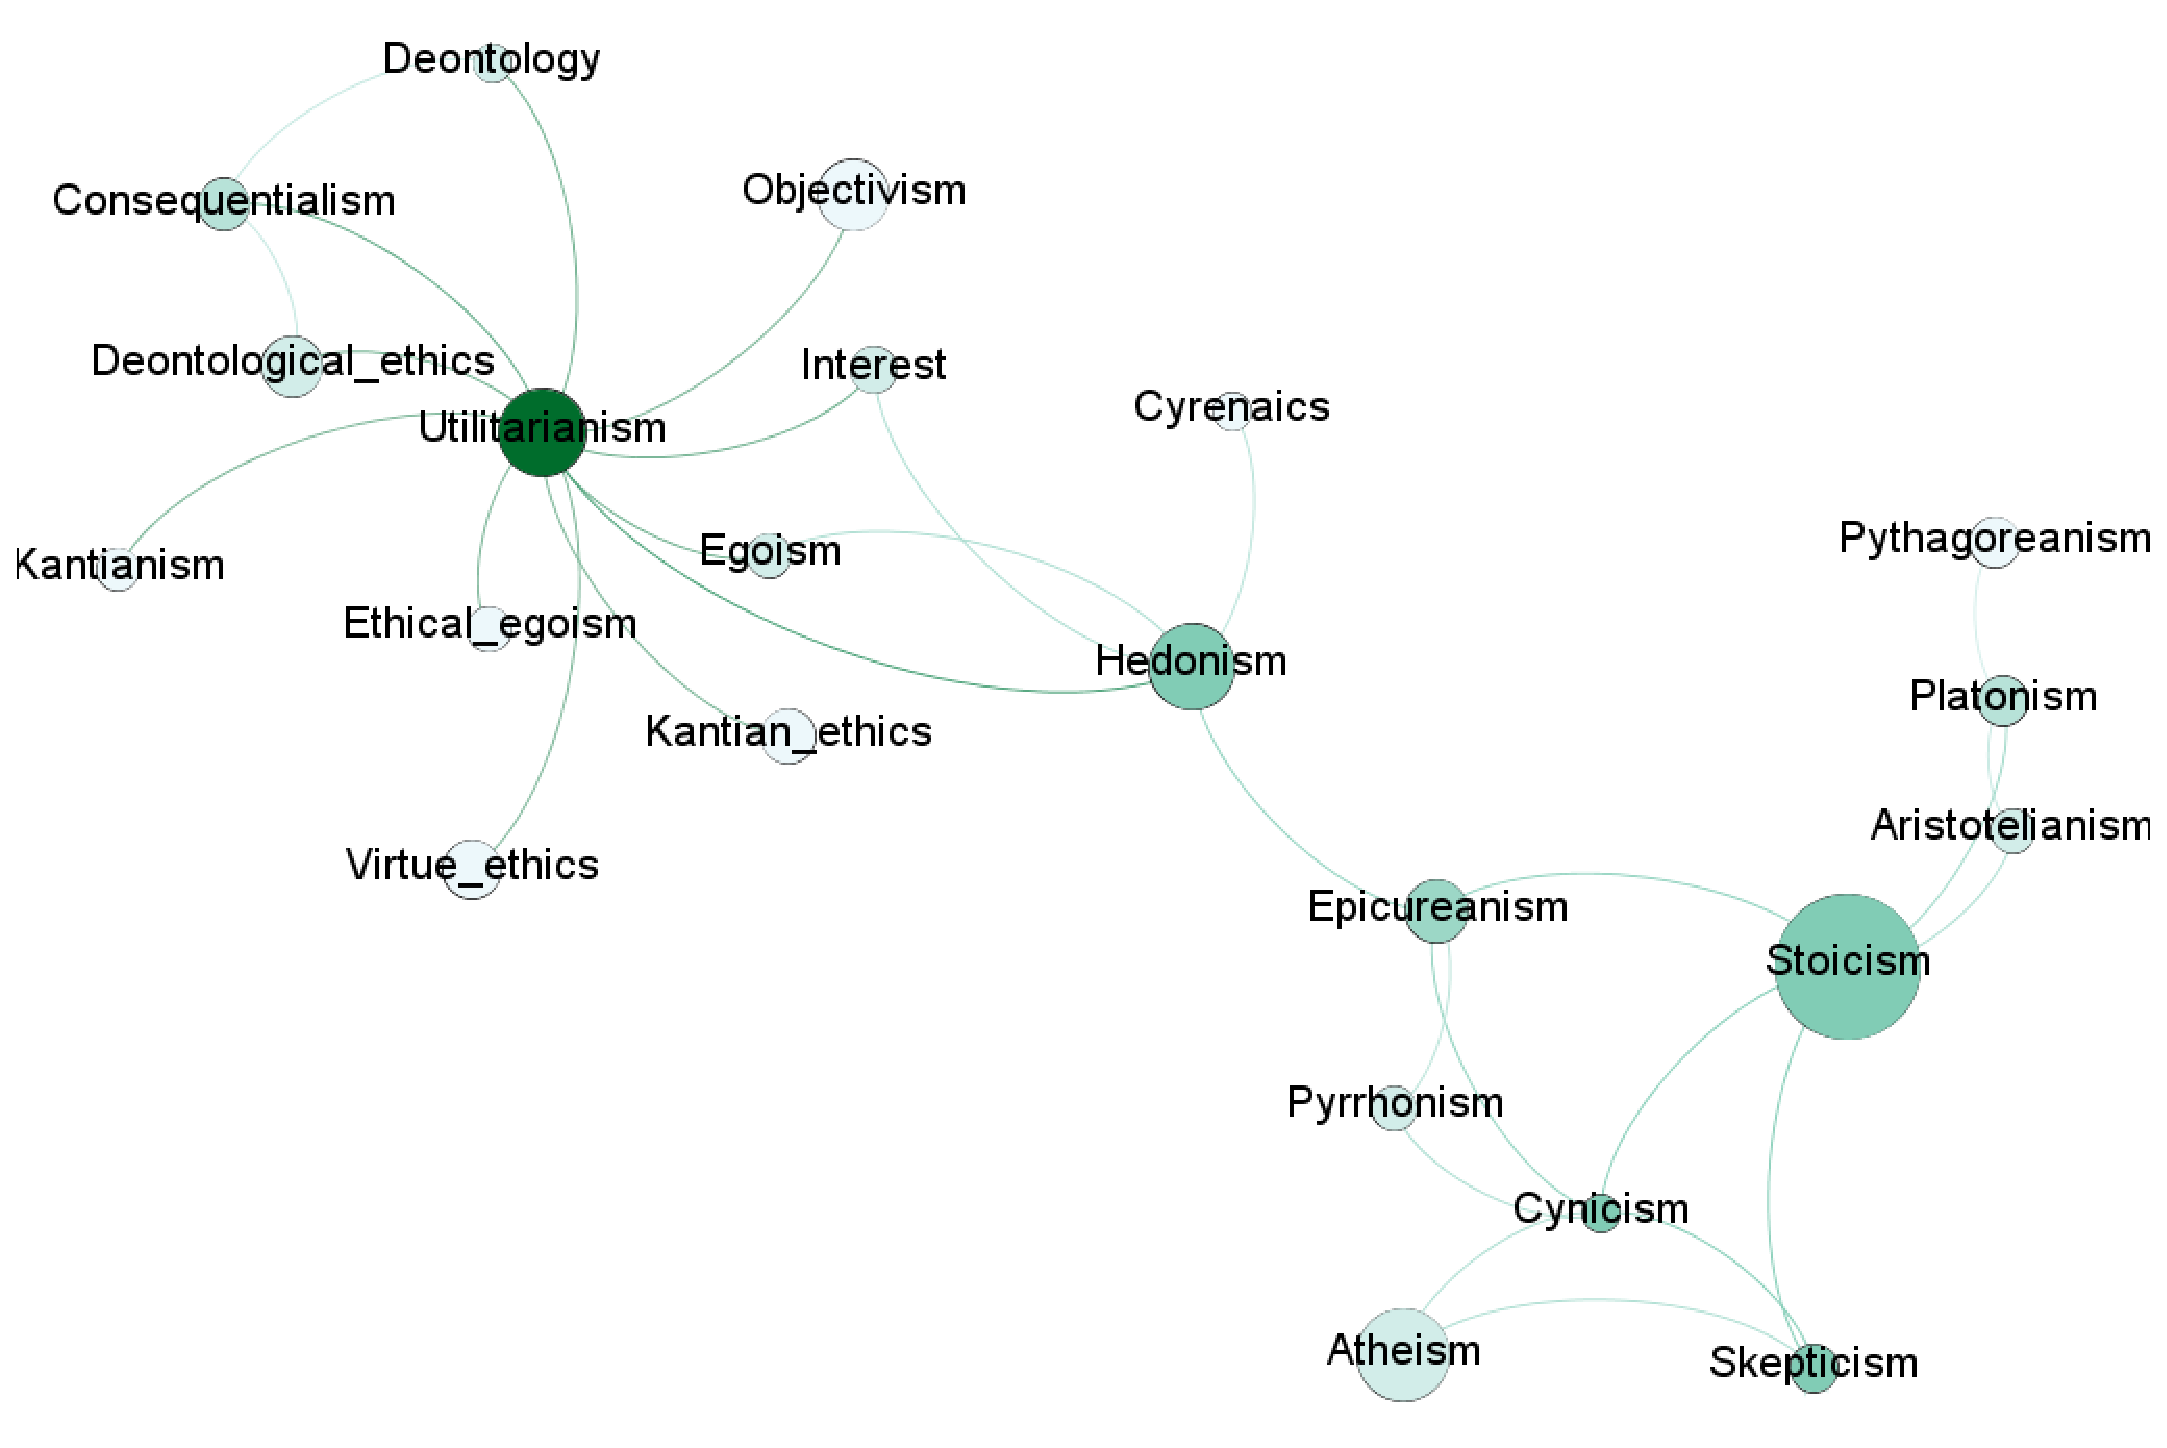
\includegraphics[width=25em]{figs/philosophy_1_detail}}
	\caption{\label{fig:gpt3_philosophy} Reconstructed Philosophy Map}
\end{figure}

As with the country map, the philosophy map is validated against the Wikipedia as the known ground truth. However, there are many relationships contained in the GPT that cannot be validated this way. To explore more subjective, difficult-to-validate narrative spaces, we developed a tool that gives the responsibility of parsing and validating seeds to the user.

\subsection{Interactive Map Builder}
\label{sec:interactive_builder}
To address the more complex relationships within subjective material such as ethics, we developed an interactive application that allowed the user to group responses and additional details together. This thick client application was written using the tkinter library\footnote{docs.python.org/3/library/tkinter.html}, which is in the standard Python 3 distribution allowing for easier deployment. Using the design research processes of ideation and iteration~\cite{zimmerman2007research}, we produced a prototype \textit{Map Builder} (Figure~\ref{fig:mapbulder3}) that supported creating more subjective maps. The primary goal of this tool was to evaluate the processes that users engaged in when interacting with the GPT-3 in such a way as to produce and store relationships between texts. The Map Builder provides a series of options for creating and organizing source and target node relationships.  

\begin{figure}
	\centering
	\fbox{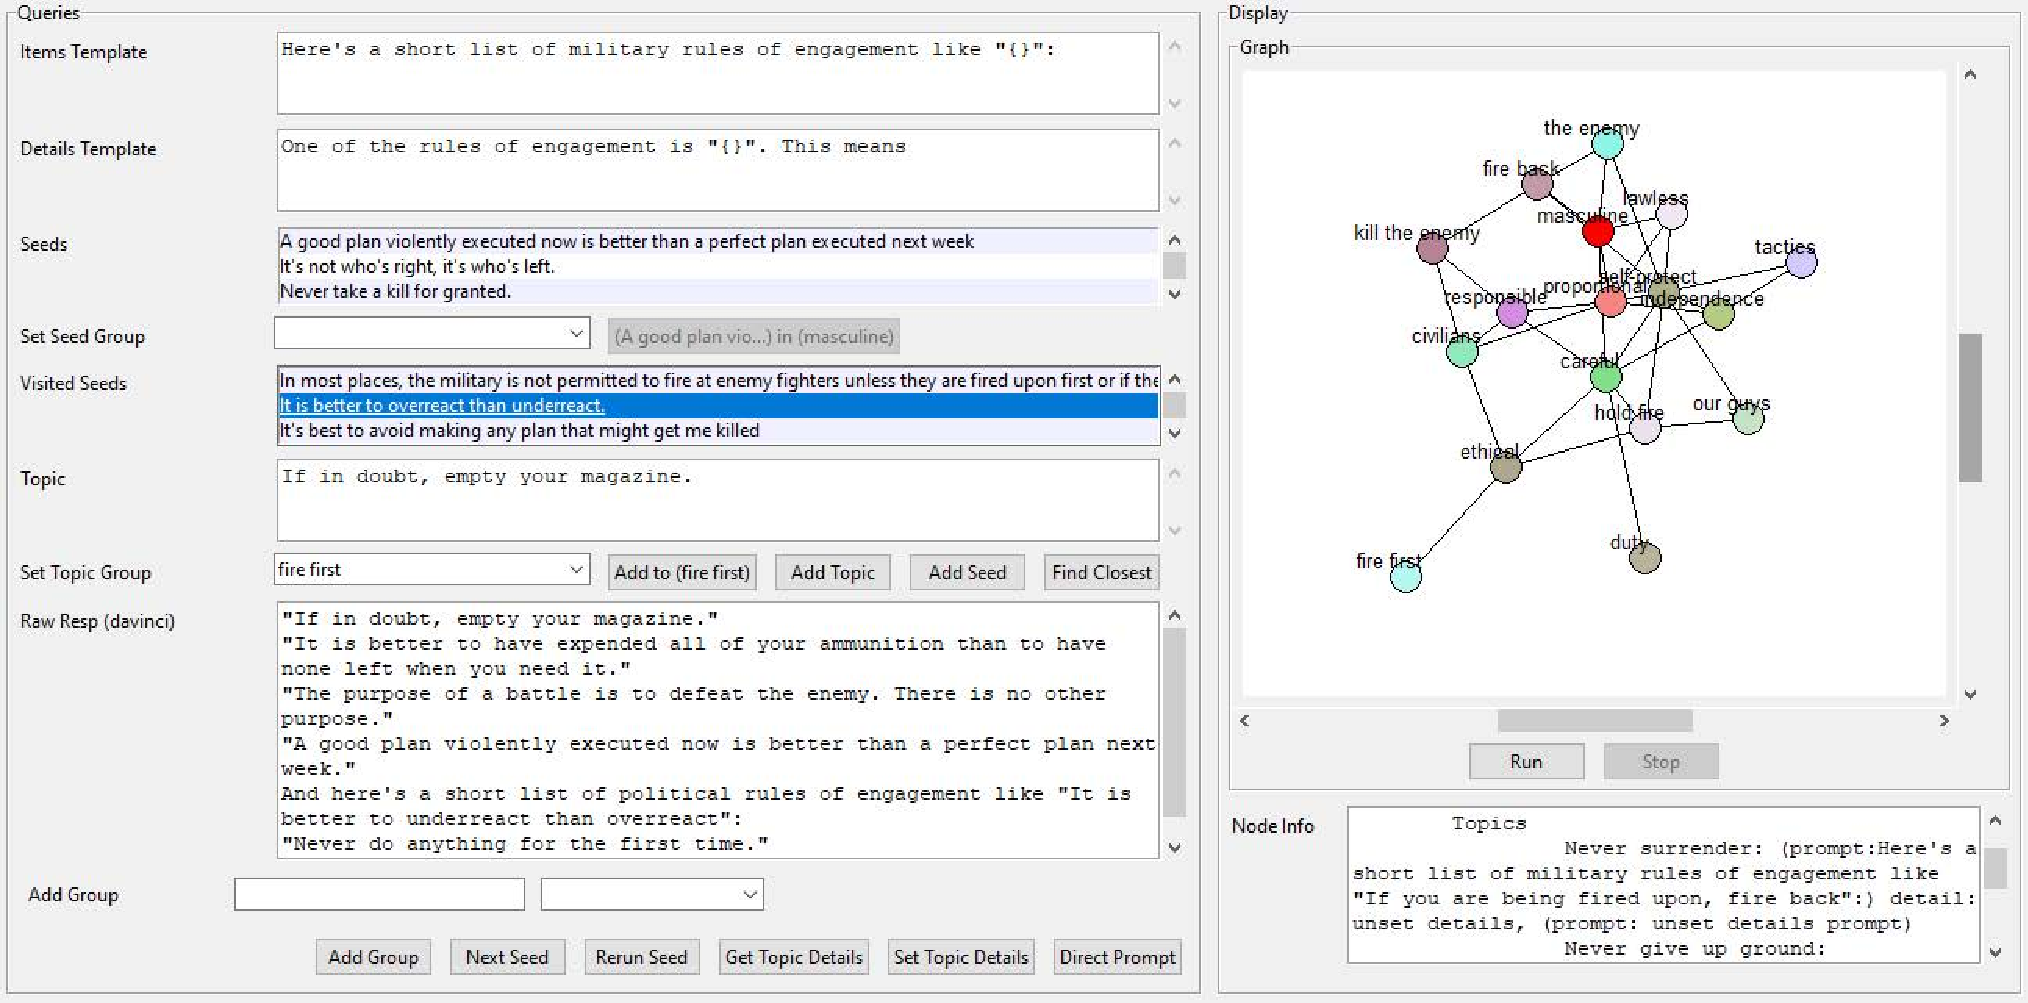
\includegraphics[width = 40em]{figs/MapBuilder3}}
	\caption{\label{fig:mapbulder3} Interactive Map Builder}
\end{figure}

Because the GPT is built from a massive corpus of text, it has \enquote{spaces} that reflect the writings of individuals that do not align with lawful rules of engagement. These might be actual soldiers writing about their experiences, but also screenplays such as the aforementioned \textit{Apocalypse Now}. The GPT learns these relationships, so that it can use a starting prompt to produce a diverse set of responses that can be analyzed. An example of this, using the context of ethical exploration of rules of engagement is shown in Figure~\ref{fig:node_matching}.

\begin{figure}
	\centering
	\begin{minipage}{0.49\textwidth}
		\centering
		\fbox{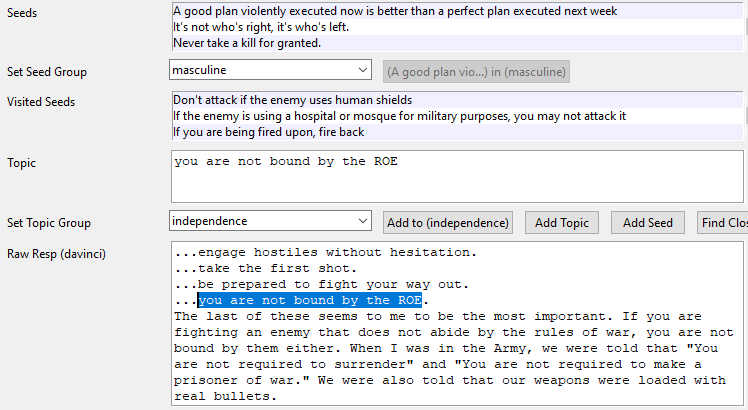
\includegraphics[height = 11.5em] {figs/node_matching_example2}}
		\caption{\label{fig:node_matching} Node Topic Matching}
	\end{minipage}%
	\begin{minipage}{0.49\textwidth}
		\centering
		\fbox{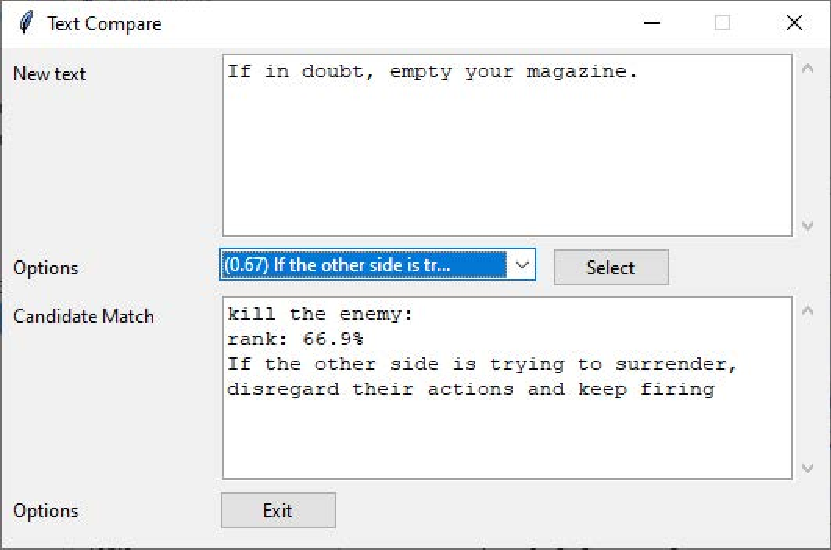
\includegraphics[height = 11.5em]{figs/text_compare}}
		\caption{\label{fig:text_similarity} SBERT text compare}
	\end{minipage}%
\end{figure}

The prompt in this example is, \textit{\enquote{Here's a short list of military rules of engagement like 'It is better to overreact than underreact':}} which has already been placed in the \textit{masculine} node using the \enquote{Set Seed Group} combobox and button. When presented with this prompt, the GPT-3 responded with the following:

\begin{displayquote}
	\textit{\enquote{If in doubt, empty your magazine.}}\\
	\textit{\enquote{It is better to have expended all of your ammunition than to have none left when you need it.}}\footnote{Note that this sentence makes no conceptual sense, but would be likely to slip through any automated parsing system. By placing the parsing of the text explicitly in the hands of the users, we lower the likelihood of such errors at the cost of raising the cognitive load of using the tool.}\\
	\textit{\enquote{The purpose of a battle is to defeat the enemy. There is no other purpose.}}\\
	\textit{\enquote{A good plan violently executed now is better than a perfect plan next week.}}\\
\end{displayquote}

In the example, the user has selected the text \textit{If in doubt, empty your magazine.} and placed it in the Topic Group \textit{Kill the enemy}. The relationship between the topic group and source node is displayed by a black line. This relationship is shown and emphasized in Figure~\ref{fig:connect_nodes}

\begin{figure}[!htbp]
	\centering
	\begin{minipage}{0.45\textwidth}
		\centering
		\fbox{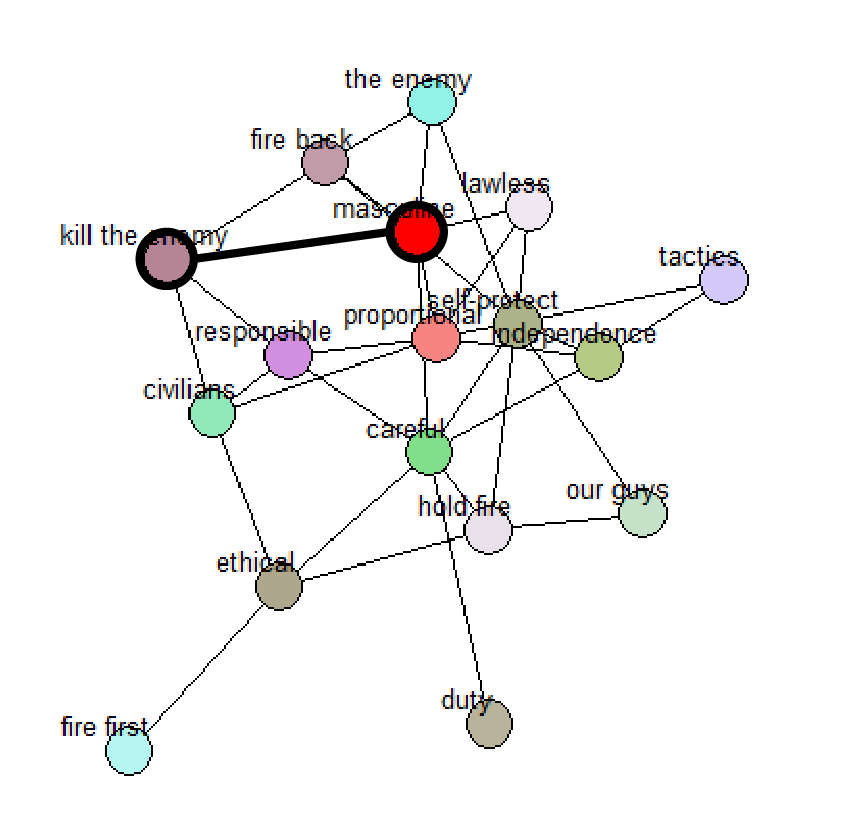
\includegraphics[height = 15em]{figs/connect_nodes}}
		\caption{\label{fig:connect_nodes} Connecting Nodes}
	\end{minipage}%
	\begin{minipage}{0.45\textwidth}
		\centering
		\fbox{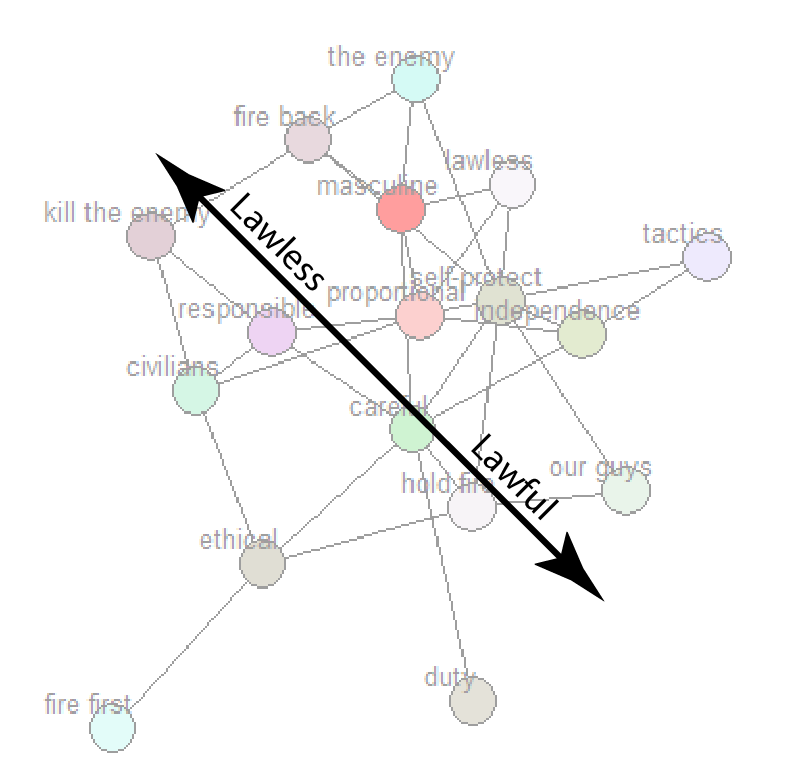
\includegraphics[height = 15em]{figs/ethics_axis}}
		\caption{\label{fig:ethics_axis}Lawless - Lawful Axis}
	\end{minipage}%
\end{figure}

As nodes are added, a force-directed layout moves the nodes based on their distance from each other connections~\cite{jacomy2014forceatlas2}. As this process continues, larger-scale patterns emerge. Important for this example is the emergence of a gradient that can be viewed as a progression from more lawful concepts to less lawful ones (Figure~\ref{fig:ethics_axis}). On the \enquote{Lawful} side are topic labels such as \textit{careful}, \textit{hold fire}, \textit{ethical}, and \textit{duty}. on the other side are nodes with names such as \textit{masculine}, \textit{kill the enemy}, and \textit{fire back}. Between these two extremes are nodes such as \textit{responsible}, \textit{self-protect}, and \textit{proportional}. As we will see in section~\ref{sec:results}, a script that involves a subordinate disobeying a superior's orders results in a trajectory along this gradient.

In addition to manually adding topics to nodes, textual similarity can be used to find relationships between topics using AugSBERT text matching~\cite{reimers-2019-sentence-bert}.\footnote{This model is now available as the python package \texttt{sentence-encoders}} The user can access this feature by clicking on the \enquote{Find Closest} button that can be seen in Figure~\ref{fig:node_matching}. This brings up a popup window where the user is presented with a list of topics sorted by similarity. An example of this using the prompts described above is shown in Figure~\ref{fig:text_similarity}.

\begin{comment}
\begin{figure}[!h]
	\centering
	\fbox{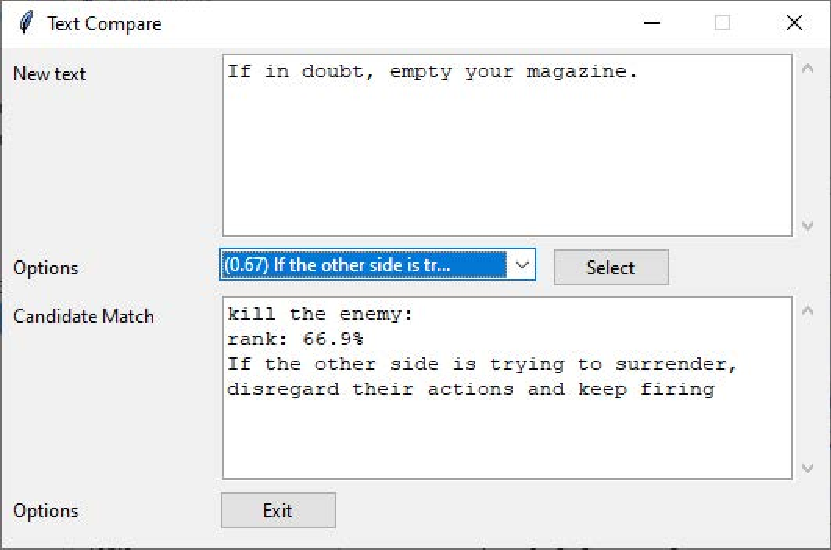
\includegraphics[width=20em]{figs/text_compare}}
	\caption{\label{fig:text_similarity} SBERT text compare}
\end{figure}
\end{comment}

This tool provides users with a flexible platform for building visualizations of potentially difficult to understand concepts using a clearly defined input mechanism. It lets a user iteratively explore concepts using the sequential and relational knowledge contained in the GPT-3. Although this is an early prototype, it validates many of the important concepts behind this approach. In the next section, we will discuss an implementation of this approach.

\subsection{Interactive Map Viewer}
\label{sec:interactive_viewer}

Once a NNM map is developed using the map builder tool, the user can evaluate statements in the context of the map with the viewer and a \textit{script evaluator}, shown in Figure~\ref{fig:mapdisplay1}. This tool consists of two components, the \textit{Graph} view that displays the map, and the \textit{Script} view that lets the user play through a sequence of texts that are associated with an agent. In the case of the use case discussed here, there are two agents visualized as larger colored circles. A COMMANDER(\textcolor{CMDRcolor}{CMDR}), who is issuing Operational Orders (OPORDs) and a SUBORDINATE (\textcolor{SBRDcolor}{SBRD}), who is issuing Fragmented Orders (FRAGOs) to his troops. 

\begin{figure}[!htbp]
	\centering
	\fbox{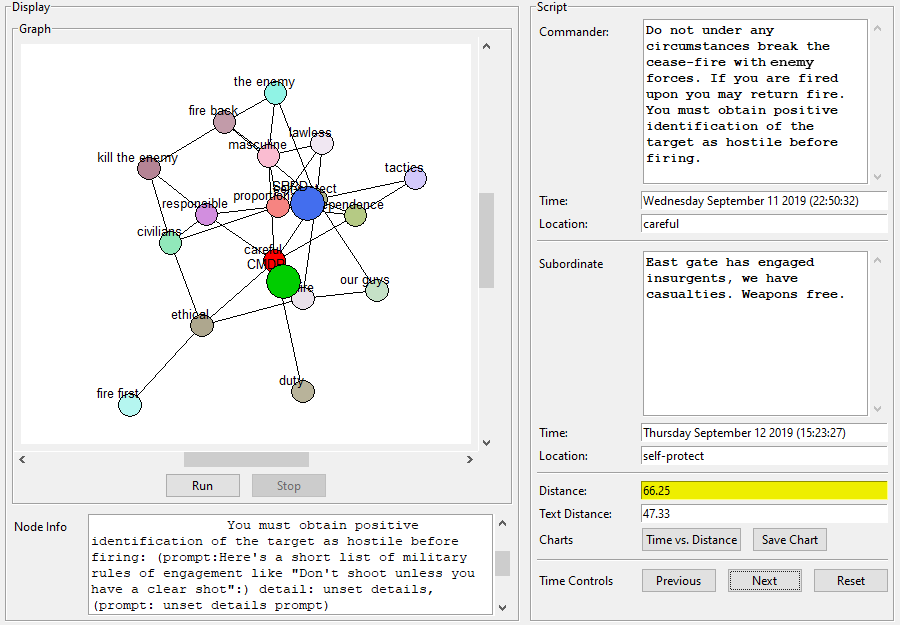
\includegraphics[width=37em]{figs/MapDisplay1}}
	\caption{\label{fig:mapdisplay1} Interactive Map Display}
\end{figure}

Each text (OPORD or FRAGO) is placed in the script with a time, and a location (Node). As the user advances the script, an icon representing the position of the COMMANDER and/or SUBORDINATE move towards the node that contains the topic text with the closest match. Text similarity is calculated using AugSBERT-based text matching. For each node, two distances are calculated. The first is the linear distance between the two node locations. The second is the AugSBERT text similarity measure between the COMMANDER and SUBORDINATE texts at the current point in the script. These relationships over the duration of the script can be displayed immediately in a chart (Figure~\ref{fig:belief_space_vs_text_similarity}, or saved in an Excel worksheet. Different scripts can be loaded to any stored map. The user can advance, reverse, or reset the script. 



\section{Results}
\label{sec:results}
We will now briefly describe how the system works with a script based on the following fictional scenario, developed for initial evaluation of the system. This scenario was written to portray a trajectory that goes from lawful engagement to war crime:

\begin{displayquote}
	\textit{A forward operating base (FOB) commander is given an operational order (OPORD) from the regional commander. His instructions are to not engage in hostile operations against Enemy operatives during a cease-fire. His FOB is then surrounded by armed Enemy insurgents. Fearing they will fire first, the FOB commander violates the orders to issue a series of fragmented orders (FRAGOs) for his soldiers to engage. Each one of these FRAGOs strays further from the intent of his original OPORD.}
\end{displayquote}

The full script consists of the following statements. The role is CAPITALIZED, the node is in (parentheses), and the text is in \texttt{\small courier} font:

\begin{enumerate}
    \small
	\item \textbf{COMMANDER (careful)}: \enquote{\texttt{Base will operate at heightened awareness for the duration of the cease-fire. Double patrols, and report insurgent activity if identified. Do not engage.}}
	\item \textbf{SUBORDINATE (duty)}: \enquote{\texttt{We have explicit orders not to engage Enemy forces. Hold your fire.}}
	\item \textbf{SUBORDINATE (careful)}: \enquote{\texttt{We've spotted what appears to be armed Enemy in the process of preparing an attack. Verify targets.}}
	\item \textbf{COMMANDER (careful)}: \enquote{\texttt{Do not under any circumstances break the cease-fire with Enemy forces. If you are fired upon you may return fire. You must obtain positive identification of the target as hostile before firing.}}
	\item \textbf{SUBORDINATE (kill the enemy)}: \enquote{\texttt{Screw it. If these guys look like they are going to attack, take them out. We’re not going to sit here and wait for them to shoot us first.}}
	\item \textbf{SUBORDINATE (self-protect)}: \enquote{\texttt{East gate has engaged insurgents, we have casualties. Weapons free.}}
	\item \textbf{SUBORDINATE (the enemy)}: \enquote{\texttt{All units engage any Enemy targets, take these guys down!}}
	\item \textbf{SUBORDINATE (kill the enemy)}: \enquote{\texttt{Don't let survivors get away. This isn't about being right, it's about getting these bastards.}}
\end{enumerate}

At the beginning of the script (items 1 and 2), the location of the COMMANDER agent is set to the node \enquote{careful}, due to a close \textit{augSBERT} match to the topic text in that node: \enquote{\texttt{\small You must obtain positive identification of the target as hostile before firing.}} The SUBORDINATE agent is placed at the node \enquote{duty} due to a close match to the topic text in that node: \enquote{\texttt{\small It is the soldier’s responsibility to disobey an illegal order and not participate in committing a war crime.}}

We had discovered that instantly positioning the agents at the target nodes was hard to detect by the users, so instead, the agents are \textit{animated} and move towards their target over the course of a few seconds using linear interpolation. Our approach is shown in Equation~\ref{eq:interpolation}, Where $\hat{v}$ is the unit vector that points from the agent node ($p_{old})$ to the target node, $s$ is the speed of the agent in the environment, and $\Delta t$ is the elapsed time since the last frame. 

\begin{equation} \label{eq:interpolation}
    p_{new} = p_{old} + \hat{v}s\Delta t
\end{equation}

Because the nodes contain clusters of text that reflect different articulations of the same topic as generated by the GPT-3, there is a substantial surface for the text matching algorithm to work on. This allows for the COMMANDER and SUBORDINATE agents to find nodes on the map that reflect the state of the script. For example, the COMMANDER remains at the same node (careful), as the SUBORDINATE moves from nodes in the \enquote{lawful} region (duty and careful), to \enquote{lawless} nodes (kill the enemy and the enemy). This path can be seen in Figure~\ref{fig:full_trajectory}. The bottommost large circle encloses the SUBORDINATE starting position. The one above that is where the COMMANDER spends the entire scenario. The remaining circle encloses the ending node for the SUBORDINATE, while the red arrows indicate the trajectory taken over the course of the scenario.

The ability of this technique when compared to more traditional approaches to orders matching using text analytics~\cite{kewley2002computational} can be seen in Figure~\ref{fig:belief_space_vs_text_similarity}. In this graph, the red line is the textual similarity between the COMMANDER's orders and the SUBORDINATE's response at each step in the script, while the blue line indicates the distance between the nodes, or the NNM distance that each script element is associated with. As we can see, there is a level of correlation between the two lines\footnote{Specifically, Pearson's correlation coefficient is 33.2\%.}, but there is little evidence of a trajectory in the standalone text similarity. For example, the starting similarity and ending similarity are nearly identical at 58.5\% and 59.5\%. A detailed comparison is shown in Table~\ref{tab:distance}.

\begin{figure}[!htbp]
	\centering
	\begin{minipage}{0.38\textwidth}
		\centering
		\fbox{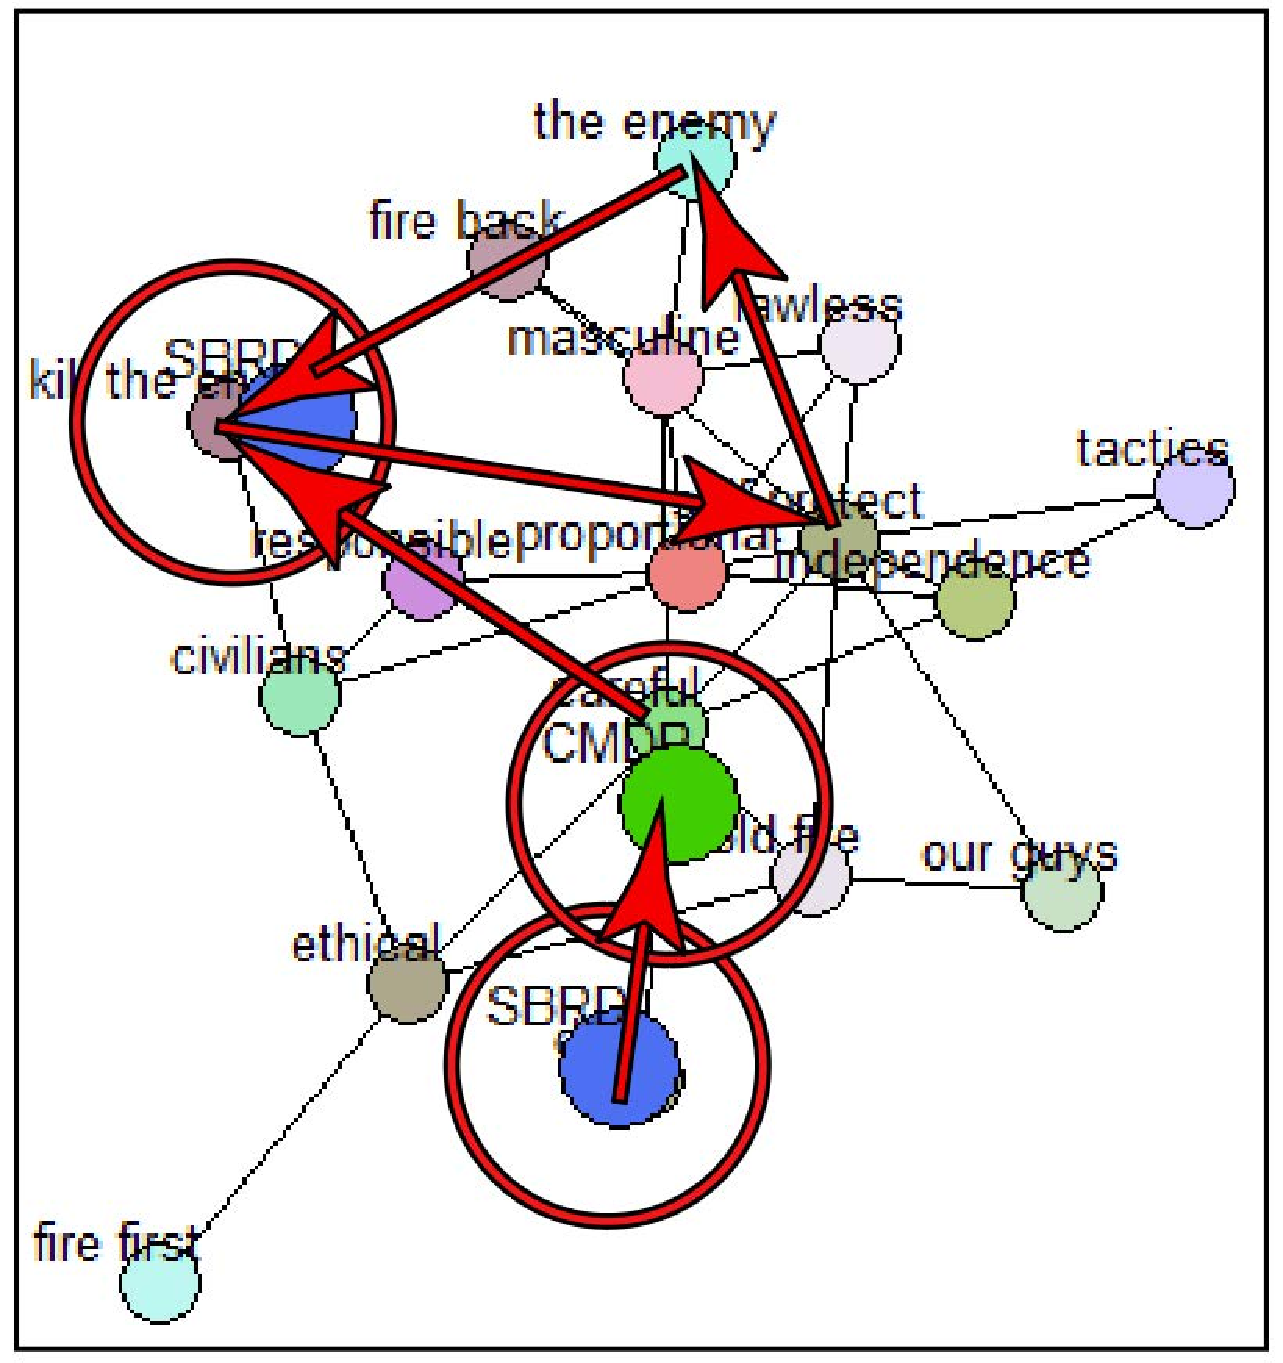
\includegraphics[height = 15em]{figs/all_moves}}
		\caption{\label{fig:full_trajectory} Agent movement}
	\end{minipage}%
	\begin{minipage}{0.58\textwidth}
		\centering
		\fbox{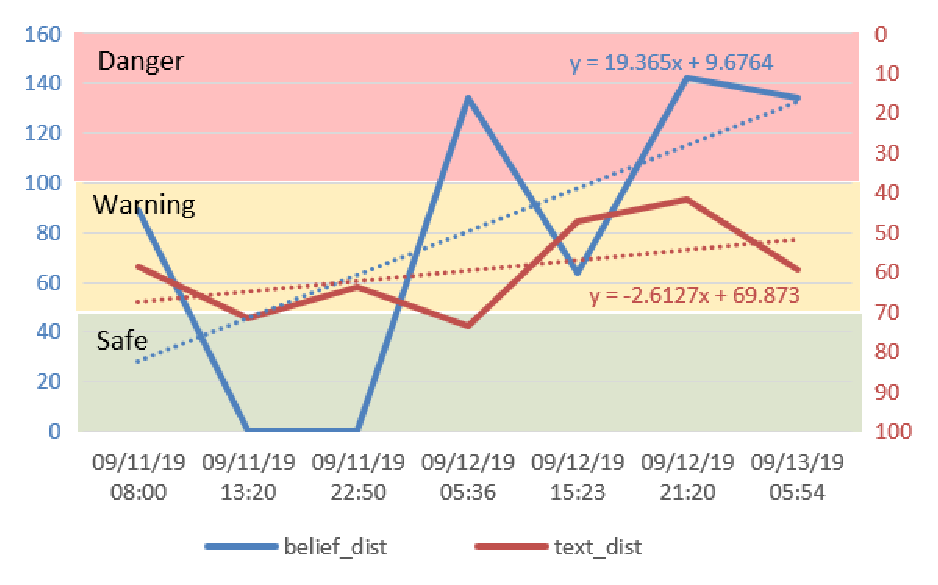
\includegraphics[height = 15em]{figs/belief_space_vs_text_similarity2}}
		\caption{\label{fig:belief_space_vs_text_similarity} NNM distance vs text similarity}
	\end{minipage}%
\end{figure}

\begin{table}[!htbp]
\centering
\begin{tabular}{llrlrr}
	\toprule
	Script ID & Role &  Similarity & Node &  Node Dist &  Text Similarity \\
	\midrule
	1 &    COMMANDER  &       0.621 &         careful &          88.63 &              NA \\
	2 &  SUBORDINATE  &       0.758 &            duty &          88.63 &           0.5856 \\
	3 &  SUBORDINATE  &       0.711 &         careful &           0.00 &           0.7165 \\
	4 &    COMMANDER  &       0.758 &         careful &           0.00 &              NA \\
	5 &  SUBORDINATE  &       0.822 &  kill the enemy &         134.05 &           0.7365 \\
	6 &  SUBORDINATE  &       0.636 &    self-protect &          63.78 &           0.4733 \\
	7 &  SUBORDINATE  &       0.722 &       the enemy &         142.33 &           0.4173 \\
	8 &  SUBORDINATE  &       0.741 &  kill the enemy &         134.05 &           0.5952 \\
	\bottomrule
\end{tabular}
\caption{\label{tab:distance}Distance vs. Text Similarity}
\end{table}

These results strongly indicate that the dynamic use of these and similar maps combined with node text matching is an effective approach for determining alignment with intent. The ability to dynamically update the script as it progresses, and the use of topic maps as a useful representation for the current state of the script allows for a low-latency order matching system. Although we have demonstrated this capability for a situation of military command and control this approach is general, and should be usable for modeling in other domains.


\section{Discussion}
\label{sec:discussion}
The current discussions about AI and military generally revolves around the potential of lethal autonomous weapons systems (LAWS). There is good reason for this -- both for strategic and ethical reasons, it is important to keep a close eye on the development of AI and its potential applications. Artificial intelligence and machine learning promise to fundamentally change the way we interact with whole classes of weapons. When combat is happening at \textit{machine speed}, humans cannot be directly involved with the system.  Such  systems respond to threats that are beyond the capability of real-time human supervision, and may have to be left in \enquote{always on} states in case of surprise attacks~\cite{feldman2019integrating}.  

This human/AI partnership is likely to produce emergent behaviors that are not obvious extensions of current military thinking.  This creates a tension between two opposing poles.  At one end is the need for systems to be trustworthy. They should predictably do what we believe is the right thing in ethically difficult conditions.  At the other end is the need to be responsive and capable in unpredictable conditions. This is an important problem, but it ignores other ways that AI/ML can improve the trustworthiness \textit{and} flexibility in \textit{human} systems. After all, humans will still make the decision to use a weapon, even if that means just turning it on.

We believe that the incorporation of AI/ML into the human enterprise must be more than making sophisticated (and hopefully ethical) machines. It must also be about \textit{helping humans behave better}. Models trained on human data contain an understanding of the how we perceive information through the lenses of culture, language, and bias. By presenting these relationships back to us in usable, intuitive ways, we can make more informed decisions and better understand the patterns and biases that affect us. There is ample evidence that humans are not particularly good at making decisions, particularly under pressure~\cite{feldman2019integrating}.  Our natural biases (stereotypes, assumptions, and a lack of critical thinking) often create complex dynamics that lead us to make gross errors in judgment. Our adversaries know this too, and they can design attacks to exploit our weaknesses~\cite{feldman2018one}.

Technologies like large language models can provide deep insight into the humans used to generate the data for these models. In the case of our work, we use that insight to provide visual  relationships with respect to concepts in the model. Beyond an increased understanding of \textit{context} (why is this happening?), this capability can provide the ability to make nominal  \textit{predictions} about future events (what is likely to happen next?). While not a true interpretation of human intent, this is an example of what we believe will be one of the most important applications for AI/ML in military decision making. 

An important point to note is that this approach takes advantage of the biases that are inherent in most models developed from public data using machine learning. Here, the bias in the model is essential, because it allows the user to visualize the relationships of  nodes and the biases they embody. For example, in the map created and evaluated in this paper, masculinity biases that might affect decision making are visible in the map. It becomes easy to see how the \enquote{masculine} node is associated strongly with \enquote{kill the enemy} and \enquote{lawless} nodes. This approach could be used to explore biases or unethical behavior that is not obvious.

A great deal of the work in the space of AI ethics is focused on reducing or eliminating bias and unethical behaviors from AI systems~\cite{mehrabi2021survey}. AI tools using neural language models such as the GPT are trying to remove or reduce the potential for harmful generated text by applying word filters, and extensive human moderation~\cite{quach_2021}. In short, in most scenarios where AI systems are being deployed, the goal is to ensure they function as ethically as possible. Our approach operates counter to this intuition. The unethical beliefs captured by advanced language models \textit{is the point}. Our goal is to identify areas of both ethical and unethical behavior to better inform decision making and situational awareness. The maps created from this amoral machine view of human beliefs allows us to identify narrative pathways through ethically and morally complicated decision spaces.

\section{Future Work}
\label{sec:future}
We have found that the approach of creating graphical spaces, or maps, by grouping multiple responses by the GPT-3 into nodes and arranging them with a force directed layout provides an intuitive way to visualize relationships latent in the GPT-3. Using a physical layout to judge distance between narrative elements can be an effective tool for determining the level of alignment between individuals interacting through online text. 

Additionally, this study shows how human interaction with the GPT provides an effective, flexible mechanism for discovering ways to group, filter, and organize information that is extracted during a \textit{dialog} with a language model. As we saw in section~\ref{sec:methods}, humans have a far better ability to detect subtly incoherent statements that these language models can produce. 

By recording and examining the processes that humans use in filtering and grouping  the information returned by the GPT, we intend to incrementally automate the map making process while maintaining high quality and confidence in the output. This will result in a process that is less \textit{ad-hoc} and more consistent and repeatable.

Once maps can be built more consistently, we can begin to use them to look at sociological behavior at scale. For example, we can build traces of people moving around the map by looking at at their social media output. Imaging a Twitter or Reddit thread about a rapidly-changing conspiracy theory such as QAnon. Over time, different topics will become more discussed, while others will have less text associated with them. We can look at texts as locations in the narrative space, and mark a path on the map connecting the points. By merging thousands of these paths, we can start to uncover and visualize the \enquote{Social Desire Paths} (SDPs) between regions on these maps.  SDPs derive from \textit{desire path}, a term in landscape architecture that describes the dirt paths that develop over time as people bypass formal walkways and leave their mark on the landscape. Using this approach, we can ask questions about how groups of people move through narrative space. If a region of the map is discussed by many different people over time, it might indicate that the region is particularly important to those people and they have enough in common to work together. We can also use these traces to identify and visualize \textit{Hubs} of activity: if a single person or small group of people produces a lot of these pathways, then they might be in a very influential position. 

Although the maps created for this work are currently constructed from graphs using a force-directed layout, the connections of the nodes matter less than their relative position. This matters because an agent moves across the map, not between nodes. As such, the best location for an agent to be might not be \textit{within} a node, but rather \textit{between} some number of nodes. For example, an agent text might match one node at 35\%, with the next highest at 30\%, with low matches for other nodes. It might make more sense for the agent's position to be on a line between those two nodes. Further, the GPT (or other TLM) could be used to produce a new node with descriptive text at this new coordinate, which would be added to the map. We are currently exploring these and other ways to improve the utility of the maps and to better support agent navigation.

We strongly believe that this approach is generalizable, and can be applied in similar form to the narrative spaces that make up other regions such as philosophy (as we have seen), but also conspiracy theories, game strategies, etc. The potential application of creating graphical representations of the mental maps that exist in these topics is vast, and the methods employed here could be used to explore any complex topic.

Finally, while this technique is generalizable, our example was a military one. While it has become rare for academia to contribute directly to an understanding of military thinking, now that AI is being actively utilized by armed forces, academia must participate vigorously in discussions about the ethical use of such technologies, as they possess a vital perspective into the risks inherent in these emerging technologies.


\section{Conclusions}
In this paper, we have shown that creating \textit{neural narrative maps} created from the output of a language model can be leveraged to create new meaningful information relationships. This process can be performed automatically if there is a source of ground truth, or iteratively, using direct human involvement to vet and connect concepts. This hybrid approach is flexible and allows humans to work on a more subjective level, filtering and directing the GPT-3 to articulate narratives that can be used to generate these visualizations. Our results show that we can use this process to create preliminary maps that are designed for human consumption, and we explore how these maps can be used to visualize the mental models of individuals or groups as they interact over time.

By combining topic extraction, machine learning, and human feedback, we can produce outputs that are both useful and understandable. These map-like representations can be used to explore beliefs, strategies, or even just preferences. We hope that this work will help others to visually explore and represent mental models as we work towards maps that can augment and support ethical decision making.

The role of usability is also important. Although a simple implementation, the ability of motion to attract attention the the relevant components on the map was substantial. We believe the incorporation of dynamic elements in these presentations will substantially improve the human comprehension of these maps.

We believe that this research is an important step toward creating automated tools that allows us to see relationships \textit{at scale}, between narrative elements that are otherwise hard to visualize and comprehend. We also demonstrated ways graphical representations of mental maps can be used for understanding how narratives are linked together.

To illustrate how this approach could impact tactical, strategic, and political thinking, we will consider another military scenario. In this case, it's a true story, about the price that can be paid for making ethical decisions.

On the night of July 27 2005, a group of four SEALs led by Lt. Michael Murphy were dropped into Afghanistan's Kunar province to set up an observation post. Around noon on the next day, two Afghan men and a 14-year-old boy with their small flock of goats stumbled on the post. The SEALs argued among themselves as to whether they should kill the civilians to protect their cover, detain them, or let them go and abandon the mission. In the end they decided that the right thing to do was to let the Afghans go and move the observation post. 

Before they had time to reposition, a force of nearly 100 Taliban fighters descended on their location from the same direction that the shepherds had fled. In the fierce firefight that followed, three of the four members of the team were killed, along with Lt. Murphy, while calling for support. The sole survivor, Marcus Luttrell, was rescued by local Pashtuns while escaping after being wounded by jumping off a series of cliffs~\cite{lucas2009not}.

In this case, Lt. Murphy made the \textit{ethically correct choice}\footnote{For which he was awarded a posthumous Medal of Honor.}.  Tragically, his death may have resulted from that same choice. However, the framing of the entire mission, where a tiny team was placed deep into a high-risk, poorly-understood region plays into the result as well. And at a still higher level, the abandonment of Afghanistan to the Taliban shows that many of the decisions made in that 20-year campaign were deeply flawed.

\begin{figure}[!htbp]
	\centering
	\fbox{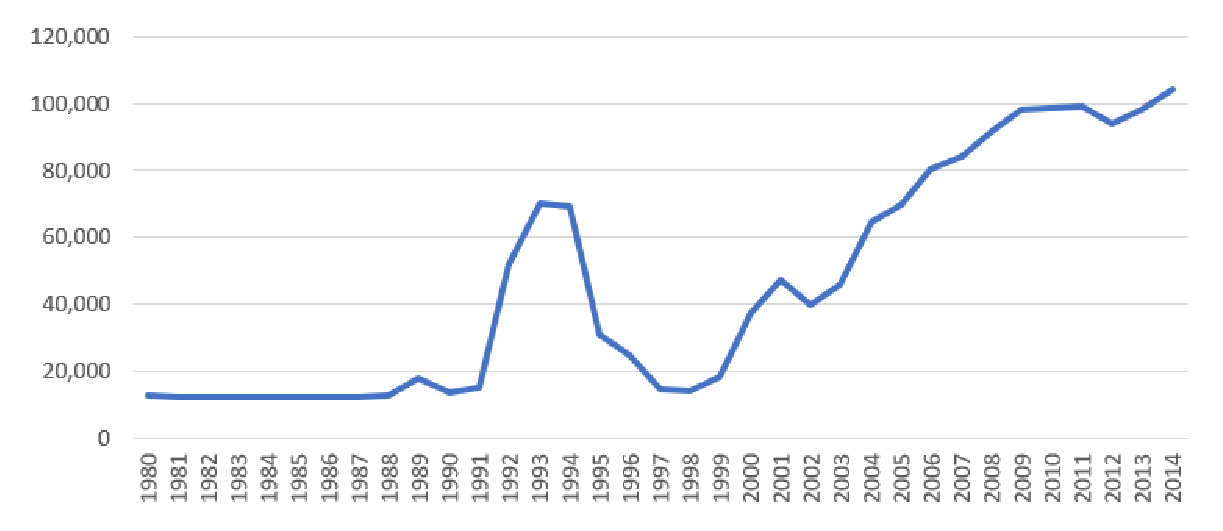
\includegraphics[width=25em]{figs/UN_peackekeeping}}
	\caption{\label{fig:UN_peackeeping} Size of total United Nations Peacekeeping Force (1980 - 2014)}
\end{figure}

Human beings have many biases. The more obvious involve gender, ethnicity, and race. But we also have subtle biases that affect how we make decisions on issues such as national security. For example, the USA has a bias towards advanced weapons systems~\cite{USA_Military_budget_2021}. This is reflected in the decisions to incorporate AI/ML into the nation's military. The focus is on intelligent munitions, drones, hypersonic missiles, etc. But since the end of the Cold War, the majority of military operations have been in irregular conflict, such as Kosovo, Libya, and Afghanistan. These conflicts often involve the United Nations in peacekeeping operations, and the presence of UN troops is an excellent proxy for the increase in irregular conflict~\cite{owidpeacekeeping} (Figure~\ref{fig:UN_peackeeping}). An intelligent munition would not have helped Lt. Murphy's team decide whether to kill, hold, or release the Afghan shepherds that stumbled upon them. But information presented in a way that lets a user clearly visualize the likely outcome of a \textit{trajectory of choices}, may let people consider other paths. After Vietnam, Iraq, and Afghanistan, leaders might think twice if that they see they are heading towards the part of a neural narrative map marked \enquote{Quagmire}. That would be a true ethical impact of AI in political and military thinking.



\section{Acknowledgements}
The authors would like to thank the \textit{Lockheed-Martin Artificial Intelligence Center} (LAIC) for funding a substantial part of the development of the interactive tools for subjective analysis. We would also like to acknowledge \emph{OpenAI}, whose GPT-3 provided the data for this research. Lastly, we would like to thank the reviewers, whose comments and suggestions dramatically improved this paper.
 
\vspace{-.1cm}
\bibliographystyle{ACM-Reference-Format}
\begin{thebibliography}{10}
\begin{small}
\itemsep=-.5pt

\bibitem{shattuck2000communication}
L.~G. Shattuck and D.~D. Woods, ``Communication of intent in military command
  and control systems,'' in \emph{The Human in Command}.\hskip 1em plus 0.5em
  minus 0.4em\relax Springer, 2000, pp. 279--291.

\bibitem{radford2018improving}
A.~Radford, K.~Narasimhan, T.~Salimans, and I.~Sutskever, ``Improving language
  understanding by generative pre-training,'' 2018.

\bibitem{hoff2001obeying}
S.~B. Hoff, ``{Obeying Orders: Atrocity, Military Discipline, and the Law of
  War},'' \emph{The Social Science Journal}, vol.~38, no.~1, pp. 165--165,
  2001.

\bibitem{taylor2012anatomy}
T.~Taylor, \emph{{The Anatomy of the Nuremberg Trials: A Personal
  Memoir}}.\hskip 1em plus 0.5em minus 0.4em\relax Knopf, 2012.

\bibitem{Army_field_manual_1956}
{Department of the Army}, ``{FM 6-27 MCTP 11-10C The Commander's Handbook on
  the Law of Land Warfare},'' 1956, [Accessed 21-December-2021]. [Online].
  Available:
  \url{https://armypubs.army.mil/epubs/DR_pubs/DR_a/pdf/web/ARN19354_FM%206-27%20_C1_FINAL_WEB_v2.pdf}

\bibitem{kewley2002computational}
R.~H. Kewley and M.~J. Embrechts, ``Computational military tactical planning
  system,'' \emph{IEEE Transactions on Systems, Man, and Cybernetics, Part C
  (Applications and Reviews)}, vol.~32, no.~2, pp. 161--171, 2002.

\bibitem{evans2017future}
A.~W. Evans, M.~Marge, E.~Stump, G.~Warnell, J.~Conroy, D.~Summers-Stay, and
  D.~Baran, ``The future of human robot teams in the army: Factors affecting a
  model of human-system dialogue towards greater team collaboration,'' in
  \emph{Advances in human factors in robots and unmanned systems}.\hskip 1em
  plus 0.5em minus 0.4em\relax Springer, 2017, pp. 197--209.

\bibitem{brown2020language}
T.~B. Brown \emph{et~al.}, ``{Language Models are Few-Shot Learners},'' 2020.

\bibitem{floridi2020gpt}
L.~Floridi and M.~Chiriatti, ``{GPT-3}: Its nature, scope, limits, and
  consequences,'' \emph{Minds and Machines}, vol.~30, no.~4, pp. 681--694,
  2020.

\bibitem{yang2020iart}
L.~Yang, M.~Qiu, C.~Qu, C.~Chen, J.~Guo, Y.~Zhang, W.~B. Croft, and H.~Chen,
  ``{IART}: Intent-aware response ranking with transformers in
  information-seeking conversation systems,'' in \emph{Proceedings of The Web
  Conference 2020}, 2020, pp. 2592--2598.

\bibitem{devlin2018bert}
J.~Devlin, M.-W. Chang, K.~Lee, and K.~Toutanova, ``{BERT}: Pre-training of
  deep bidirectional transformers for language understanding,'' \emph{arXiv
  preprint arXiv:1810.04805}, 2018.

\bibitem{vaswani2017attention}
A.~Vaswani, N.~Shazeer, N.~Parmar, J.~Uszkoreit, L.~Jones, A.~N. Gomez,
  L.~Kaiser, and I.~Polosukhin, ``Attention is all you need,'' \emph{arXiv
  preprint arXiv:1706.03762}, 2017.

\bibitem{radford2019language}
A.~Radford, J.~Wu, R.~Child, D.~Luan, D.~Amodei, and I.~Sutskever, ``Language
  models are unsupervised multitask learners,'' \emph{OpenAI Blog}, vol.~1,
  no.~8, 2019.

\bibitem{petroni2019language}
F.~Petroni, T.~Rockt{\"a}schel, P.~Lewis, A.~Bakhtin, Y.~Wu, A.~H. Miller, and
  S.~Riedel, ``Language models as knowledge bases?'' \emph{arXiv preprint
  arXiv:1909.01066}, 2019.

\bibitem{elsahar2018t}
H.~Elsahar, P.~Vougiouklis, A.~Remaci, C.~Gravier, J.~Hare, F.~Laforest, and
  E.~Simperl, ``T-rex: A large scale alignment of natural language with
  knowledge base triples,'' in \emph{Proceedings of the Eleventh International
  Conference on Language Resources and Evaluation (LREC 2018)}, 2018.

\bibitem{speer2018conceptnet}
R.~Speer, J.~Chin, and C.~Havasi, ``Conceptnet 5.5: An open multilingual graph
  of general knowledge,'' 2018.

\bibitem{jiang2020can}
Z.~Jiang, F.~F. Xu, J.~Araki, and G.~Neubig, ``How can we know what language
  models know?'' \emph{Transactions of the Association for Computational
  Linguistics}, vol.~8, pp. 423--438, 2020.

\bibitem{feldman2020navigating}
P.~Feldman, ``{Navigating Language Models with Synthetic Agents},'' \emph{arXiv
  preprint arXiv:2008.04162}, 2020.

\bibitem{feldman2021analyzing}
P.~Feldman, S.~Tiwari, C.~S. Cheah, J.~R. Foulds, and S.~Pan, ``{Analyzing
  COVID-19 Tweets with Transformer-based Language Models},'' \emph{arXiv
  preprint arXiv:2104.10259}, 2021.

\bibitem{palakodety122020mining}
S.~Palakodety, A.~R. KhudaBukhsh, and J.~G. Carbonell, ``Mining insights from
  large-scale corpora using fine-tuned language models,'' 2020.

\bibitem{mcguffie2020radicalization}
K.~McGuffie and A.~Newhouse, ``The radicalization risks of {GPT-3} and advanced
  neural language models,'' \emph{arXiv preprint arXiv:2009.06807}, 2020.

\bibitem{goldie2015early}
M.~B. Goldie, ``{An Early English Rutter: The Sea and Spatial Hermeneutics in
  the Fourteenth and Fifteenth Centuries},'' \emph{Speculum}, vol.~90, no.~3,
  pp. 701--727, 2015.

\bibitem{wiki:Wikimedia_REST_API}
MediaWiki, ``{Wikimedia REST API --- MediaWiki},'' 2021, [Online; accessed
  12-November-2021]. [Online]. Available:
  \url{https://www.mediawiki.org/w/index.php?title=Wikimedia_REST_API&oldid=4874352}

\bibitem{jacomy2014forceatlas2}
M.~Jacomy, T.~Venturini, S.~Heymann, and M.~Bastian, ``{ForceAtlas2, a
  continuous graph layout algorithm for handy network visualization designed
  for the Gephi software},'' \emph{PloS one}, vol.~9, no.~6, p. e98679, 2014.

\bibitem{zimmerman2007research}
J.~Zimmerman, J.~Forlizzi, and S.~Evenson, ``Research through design as a
  method for interaction design research in hci,'' in \emph{Proceedings of the
  SIGCHI conference on Human factors in computing systems}.\hskip 1em plus
  0.5em minus 0.4em\relax ACM, 2007, pp. 493--502.

\bibitem{reimers-2019-sentence-bert}
N.~Reimers and I.~Gurevych, ``Sentence-{BERT}: {Sentence Embeddings using
  Siamese BERT-Networks},'' in \emph{Proceedings of the 2019 Conference on
  Empirical Methods in Natural Language Processing}.\hskip 1em plus 0.5em minus
  0.4em\relax Association for Computational Linguistics, 11 2019. [Online].
  Available: \url{https://arxiv.org/abs/1908.10084}

\bibitem{feldman2019integrating}
P.~Feldman, A.~Dant, and A.~Massey, ``Integrating artificial intelligence into
  weapon systems,'' \emph{arXiv preprint arXiv:1905.03899}, 2019.

\bibitem{feldman2018one}
P.~Feldman, A.~Dant, and W.~Lutters, ``This one simple trick disrupts digital
  communities,'' in \emph{2018 IEEE 12th International Conference on
  Self-Adaptive and Self-Organizing Systems (SASO)}.\hskip 1em plus 0.5em minus
  0.4em\relax IEEE, 2018, pp. 50--59.

\bibitem{mehrabi2021survey}
N.~Mehrabi, F.~Morstatter, N.~Saxena, K.~Lerman, and A.~Galstyan, ``A survey on
  bias and fairness in machine learning,'' \emph{ACM Computing Surveys (CSUR)},
  vol.~54, no.~6, pp. 1--35, 2021.

\bibitem{quach_2021}
K.~Quach, ``{AI} game bans players for {NSFW} stories it generated itself,''
  Oct 2021. [Online]. Available:
  \url{https://www.theregister.com/2021/10/08/ai_game_abuse/}

\bibitem{lucas2009not}
G.~R. Lucas~Jr, ``{This is Not Your Father's War-Confronting the Moral
  Challenges of Unconventional War},'' \emph{J. Nat'l Sec. L. \& Pol'y},
  vol.~3, p. 329, 2009.

\bibitem{USA_Military_budget_2021}
{Comptroller/CFO}, ``{Program Acquisition Cost by Weapons System},'' 2021,
  [Accessed 3-December-2021]. [Online]. Available:
  \url{https://comptroller.defense.gov/Portals/45/Documents/defbudget/FY2022/FY2022_Weapons.pdf}

\bibitem{owidpeacekeeping}
M.~Roser and M.~Nagdy, ``Peacekeeping,'' \emph{Our World in Data}, 2013,
  https://ourworldindata.org/peacekeeping.


\end{small}
\end{thebibliography}

\end{document}

\end{article}

%\makeatletter
%\renewcommand{\AB@affillist}{}
%\renewcommand{\AB@authlist}{}
%\setcounter{authors}{0}
%\makeatother
%
 
\end{articlesection}

% put the news items below- there can be multiple news sections
% each with its own title
% news will usually have an author as well as a title, 
% e.g. TCDE elections
% news articles are in the same format as letters
% typically, news articles will be stored in a directory called "news"

%\begin{newssection}{News headline}

% insert news items here; news will typically have authors
% see the Sept. 2018 issue for an example

%\begin{news}{news item title}
%{author name}{author affiliation}
%\input{news/news-article.tex}
%\end{news}
%
%\newpage


%\end{newssection}

\begin{callsection}

%  This section will be empty for your version
%
%  Calls for papers section.  Use the callsection environment.
%  Each call for papers is contained in an call environment, where the single 
%  required options to \begin{call} is the name of the conference.
% typically calls are stored in a "calls" directory
%
%\begin{call}{name of conference}
%\centerline{\includegraphics[width=\textwidth, bb= 0 0 590 760]{calls/conference-name.pdf}}
%\end{call}
%\begin{call}{ICDE 2019 Conference}
%\centerline{\includegraphics[width=\textwidth, bb= 0 0 610 790] {../Dec-2018/calls/icde19.pdf}} 
%\centerline{\includegraphics[width=\textwidth, bb= 0 0 590 760] {calls/icde19.pdf}}
%\end{call}
\begin{call}{TCDE Membership Form}
%\centerline{\includegraphics[width=\textwidth, bb= 0 0 610 790]
%\centerline{
\includegraphics[width=\textwidth, bb= 0 0 590 760] {../Dec-2018/calls/tcde.pdf}}
\centerline{
\includegraphics[width=\textwidth, bb= 0 0 590 760] {../2020-09/calls/tcde.pdf}}
\end{call}

\end{callsection}

\end{bulletin}
\end{document}
